\documentclass[twoside]{book}

% Packages required by doxygen
\usepackage{fixltx2e}
\usepackage{calc}
\usepackage{doxygen}
\usepackage[export]{adjustbox} % also loads graphicx
\usepackage{graphicx}
\usepackage[utf8]{inputenc}
\usepackage{makeidx}
\usepackage{multicol}
\usepackage{multirow}
\PassOptionsToPackage{warn}{textcomp}
\usepackage{textcomp}
\usepackage[nointegrals]{wasysym}
\usepackage[table]{xcolor}

% Font selection
\usepackage[T1]{fontenc}
\usepackage[scaled=.90]{helvet}
\usepackage{courier}
\usepackage{amssymb}
\usepackage{sectsty}
\renewcommand{\familydefault}{\sfdefault}
\allsectionsfont{%
  \fontseries{bc}\selectfont%
  \color{darkgray}%
}
\renewcommand{\DoxyLabelFont}{%
  \fontseries{bc}\selectfont%
  \color{darkgray}%
}
\newcommand{\+}{\discretionary{\mbox{\scriptsize$\hookleftarrow$}}{}{}}

% Page & text layout
\usepackage{geometry}
\geometry{%
  a4paper,%
  top=2.5cm,%
  bottom=2.5cm,%
  left=2.5cm,%
  right=2.5cm%
}
\tolerance=750
\hfuzz=15pt
\hbadness=750
\setlength{\emergencystretch}{15pt}
\setlength{\parindent}{0cm}
\setlength{\parskip}{3ex plus 2ex minus 2ex}
\makeatletter
\renewcommand{\paragraph}{%
  \@startsection{paragraph}{4}{0ex}{-1.0ex}{1.0ex}{%
    \normalfont\normalsize\bfseries\SS@parafont%
  }%
}
\renewcommand{\subparagraph}{%
  \@startsection{subparagraph}{5}{0ex}{-1.0ex}{1.0ex}{%
    \normalfont\normalsize\bfseries\SS@subparafont%
  }%
}
\makeatother

% Headers & footers
\usepackage{fancyhdr}
\pagestyle{fancyplain}
\fancyhead[LE]{\fancyplain{}{\bfseries\thepage}}
\fancyhead[CE]{\fancyplain{}{}}
\fancyhead[RE]{\fancyplain{}{\bfseries\leftmark}}
\fancyhead[LO]{\fancyplain{}{\bfseries\rightmark}}
\fancyhead[CO]{\fancyplain{}{}}
\fancyhead[RO]{\fancyplain{}{\bfseries\thepage}}
\fancyfoot[LE]{\fancyplain{}{}}
\fancyfoot[CE]{\fancyplain{}{}}
\fancyfoot[RE]{\fancyplain{}{\bfseries\scriptsize Generated by Doxygen }}
\fancyfoot[LO]{\fancyplain{}{\bfseries\scriptsize Generated by Doxygen }}
\fancyfoot[CO]{\fancyplain{}{}}
\fancyfoot[RO]{\fancyplain{}{}}
\renewcommand{\footrulewidth}{0.4pt}
\renewcommand{\chaptermark}[1]{%
  \markboth{#1}{}%
}
\renewcommand{\sectionmark}[1]{%
  \markright{\thesection\ #1}%
}

% Indices & bibliography
\usepackage{natbib}
\usepackage[titles]{tocloft}
\setcounter{tocdepth}{3}
\setcounter{secnumdepth}{5}
\makeindex

% Hyperlinks (required, but should be loaded last)
\usepackage{ifpdf}
\ifpdf
  \usepackage[pdftex,pagebackref=true]{hyperref}
\else
  \usepackage[ps2pdf,pagebackref=true]{hyperref}
\fi
\hypersetup{%
  colorlinks=true,%
  linkcolor=blue,%
  citecolor=blue,%
  unicode%
}

% Custom commands
\newcommand{\clearemptydoublepage}{%
  \newpage{\pagestyle{empty}\cleardoublepage}%
}

\usepackage{caption}
\captionsetup{labelsep=space,justification=centering,font={bf},singlelinecheck=off,skip=4pt,position=top}

%===== C O N T E N T S =====

\begin{document}

% Titlepage & ToC
\hypersetup{pageanchor=false,
             bookmarksnumbered=true,
             pdfencoding=unicode
            }
\pagenumbering{alph}
\begin{titlepage}
\vspace*{7cm}
\begin{center}%
{\Large Cpp-\/\+Taskflow \\[1ex]\large 2.\+0.\+0 }\\
\vspace*{1cm}
{\large Generated by Doxygen 1.8.13}\\
\end{center}
\end{titlepage}
\clearemptydoublepage
\pagenumbering{roman}
\tableofcontents
\clearemptydoublepage
\pagenumbering{arabic}
\hypersetup{pageanchor=true}

%--- Begin generated contents ---
\chapter{Namespace Index}
\section{Namespace List}
Here is a list of all namespaces with brief descriptions\+:\begin{DoxyCompactList}
\item\contentsline{section}{\hyperlink{namespacestd}{std} }{\pageref{namespacestd}}{}
\item\contentsline{section}{\hyperlink{namespacestd_1_1detail}{std\+::detail} }{\pageref{namespacestd_1_1detail}}{}
\item\contentsline{section}{\hyperlink{namespacetf}{tf} }{\pageref{namespacetf}}{}
\end{DoxyCompactList}

\chapter{Hierarchical Index}
\section{Class Hierarchy}
This inheritance list is sorted roughly, but not completely, alphabetically\+:\begin{DoxyCompactList}
\item \contentsline{section}{tf\+:\+:dependent\+\_\+false$<$ T $>$}{\pageref{structtf_1_1dependent__false}}{}
\item error\+\_\+category\begin{DoxyCompactList}
\item \contentsline{section}{tf\+:\+:Error}{\pageref{structtf_1_1Error}}{}
\end{DoxyCompactList}
\item false\+\_\+type\begin{DoxyCompactList}
\item \contentsline{section}{std\+:\+:detail\+:\+:is\+\_\+reference\+\_\+wrapper$<$ T $>$}{\pageref{structstd_1_1detail_1_1is__reference__wrapper}}{}
\item \contentsline{section}{tf\+:\+:is\+\_\+iterable$<$ T, typename $>$}{\pageref{structtf_1_1is__iterable}}{}
\end{DoxyCompactList}
\item \contentsline{section}{tf\+:\+:Flow\+Builder}{\pageref{classtf_1_1FlowBuilder}}{}
\begin{DoxyCompactList}
\item \contentsline{section}{tf\+:\+:Basic\+Taskflow$<$ E $>$}{\pageref{classtf_1_1BasicTaskflow}}{}
\item \contentsline{section}{tf\+:\+:Framework}{\pageref{classtf_1_1Framework}}{}
\item \contentsline{section}{tf\+:\+:Subflow\+Builder}{\pageref{classtf_1_1SubflowBuilder}}{}
\end{DoxyCompactList}
\item \contentsline{section}{std\+:\+:detail\+:\+:invoke\+\_\+impl$<$ T $>$}{\pageref{structstd_1_1detail_1_1invoke__impl}}{}
\item \contentsline{section}{std\+:\+:detail\+:\+:invoke\+\_\+impl$<$ MT B\+:\+:$\ast$ $>$}{\pageref{structstd_1_1detail_1_1invoke__impl_3_01MT_01B_1_1_5_01_4}}{}
\item \contentsline{section}{std\+:\+:detail\+:\+:invoke\+\_\+result$<$ Always\+Void, typename,... $>$}{\pageref{structstd_1_1detail_1_1invoke__result}}{}
\item \contentsline{section}{std\+:\+:detail\+:\+:invoke\+\_\+result$<$ decltype(void(detail\+:\+:I\+N\+V\+O\+KE(std\+:\+:declval$<$ F $>$(), std\+:\+:declval$<$ Args $>$()...))), F, Args... $>$}{\pageref{structstd_1_1detail_1_1invoke__result_3_01decltype_07void_07detail_1_1INVOKE_07std_1_1declval_3_86a9900dcd4a84f000244f479e0f71a8}}{}
\item \contentsline{section}{std\+:\+:detail\+:\+:invoke\+\_\+result$<$ void, F, Arg\+Types... $>$}{\pageref{structstd_1_1detail_1_1invoke__result}}{}
\begin{DoxyCompactList}
\item \contentsline{section}{std\+:\+:invoke\+\_\+result$<$ F, Arg\+Types $>$}{\pageref{structstd_1_1invoke__result}}{}
\end{DoxyCompactList}
\item \contentsline{section}{tf\+:\+:is\+\_\+iterator$<$ T, typename $>$}{\pageref{structtf_1_1is__iterator}}{}
\item \contentsline{section}{tf\+:\+:is\+\_\+same\+\_\+v$<$ typename std\+:\+:iterator\+\_\+traits$<$ T $>$\+:\+:value\+\_\+type, void $>$ $>$$>$}{\pageref{structtf_1_1is__iterator_3_01T_00_01std_1_1enable__if__t_3_9std_1_1is__same__v_3_01typename_01st0a3680c192bddd4961327b11d4422a82}}{}
\item \contentsline{section}{tf\+:\+:MoC$<$ T $>$}{\pageref{structtf_1_1MoC}}{}
\item \contentsline{section}{tf\+:\+:Node}{\pageref{classtf_1_1Node}}{}
\item \contentsline{section}{tf\+:\+:Privatized\+Threadpool$<$ Closure $>$}{\pageref{classtf_1_1PrivatizedThreadpool}}{}
\item \contentsline{section}{tf\+:\+:Privatized\+Work\+Queue$<$ T, C $>$}{\pageref{classtf_1_1PrivatizedWorkQueue}}{}
\item \contentsline{section}{tf\+:\+:Privatized\+Work\+Queue$<$ Closure, 1024 $>$}{\pageref{classtf_1_1PrivatizedWorkQueue}}{}
\item \contentsline{section}{tf\+:\+:Proactive\+Threadpool$<$ Closure $>$}{\pageref{classtf_1_1ProactiveThreadpool}}{}
\item \contentsline{section}{tf\+:\+:Simple\+Threadpool$<$ Closure $>$}{\pageref{classtf_1_1SimpleThreadpool}}{}
\item \contentsline{section}{tf\+:\+:Speculative\+Threadpool$<$ Closure $>$}{\pageref{classtf_1_1SpeculativeThreadpool}}{}
\item \contentsline{section}{tf\+:\+:Task}{\pageref{classtf_1_1Task}}{}
\item \contentsline{section}{tf\+:\+:Threadpool}{\pageref{classtf_1_1Threadpool}}{}
\item \contentsline{section}{tf\+:\+:Topology}{\pageref{classtf_1_1Topology}}{}
\item true\+\_\+type\begin{DoxyCompactList}
\item \contentsline{section}{std\+:\+:is\+\_\+error\+\_\+code\+\_\+enum$<$ tf\+:\+:Error\+:\+:Code $>$}{\pageref{structstd_1_1is__error__code__enum_3_01tf_1_1Error_1_1Code_01_4}}{}
\end{DoxyCompactList}
\item true\+\_\+type\begin{DoxyCompactList}
\item \contentsline{section}{std\+:\+:detail\+:\+:is\+\_\+reference\+\_\+wrapper$<$ std\+:\+:reference\+\_\+wrapper$<$ U $>$ $>$}{\pageref{structstd_1_1detail_1_1is__reference__wrapper_3_01std_1_1reference__wrapper_3_01U_01_4_01_4}}{}
\item \contentsline{section}{tf\+:\+:is\+\_\+iterable$<$ T, std\+:\+:void\+\_\+t$<$ decltype(std\+:\+:declval$<$ T $>$().begin()), decltype(std\+:\+:declval$<$ T $>$().end())$>$ $>$}{\pageref{structtf_1_1is__iterable_3_01T_00_01std_1_1void__t_3_01decltype_07std_1_1declval_3_01T_01_4_07_0275ba78d7ba399cf74de163921d814a0}}{}
\end{DoxyCompactList}
\item \contentsline{section}{tf\+:\+:Work\+Stealing\+Queue$<$ T $>$}{\pageref{classtf_1_1WorkStealingQueue}}{}
\item \contentsline{section}{tf\+:\+:Work\+Stealing\+Queue$<$ Closure $>$}{\pageref{classtf_1_1WorkStealingQueue}}{}
\item \contentsline{section}{tf\+:\+:Work\+Stealing\+Threadpool$<$ Closure $>$}{\pageref{classtf_1_1WorkStealingThreadpool}}{}
\end{DoxyCompactList}

\chapter{Class Index}
\section{Class List}
Here are the classes, structs, unions and interfaces with brief descriptions\+:\begin{DoxyCompactList}
\item\contentsline{section}{\hyperlink{classtf_1_1BasicTaskflow}{tf\+::\+Basic\+Taskflow$<$ E $>$} }{\pageref{classtf_1_1BasicTaskflow}}{}
\item\contentsline{section}{\hyperlink{structtf_1_1dependent__false}{tf\+::dependent\+\_\+false$<$ T $>$} }{\pageref{structtf_1_1dependent__false}}{}
\item\contentsline{section}{\hyperlink{structtf_1_1Error}{tf\+::\+Error} }{\pageref{structtf_1_1Error}}{}
\item\contentsline{section}{\hyperlink{classtf_1_1FlowBuilder}{tf\+::\+Flow\+Builder} }{\pageref{classtf_1_1FlowBuilder}}{}
\item\contentsline{section}{\hyperlink{classtf_1_1Framework}{tf\+::\+Framework} }{\pageref{classtf_1_1Framework}}{}
\item\contentsline{section}{\hyperlink{structstd_1_1detail_1_1invoke__impl}{std\+::detail\+::invoke\+\_\+impl$<$ T $>$} }{\pageref{structstd_1_1detail_1_1invoke__impl}}{}
\item\contentsline{section}{\hyperlink{structstd_1_1detail_1_1invoke__impl_3_01MT_01B_1_1_5_01_4}{std\+::detail\+::invoke\+\_\+impl$<$ M\+T B\+::$\ast$ $>$} }{\pageref{structstd_1_1detail_1_1invoke__impl_3_01MT_01B_1_1_5_01_4}}{}
\item\contentsline{section}{\hyperlink{structstd_1_1detail_1_1invoke__result}{std\+::detail\+::invoke\+\_\+result$<$ Always\+Void, typename,... $>$} }{\pageref{structstd_1_1detail_1_1invoke__result}}{}
\item\contentsline{section}{\hyperlink{structstd_1_1invoke__result}{std\+::invoke\+\_\+result$<$ F, Arg\+Types $>$} }{\pageref{structstd_1_1invoke__result}}{}
\item\contentsline{section}{\hyperlink{structstd_1_1detail_1_1invoke__result_3_01decltype_07void_07detail_1_1INVOKE_07std_1_1declval_3_86a9900dcd4a84f000244f479e0f71a8}{std\+::detail\+::invoke\+\_\+result$<$ decltype(void(detail\+::\+I\+N\+V\+O\+K\+E(std\+::declval$<$ F $>$(), std\+::declval$<$ Args $>$()...))), F, Args... $>$} }{\pageref{structstd_1_1detail_1_1invoke__result_3_01decltype_07void_07detail_1_1INVOKE_07std_1_1declval_3_86a9900dcd4a84f000244f479e0f71a8}}{}
\item\contentsline{section}{\hyperlink{structstd_1_1is__error__code__enum_3_01tf_1_1Error_1_1Code_01_4}{std\+::is\+\_\+error\+\_\+code\+\_\+enum$<$ tf\+::\+Error\+::\+Code $>$} }{\pageref{structstd_1_1is__error__code__enum_3_01tf_1_1Error_1_1Code_01_4}}{}
\item\contentsline{section}{\hyperlink{structtf_1_1is__iterable}{tf\+::is\+\_\+iterable$<$ T, typename $>$} }{\pageref{structtf_1_1is__iterable}}{}
\item\contentsline{section}{\hyperlink{structtf_1_1is__iterable_3_01T_00_01std_1_1void__t_3_01decltype_07std_1_1declval_3_01T_01_4_07_0275ba78d7ba399cf74de163921d814a0}{tf\+::is\+\_\+iterable$<$ T, std\+::void\+\_\+t$<$ decltype(std\+::declval$<$ T $>$().\+begin()), decltype(std\+::declval$<$ T $>$().\+end())$>$ $>$} }{\pageref{structtf_1_1is__iterable_3_01T_00_01std_1_1void__t_3_01decltype_07std_1_1declval_3_01T_01_4_07_0275ba78d7ba399cf74de163921d814a0}}{}
\item\contentsline{section}{\hyperlink{structtf_1_1is__iterator}{tf\+::is\+\_\+iterator$<$ T, typename $>$} }{\pageref{structtf_1_1is__iterator}}{}
\item\contentsline{section}{\hyperlink{structstd_1_1detail_1_1is__reference__wrapper}{std\+::detail\+::is\+\_\+reference\+\_\+wrapper$<$ T $>$} }{\pageref{structstd_1_1detail_1_1is__reference__wrapper}}{}
\item\contentsline{section}{\hyperlink{structstd_1_1detail_1_1is__reference__wrapper_3_01std_1_1reference__wrapper_3_01U_01_4_01_4}{std\+::detail\+::is\+\_\+reference\+\_\+wrapper$<$ std\+::reference\+\_\+wrapper$<$ U $>$ $>$} }{\pageref{structstd_1_1detail_1_1is__reference__wrapper_3_01std_1_1reference__wrapper_3_01U_01_4_01_4}}{}
\item\contentsline{section}{\hyperlink{structtf_1_1is__iterator_3_01T_00_01std_1_1enable__if__t_3_9std_1_1is__same__v_3_01typename_01st0a3680c192bddd4961327b11d4422a82}{tf\+::is\+\_\+same\+\_\+v$<$ typename std\+::iterator\+\_\+traits$<$ T $>$\+::value\+\_\+type, void $>$ $>$$>$} }{\pageref{structtf_1_1is__iterator_3_01T_00_01std_1_1enable__if__t_3_9std_1_1is__same__v_3_01typename_01st0a3680c192bddd4961327b11d4422a82}}{}
\item\contentsline{section}{\hyperlink{structtf_1_1MoC}{tf\+::\+Mo\+C$<$ T $>$} }{\pageref{structtf_1_1MoC}}{}
\item\contentsline{section}{\hyperlink{classtf_1_1Node}{tf\+::\+Node} }{\pageref{classtf_1_1Node}}{}
\item\contentsline{section}{\hyperlink{classtf_1_1PrivatizedThreadpool}{tf\+::\+Privatized\+Threadpool$<$ Closure $>$} }{\pageref{classtf_1_1PrivatizedThreadpool}}{}
\item\contentsline{section}{\hyperlink{classtf_1_1PrivatizedWorkQueue}{tf\+::\+Privatized\+Work\+Queue$<$ T, C $>$} }{\pageref{classtf_1_1PrivatizedWorkQueue}}{}
\item\contentsline{section}{\hyperlink{classtf_1_1ProactiveThreadpool}{tf\+::\+Proactive\+Threadpool$<$ Closure $>$} }{\pageref{classtf_1_1ProactiveThreadpool}}{}
\item\contentsline{section}{\hyperlink{classtf_1_1SimpleThreadpool}{tf\+::\+Simple\+Threadpool$<$ Closure $>$} }{\pageref{classtf_1_1SimpleThreadpool}}{}
\item\contentsline{section}{\hyperlink{classtf_1_1SpeculativeThreadpool}{tf\+::\+Speculative\+Threadpool$<$ Closure $>$} }{\pageref{classtf_1_1SpeculativeThreadpool}}{}
\item\contentsline{section}{\hyperlink{classtf_1_1SubflowBuilder}{tf\+::\+Subflow\+Builder} }{\pageref{classtf_1_1SubflowBuilder}}{}
\item\contentsline{section}{\hyperlink{classtf_1_1Task}{tf\+::\+Task} }{\pageref{classtf_1_1Task}}{}
\item\contentsline{section}{\hyperlink{classtf_1_1Threadpool}{tf\+::\+Threadpool} }{\pageref{classtf_1_1Threadpool}}{}
\item\contentsline{section}{\hyperlink{classtf_1_1Topology}{tf\+::\+Topology} }{\pageref{classtf_1_1Topology}}{}
\item\contentsline{section}{\hyperlink{classtf_1_1WorkStealingQueue}{tf\+::\+Work\+Stealing\+Queue$<$ T $>$} }{\pageref{classtf_1_1WorkStealingQueue}}{}
\item\contentsline{section}{\hyperlink{classtf_1_1WorkStealingThreadpool}{tf\+::\+Work\+Stealing\+Threadpool$<$ Closure $>$} }{\pageref{classtf_1_1WorkStealingThreadpool}}{}
\end{DoxyCompactList}

\chapter{File Index}
\section{File List}
Here is a list of all files with brief descriptions\+:\begin{DoxyCompactList}
\item\contentsline{section}{/home/twhuang/\+Ph\+D/\+Code/cpp-\/taskflow/taskflow/\hyperlink{taskflow_8hpp}{taskflow.\+hpp} }{\pageref{taskflow_8hpp}}{}
\item\contentsline{section}{/home/twhuang/\+Ph\+D/\+Code/cpp-\/taskflow/taskflow/error/\hyperlink{error_8hpp}{error.\+hpp} }{\pageref{error_8hpp}}{}
\item\contentsline{section}{/home/twhuang/\+Ph\+D/\+Code/cpp-\/taskflow/taskflow/graph/\hyperlink{basic__taskflow_8hpp}{basic\+\_\+taskflow.\+hpp} }{\pageref{basic__taskflow_8hpp}}{}
\item\contentsline{section}{/home/twhuang/\+Ph\+D/\+Code/cpp-\/taskflow/taskflow/graph/\hyperlink{flow__builder_8hpp}{flow\+\_\+builder.\+hpp} }{\pageref{flow__builder_8hpp}}{}
\item\contentsline{section}{/home/twhuang/\+Ph\+D/\+Code/cpp-\/taskflow/taskflow/graph/\hyperlink{framework_8hpp}{framework.\+hpp} }{\pageref{framework_8hpp}}{}
\item\contentsline{section}{/home/twhuang/\+Ph\+D/\+Code/cpp-\/taskflow/taskflow/graph/\hyperlink{graph_8hpp}{graph.\+hpp} }{\pageref{graph_8hpp}}{}
\item\contentsline{section}{/home/twhuang/\+Ph\+D/\+Code/cpp-\/taskflow/taskflow/threadpool/\hyperlink{privatized__threadpool_8hpp}{privatized\+\_\+threadpool.\+hpp} }{\pageref{privatized__threadpool_8hpp}}{}
\item\contentsline{section}{/home/twhuang/\+Ph\+D/\+Code/cpp-\/taskflow/taskflow/threadpool/\hyperlink{proactive__threadpool_8hpp}{proactive\+\_\+threadpool.\+hpp} }{\pageref{proactive__threadpool_8hpp}}{}
\item\contentsline{section}{/home/twhuang/\+Ph\+D/\+Code/cpp-\/taskflow/taskflow/threadpool/\hyperlink{simple__threadpool_8hpp}{simple\+\_\+threadpool.\+hpp} }{\pageref{simple__threadpool_8hpp}}{}
\item\contentsline{section}{/home/twhuang/\+Ph\+D/\+Code/cpp-\/taskflow/taskflow/threadpool/\hyperlink{speculative__threadpool_8hpp}{speculative\+\_\+threadpool.\+hpp} }{\pageref{speculative__threadpool_8hpp}}{}
\item\contentsline{section}{/home/twhuang/\+Ph\+D/\+Code/cpp-\/taskflow/taskflow/threadpool/\hyperlink{threadpool_8hpp}{threadpool.\+hpp} }{\pageref{threadpool_8hpp}}{}
\item\contentsline{section}{/home/twhuang/\+Ph\+D/\+Code/cpp-\/taskflow/taskflow/threadpool/\hyperlink{threadpool__cxx14_8hpp}{threadpool\+\_\+cxx14.\+hpp} }{\pageref{threadpool__cxx14_8hpp}}{}
\item\contentsline{section}{/home/twhuang/\+Ph\+D/\+Code/cpp-\/taskflow/taskflow/threadpool/\hyperlink{workstealing__threadpool_8hpp}{workstealing\+\_\+threadpool.\+hpp} }{\pageref{workstealing__threadpool_8hpp}}{}
\item\contentsline{section}{/home/twhuang/\+Ph\+D/\+Code/cpp-\/taskflow/taskflow/utility/\hyperlink{utility_8hpp}{utility.\+hpp} }{\pageref{utility_8hpp}}{}
\end{DoxyCompactList}

\chapter{Namespace Documentation}
\hypertarget{namespacestd}{}\section{std Namespace Reference}
\label{namespacestd}\index{std@{std}}
\subsection*{Namespaces}
\begin{DoxyCompactItemize}
\item 
 \hyperlink{namespacestd_1_1detail}{detail}
\end{DoxyCompactItemize}
\subsection*{Classes}
\begin{DoxyCompactItemize}
\item 
struct \hyperlink{structstd_1_1invoke__result}{invoke\+\_\+result}
\item 
struct \hyperlink{structstd_1_1is__error__code__enum_3_01tf_1_1Error_1_1Code_01_4}{is\+\_\+error\+\_\+code\+\_\+enum$<$ tf\+::\+Error\+::\+Code $>$}
\end{DoxyCompactItemize}
\subsection*{Typedefs}
\begin{DoxyCompactItemize}
\item 
{\footnotesize template$<$class F , class... Arg\+Types$>$ }\\using \hyperlink{namespacestd_a492e7f3c5595a8b7a7c6e0c9294f5c81}{invoke\+\_\+result\+\_\+t} = typename \hyperlink{structstd_1_1invoke__result}{invoke\+\_\+result}$<$ F, Arg\+Types... $>$\+::type
\end{DoxyCompactItemize}


\subsection{Typedef Documentation}
\mbox{\Hypertarget{namespacestd_a492e7f3c5595a8b7a7c6e0c9294f5c81}\label{namespacestd_a492e7f3c5595a8b7a7c6e0c9294f5c81}} 
\index{std@{std}!invoke\+\_\+result\+\_\+t@{invoke\+\_\+result\+\_\+t}}
\index{invoke\+\_\+result\+\_\+t@{invoke\+\_\+result\+\_\+t}!std@{std}}
\subsubsection{\texorpdfstring{invoke\+\_\+result\+\_\+t}{invoke\_result\_t}}
{\footnotesize\ttfamily template$<$class F , class... Arg\+Types$>$ \\
using \hyperlink{namespacestd_a492e7f3c5595a8b7a7c6e0c9294f5c81}{std\+::invoke\+\_\+result\+\_\+t} = typedef typename \hyperlink{structstd_1_1invoke__result}{invoke\+\_\+result}$<$F, Arg\+Types...$>$\+::type}


\hypertarget{namespacestd_1_1detail}{}\section{std\+:\+:detail Namespace Reference}
\label{namespacestd_1_1detail}\index{std\+::detail@{std\+::detail}}
\subsection*{Classes}
\begin{DoxyCompactItemize}
\item 
struct \hyperlink{structstd_1_1detail_1_1invoke__impl}{invoke\+\_\+impl}
\item 
struct \hyperlink{structstd_1_1detail_1_1invoke__impl_3_01MT_01B_1_1_5_01_4}{invoke\+\_\+impl$<$ M\+T B\+::$\ast$ $>$}
\item 
struct \hyperlink{structstd_1_1detail_1_1invoke__result}{invoke\+\_\+result}
\item 
struct \hyperlink{structstd_1_1detail_1_1invoke__result_3_01decltype_07void_07detail_1_1INVOKE_07std_1_1declval_3_86a9900dcd4a84f000244f479e0f71a8}{invoke\+\_\+result$<$ decltype(void(detail\+::\+I\+N\+V\+O\+K\+E(std\+::declval$<$ F $>$(), std\+::declval$<$ Args $>$()...))), F, Args... $>$}
\item 
struct \hyperlink{structstd_1_1detail_1_1is__reference__wrapper}{is\+\_\+reference\+\_\+wrapper}
\item 
struct \hyperlink{structstd_1_1detail_1_1is__reference__wrapper_3_01std_1_1reference__wrapper_3_01U_01_4_01_4}{is\+\_\+reference\+\_\+wrapper$<$ std\+::reference\+\_\+wrapper$<$ U $>$ $>$}
\end{DoxyCompactItemize}
\subsection*{Functions}
\begin{DoxyCompactItemize}
\item 
{\footnotesize template$<$class F , class... Args, class Fd  = typename std\+::decay$<$\+F$>$\+::type$>$ }\\auto \hyperlink{namespacestd_1_1detail_ac5263dda7d727dde5281b6b1da8ebb79}{I\+N\+V\+O\+KE} (F \&\&f, Args \&\&... args) -\/$>$ decltype(\hyperlink{structstd_1_1detail_1_1invoke__impl}{invoke\+\_\+impl}$<$ Fd $>$\+::call(std\+::forward$<$ F $>$(f), std\+::forward$<$ Args $>$(args)...))
\end{DoxyCompactItemize}


\subsection{Function Documentation}
\mbox{\Hypertarget{namespacestd_1_1detail_ac5263dda7d727dde5281b6b1da8ebb79}\label{namespacestd_1_1detail_ac5263dda7d727dde5281b6b1da8ebb79}} 
\index{std\+::detail@{std\+::detail}!I\+N\+V\+O\+KE@{I\+N\+V\+O\+KE}}
\index{I\+N\+V\+O\+KE@{I\+N\+V\+O\+KE}!std\+::detail@{std\+::detail}}
\subsubsection{\texorpdfstring{I\+N\+V\+O\+K\+E()}{INVOKE()}}
{\footnotesize\ttfamily template$<$class F , class... Args, class Fd  = typename std\+::decay$<$\+F$>$\+::type$>$ \\
auto std\+::detail\+::\+I\+N\+V\+O\+KE (\begin{DoxyParamCaption}\item[{F \&\&}]{f,  }\item[{Args \&\&...}]{args }\end{DoxyParamCaption}) -\/$>$  decltype(\hyperlink{structstd_1_1detail_1_1invoke__impl}{invoke\+\_\+impl}$<$ Fd $>$\+::call(std\+::forward$<$ F $>$(f), std\+::forward$<$ Args $>$(args)...))}


\hypertarget{namespacetf}{}\section{tf Namespace Reference}
\label{namespacetf}\index{tf@{tf}}
\subsection*{Classes}
\begin{DoxyCompactItemize}
\item 
class \hyperlink{classtf_1_1BasicTaskflow}{Basic\+Taskflow}
\item 
struct \hyperlink{structtf_1_1dependent__false}{dependent\+\_\+false}
\item 
struct \hyperlink{structtf_1_1Error}{Error}
\item 
class \hyperlink{classtf_1_1FlowBuilder}{Flow\+Builder}
\item 
class \hyperlink{classtf_1_1Framework}{Framework}
\item 
struct \hyperlink{structtf_1_1is__iterable}{is\+\_\+iterable}
\item 
struct \hyperlink{structtf_1_1is__iterable_3_01T_00_01std_1_1void__t_3_01decltype_07std_1_1declval_3_01T_01_4_07_0275ba78d7ba399cf74de163921d814a0}{is\+\_\+iterable$<$ T, std\+::void\+\_\+t$<$ decltype(std\+::declval$<$ T $>$().\+begin()), decltype(std\+::declval$<$ T $>$().\+end())$>$ $>$}
\item 
struct \hyperlink{structtf_1_1is__iterator}{is\+\_\+iterator}
\item 
struct \hyperlink{structtf_1_1is__iterator_3_01T_00_01std_1_1enable__if__t_3_9std_1_1is__same__v_3_01typename_01st0a3680c192bddd4961327b11d4422a82}{is\+\_\+same\+\_\+v$<$ typename std\+::iterator\+\_\+traits$<$ T $>$\+::value\+\_\+type, void $>$ $>$$>$}
\item 
struct \hyperlink{structtf_1_1MoC}{MoC}
\item 
class \hyperlink{classtf_1_1Node}{Node}
\item 
class \hyperlink{classtf_1_1PrivatizedThreadpool}{Privatized\+Threadpool}
\item 
class \hyperlink{classtf_1_1PrivatizedWorkQueue}{Privatized\+Work\+Queue}
\item 
class \hyperlink{classtf_1_1ProactiveThreadpool}{Proactive\+Threadpool}
\item 
class \hyperlink{classtf_1_1SimpleThreadpool}{Simple\+Threadpool}
\item 
class \hyperlink{classtf_1_1SpeculativeThreadpool}{Speculative\+Threadpool}
\item 
class \hyperlink{classtf_1_1SubflowBuilder}{Subflow\+Builder}
\item 
class \hyperlink{classtf_1_1Task}{Task}
\item 
class \hyperlink{classtf_1_1Threadpool}{Threadpool}
\item 
class \hyperlink{classtf_1_1Topology}{Topology}
\item 
class \hyperlink{classtf_1_1WorkStealingQueue}{Work\+Stealing\+Queue}
\item 
class \hyperlink{classtf_1_1WorkStealingThreadpool}{Work\+Stealing\+Threadpool}
\end{DoxyCompactItemize}
\subsection*{Typedefs}
\begin{DoxyCompactItemize}
\item 
using \hyperlink{namespacetf_a2afa7da139285640eaf8122535136dc9}{Graph} = std\+::forward\+\_\+list$<$ \hyperlink{classtf_1_1Node}{Node} $>$
\item 
using \hyperlink{namespacetf_aa4b65604639a98fffa65678506be94c9}{Taskflow} = \hyperlink{classtf_1_1BasicTaskflow}{Basic\+Taskflow}$<$ \hyperlink{classtf_1_1WorkStealingThreadpool}{Work\+Stealing\+Threadpool} $>$
\end{DoxyCompactItemize}
\subsection*{Functions}
\begin{DoxyCompactItemize}
\item 
std\+::error\+\_\+code \hyperlink{namespacetf_aba49ed1abcd24ee88f72374c706c3b87}{make\+\_\+error\+\_\+code} (\hyperlink{structtf_1_1Error_aad6732b815bfe4ae3cea402042ee43a3}{Error\+::\+Code} e)
\item 
{\footnotesize template$<$typename... ArgsT$>$ }\\void \hyperlink{namespacetf_ab9d4e31acc93431725fa1affca09e823}{throw\+\_\+se} (const char $\ast$fname, const size\+\_\+t line, \hyperlink{structtf_1_1Error_aad6732b815bfe4ae3cea402042ee43a3}{Error\+::\+Code} c, ArgsT \&\&... args)
\end{DoxyCompactItemize}
\subsection*{Variables}
\begin{DoxyCompactItemize}
\item 
{\footnotesize template$<$typename... T$>$ }\\constexpr auto \hyperlink{namespacetf_ac47db20fe8976148fb7523a31a1039ce}{dependent\+\_\+false\+\_\+v} = \hyperlink{structtf_1_1dependent__false}{dependent\+\_\+false}$<$T...$>$\+::value
\item 
{\footnotesize template$<$typename T $>$ }\\constexpr bool \hyperlink{namespacetf_a7492bd7f91002715d38e477e86ec38c9}{is\+\_\+iterator\+\_\+v} = \hyperlink{structtf_1_1is__iterator}{is\+\_\+iterator}$<$T$>$\+::value
\item 
{\footnotesize template$<$typename T $>$ }\\constexpr bool \hyperlink{namespacetf_a19ce57208fa48a058ae54864d4b343f3}{is\+\_\+iterable\+\_\+v} = \hyperlink{structtf_1_1is__iterable}{is\+\_\+iterable}$<$T$>$\+::value
\end{DoxyCompactItemize}


\subsection{Typedef Documentation}
\mbox{\Hypertarget{namespacetf_a2afa7da139285640eaf8122535136dc9}\label{namespacetf_a2afa7da139285640eaf8122535136dc9}} 
\index{tf@{tf}!Graph@{Graph}}
\index{Graph@{Graph}!tf@{tf}}
\subsubsection{\texorpdfstring{Graph}{Graph}}
{\footnotesize\ttfamily using \hyperlink{namespacetf_a2afa7da139285640eaf8122535136dc9}{tf\+::\+Graph} = typedef std\+::forward\+\_\+list$<$\hyperlink{classtf_1_1Node}{Node}$>$}

\mbox{\Hypertarget{namespacetf_aa4b65604639a98fffa65678506be94c9}\label{namespacetf_aa4b65604639a98fffa65678506be94c9}} 
\index{tf@{tf}!Taskflow@{Taskflow}}
\index{Taskflow@{Taskflow}!tf@{tf}}
\subsubsection{\texorpdfstring{Taskflow}{Taskflow}}
{\footnotesize\ttfamily using \hyperlink{namespacetf_aa4b65604639a98fffa65678506be94c9}{tf\+::\+Taskflow} = typedef \hyperlink{classtf_1_1BasicTaskflow}{Basic\+Taskflow}$<$\hyperlink{classtf_1_1WorkStealingThreadpool}{Work\+Stealing\+Threadpool}$>$}



\subsection{Function Documentation}
\mbox{\Hypertarget{namespacetf_aba49ed1abcd24ee88f72374c706c3b87}\label{namespacetf_aba49ed1abcd24ee88f72374c706c3b87}} 
\index{tf@{tf}!make\+\_\+error\+\_\+code@{make\+\_\+error\+\_\+code}}
\index{make\+\_\+error\+\_\+code@{make\+\_\+error\+\_\+code}!tf@{tf}}
\subsubsection{\texorpdfstring{make\+\_\+error\+\_\+code()}{make\_error\_code()}}
{\footnotesize\ttfamily std\+::error\+\_\+code tf\+::make\+\_\+error\+\_\+code (\begin{DoxyParamCaption}\item[{\hyperlink{structtf_1_1Error_aad6732b815bfe4ae3cea402042ee43a3}{Error\+::\+Code}}]{e }\end{DoxyParamCaption})\hspace{0.3cm}{\ttfamily [inline]}}

\mbox{\Hypertarget{namespacetf_ab9d4e31acc93431725fa1affca09e823}\label{namespacetf_ab9d4e31acc93431725fa1affca09e823}} 
\index{tf@{tf}!throw\+\_\+se@{throw\+\_\+se}}
\index{throw\+\_\+se@{throw\+\_\+se}!tf@{tf}}
\subsubsection{\texorpdfstring{throw\+\_\+se()}{throw\_se()}}
{\footnotesize\ttfamily template$<$typename... ArgsT$>$ \\
void tf\+::throw\+\_\+se (\begin{DoxyParamCaption}\item[{const char $\ast$}]{fname,  }\item[{const size\+\_\+t}]{line,  }\item[{\hyperlink{structtf_1_1Error_aad6732b815bfe4ae3cea402042ee43a3}{Error\+::\+Code}}]{c,  }\item[{ArgsT \&\&...}]{args }\end{DoxyParamCaption})}



\subsection{Variable Documentation}
\mbox{\Hypertarget{namespacetf_ac47db20fe8976148fb7523a31a1039ce}\label{namespacetf_ac47db20fe8976148fb7523a31a1039ce}} 
\index{tf@{tf}!dependent\+\_\+false\+\_\+v@{dependent\+\_\+false\+\_\+v}}
\index{dependent\+\_\+false\+\_\+v@{dependent\+\_\+false\+\_\+v}!tf@{tf}}
\subsubsection{\texorpdfstring{dependent\+\_\+false\+\_\+v}{dependent\_false\_v}}
{\footnotesize\ttfamily template$<$typename... T$>$ \\
constexpr auto tf\+::dependent\+\_\+false\+\_\+v = \hyperlink{structtf_1_1dependent__false}{dependent\+\_\+false}$<$T...$>$\+::value}

\mbox{\Hypertarget{namespacetf_a19ce57208fa48a058ae54864d4b343f3}\label{namespacetf_a19ce57208fa48a058ae54864d4b343f3}} 
\index{tf@{tf}!is\+\_\+iterable\+\_\+v@{is\+\_\+iterable\+\_\+v}}
\index{is\+\_\+iterable\+\_\+v@{is\+\_\+iterable\+\_\+v}!tf@{tf}}
\subsubsection{\texorpdfstring{is\+\_\+iterable\+\_\+v}{is\_iterable\_v}}
{\footnotesize\ttfamily template$<$typename T $>$ \\
constexpr bool tf\+::is\+\_\+iterable\+\_\+v = \hyperlink{structtf_1_1is__iterable}{is\+\_\+iterable}$<$T$>$\+::value\hspace{0.3cm}{\ttfamily [inline]}}

\mbox{\Hypertarget{namespacetf_a7492bd7f91002715d38e477e86ec38c9}\label{namespacetf_a7492bd7f91002715d38e477e86ec38c9}} 
\index{tf@{tf}!is\+\_\+iterator\+\_\+v@{is\+\_\+iterator\+\_\+v}}
\index{is\+\_\+iterator\+\_\+v@{is\+\_\+iterator\+\_\+v}!tf@{tf}}
\subsubsection{\texorpdfstring{is\+\_\+iterator\+\_\+v}{is\_iterator\_v}}
{\footnotesize\ttfamily template$<$typename T $>$ \\
constexpr bool tf\+::is\+\_\+iterator\+\_\+v = \hyperlink{structtf_1_1is__iterator}{is\+\_\+iterator}$<$T$>$\+::value\hspace{0.3cm}{\ttfamily [inline]}}


\chapter{Class Documentation}
\hypertarget{classtf_1_1BasicTaskflow}{}\section{tf\+:\+:Basic\+Taskflow$<$ E $>$ Class Template Reference}
\label{classtf_1_1BasicTaskflow}\index{tf\+::\+Basic\+Taskflow$<$ E $>$@{tf\+::\+Basic\+Taskflow$<$ E $>$}}


{\ttfamily \#include $<$basic\+\_\+taskflow.\+hpp$>$}



Inheritance diagram for tf\+:\+:Basic\+Taskflow$<$ E $>$\+:\nopagebreak
\begin{figure}[H]
\begin{center}
\leavevmode
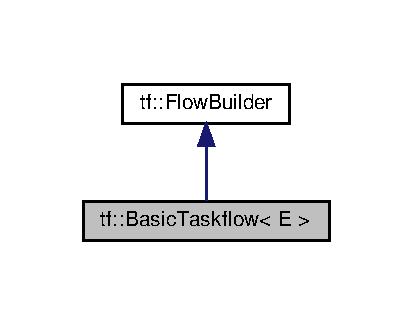
\includegraphics[width=198pt]{classtf_1_1BasicTaskflow__inherit__graph}
\end{center}
\end{figure}


Collaboration diagram for tf\+:\+:Basic\+Taskflow$<$ E $>$\+:\nopagebreak
\begin{figure}[H]
\begin{center}
\leavevmode
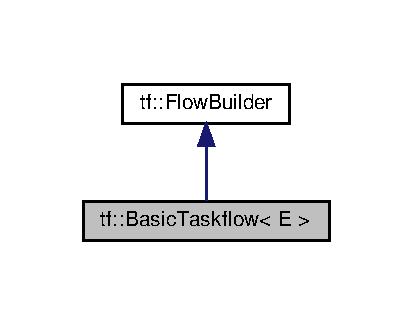
\includegraphics[width=198pt]{classtf_1_1BasicTaskflow__coll__graph}
\end{center}
\end{figure}
\subsection*{Public Types}
\begin{DoxyCompactItemize}
\item 
using \hyperlink{classtf_1_1BasicTaskflow_ab183cd063ba999ac62b5d4e9bb89247d}{Executor} = E$<$ Closure $>$
\end{DoxyCompactItemize}
\subsection*{Public Member Functions}
\begin{DoxyCompactItemize}
\item 
\hyperlink{classtf_1_1BasicTaskflow_ab077a9419b9cb6cbc9f9647c621c8c71}{Basic\+Taskflow} ()
\item 
\hyperlink{classtf_1_1BasicTaskflow_a005b6e5632ad3acd52406adf7d3e84e5}{Basic\+Taskflow} (unsigned)
\item 
\hyperlink{classtf_1_1BasicTaskflow_aa6301c0e9667a4a0ecd30f4d654ac135}{Basic\+Taskflow} (std\+::shared\+\_\+ptr$<$ \hyperlink{classtf_1_1BasicTaskflow_ab183cd063ba999ac62b5d4e9bb89247d}{Executor} $>$)
\item 
\hyperlink{classtf_1_1BasicTaskflow_ae820a9ab3cad471a591da4de749752ae}{$\sim$\+Basic\+Taskflow} ()
\item 
std\+::shared\+\_\+ptr$<$ \hyperlink{classtf_1_1BasicTaskflow_ab183cd063ba999ac62b5d4e9bb89247d}{Executor} $>$ \hyperlink{classtf_1_1BasicTaskflow_abe76e5288016861aaf1dafc0218d3084}{share\+\_\+executor} ()
\item 
std\+::shared\+\_\+future$<$ void $>$ \hyperlink{classtf_1_1BasicTaskflow_a848e425f67b49a8a7ac21f6b791999c5}{dispatch} ()
\item 
{\footnotesize template$<$typename C $>$ }\\std\+::shared\+\_\+future$<$ void $>$ \hyperlink{classtf_1_1BasicTaskflow_ae644520b734078d061e3ceafc7d982ad}{dispatch} (C \&\&)
\item 
void \hyperlink{classtf_1_1BasicTaskflow_a0126001a2bd8603af4827049578629cb}{silent\+\_\+dispatch} ()
\item 
{\footnotesize template$<$typename C $>$ }\\void \hyperlink{classtf_1_1BasicTaskflow_a8d27a4ec6768473a46460a39ba7c572c}{silent\+\_\+dispatch} (C \&\&)
\item 
void \hyperlink{classtf_1_1BasicTaskflow_a37ef86998f23ee7315be032c40fe815e}{wait\+\_\+for\+\_\+all} ()
\item 
void \hyperlink{classtf_1_1BasicTaskflow_a8f0ce2026118e97b83cbd727ed0932af}{wait\+\_\+for\+\_\+topologies} ()
\item 
void \hyperlink{classtf_1_1BasicTaskflow_aec75723fc4f48197bc92748ed8b12d2a}{dump} (std\+::ostream \&) const
\item 
void \hyperlink{classtf_1_1BasicTaskflow_a6ada71950f0e3384f2ab95814bbc7c3f}{dump\+\_\+topologies} (std\+::ostream \&) const
\item 
size\+\_\+t \hyperlink{classtf_1_1BasicTaskflow_a18341302575dcb719e455d84a738273f}{num\+\_\+nodes} () const
\item 
size\+\_\+t \hyperlink{classtf_1_1BasicTaskflow_a9cef9ee3d27ffc78bfa953c8ed25b559}{num\+\_\+workers} () const
\item 
size\+\_\+t \hyperlink{classtf_1_1BasicTaskflow_a7e97ed52d9d0470d2751f32748adb253}{num\+\_\+topologies} () const
\item 
std\+::string \hyperlink{classtf_1_1BasicTaskflow_a913a31040546bcf9d6e044580d170722}{dump} () const
\item 
std\+::string \hyperlink{classtf_1_1BasicTaskflow_ae4c67b7bc87564e8b5b309837f4b6d78}{dump\+\_\+topologies} () const
\end{DoxyCompactItemize}
\subsection*{Additional Inherited Members}


\subsection{Member Typedef Documentation}
\mbox{\Hypertarget{classtf_1_1BasicTaskflow_ab183cd063ba999ac62b5d4e9bb89247d}\label{classtf_1_1BasicTaskflow_ab183cd063ba999ac62b5d4e9bb89247d}} 
\index{tf\+::\+Basic\+Taskflow@{tf\+::\+Basic\+Taskflow}!Executor@{Executor}}
\index{Executor@{Executor}!tf\+::\+Basic\+Taskflow@{tf\+::\+Basic\+Taskflow}}
\subsubsection{\texorpdfstring{Executor}{Executor}}
{\footnotesize\ttfamily template$<$template$<$ typename... $>$ typename E$>$ \\
using \hyperlink{classtf_1_1BasicTaskflow}{tf\+::\+Basic\+Taskflow}$<$ E $>$\+::\hyperlink{classtf_1_1BasicTaskflow_ab183cd063ba999ac62b5d4e9bb89247d}{Executor} =  E$<$Closure$>$}



\subsection{Constructor \& Destructor Documentation}
\mbox{\Hypertarget{classtf_1_1BasicTaskflow_ab077a9419b9cb6cbc9f9647c621c8c71}\label{classtf_1_1BasicTaskflow_ab077a9419b9cb6cbc9f9647c621c8c71}} 
\index{tf\+::\+Basic\+Taskflow@{tf\+::\+Basic\+Taskflow}!Basic\+Taskflow@{Basic\+Taskflow}}
\index{Basic\+Taskflow@{Basic\+Taskflow}!tf\+::\+Basic\+Taskflow@{tf\+::\+Basic\+Taskflow}}
\subsubsection{\texorpdfstring{Basic\+Taskflow()}{BasicTaskflow()}\hspace{0.1cm}{\footnotesize\ttfamily [1/3]}}
{\footnotesize\ttfamily template$<$template$<$ typename... $>$ typename E$>$ \\
\hyperlink{classtf_1_1BasicTaskflow}{tf\+::\+Basic\+Taskflow}$<$ E $>$\+::\hyperlink{classtf_1_1BasicTaskflow}{Basic\+Taskflow} (\begin{DoxyParamCaption}{ }\end{DoxyParamCaption})\hspace{0.3cm}{\ttfamily [explicit]}}

\mbox{\Hypertarget{classtf_1_1BasicTaskflow_a005b6e5632ad3acd52406adf7d3e84e5}\label{classtf_1_1BasicTaskflow_a005b6e5632ad3acd52406adf7d3e84e5}} 
\index{tf\+::\+Basic\+Taskflow@{tf\+::\+Basic\+Taskflow}!Basic\+Taskflow@{Basic\+Taskflow}}
\index{Basic\+Taskflow@{Basic\+Taskflow}!tf\+::\+Basic\+Taskflow@{tf\+::\+Basic\+Taskflow}}
\subsubsection{\texorpdfstring{Basic\+Taskflow()}{BasicTaskflow()}\hspace{0.1cm}{\footnotesize\ttfamily [2/3]}}
{\footnotesize\ttfamily template$<$template$<$ typename... $>$ typename E$>$ \\
\hyperlink{classtf_1_1BasicTaskflow}{tf\+::\+Basic\+Taskflow}$<$ E $>$\+::\hyperlink{classtf_1_1BasicTaskflow}{Basic\+Taskflow} (\begin{DoxyParamCaption}\item[{unsigned}]{N }\end{DoxyParamCaption})\hspace{0.3cm}{\ttfamily [explicit]}}

\mbox{\Hypertarget{classtf_1_1BasicTaskflow_aa6301c0e9667a4a0ecd30f4d654ac135}\label{classtf_1_1BasicTaskflow_aa6301c0e9667a4a0ecd30f4d654ac135}} 
\index{tf\+::\+Basic\+Taskflow@{tf\+::\+Basic\+Taskflow}!Basic\+Taskflow@{Basic\+Taskflow}}
\index{Basic\+Taskflow@{Basic\+Taskflow}!tf\+::\+Basic\+Taskflow@{tf\+::\+Basic\+Taskflow}}
\subsubsection{\texorpdfstring{Basic\+Taskflow()}{BasicTaskflow()}\hspace{0.1cm}{\footnotesize\ttfamily [3/3]}}
{\footnotesize\ttfamily template$<$template$<$ typename... $>$ typename E$>$ \\
\hyperlink{classtf_1_1BasicTaskflow}{tf\+::\+Basic\+Taskflow}$<$ E $>$\+::\hyperlink{classtf_1_1BasicTaskflow}{Basic\+Taskflow} (\begin{DoxyParamCaption}\item[{std\+::shared\+\_\+ptr$<$ \hyperlink{classtf_1_1BasicTaskflow_ab183cd063ba999ac62b5d4e9bb89247d}{Executor} $>$}]{e }\end{DoxyParamCaption})\hspace{0.3cm}{\ttfamily [explicit]}}

\mbox{\Hypertarget{classtf_1_1BasicTaskflow_ae820a9ab3cad471a591da4de749752ae}\label{classtf_1_1BasicTaskflow_ae820a9ab3cad471a591da4de749752ae}} 
\index{tf\+::\+Basic\+Taskflow@{tf\+::\+Basic\+Taskflow}!````~Basic\+Taskflow@{$\sim$\+Basic\+Taskflow}}
\index{````~Basic\+Taskflow@{$\sim$\+Basic\+Taskflow}!tf\+::\+Basic\+Taskflow@{tf\+::\+Basic\+Taskflow}}
\subsubsection{\texorpdfstring{$\sim$\+Basic\+Taskflow()}{~BasicTaskflow()}}
{\footnotesize\ttfamily template$<$template$<$ typename... $>$ typename E$>$ \\
\hyperlink{classtf_1_1BasicTaskflow}{tf\+::\+Basic\+Taskflow}$<$ E $>$\+::$\sim$\hyperlink{classtf_1_1BasicTaskflow}{Basic\+Taskflow} (\begin{DoxyParamCaption}{ }\end{DoxyParamCaption})}



\subsection{Member Function Documentation}
\mbox{\Hypertarget{classtf_1_1BasicTaskflow_a848e425f67b49a8a7ac21f6b791999c5}\label{classtf_1_1BasicTaskflow_a848e425f67b49a8a7ac21f6b791999c5}} 
\index{tf\+::\+Basic\+Taskflow@{tf\+::\+Basic\+Taskflow}!dispatch@{dispatch}}
\index{dispatch@{dispatch}!tf\+::\+Basic\+Taskflow@{tf\+::\+Basic\+Taskflow}}
\subsubsection{\texorpdfstring{dispatch()}{dispatch()}\hspace{0.1cm}{\footnotesize\ttfamily [1/2]}}
{\footnotesize\ttfamily template$<$template$<$ typename... $>$ typename E$>$ \\
std\+::shared\+\_\+future$<$ void $>$ \hyperlink{classtf_1_1BasicTaskflow}{tf\+::\+Basic\+Taskflow}$<$ E $>$\+::dispatch (\begin{DoxyParamCaption}{ }\end{DoxyParamCaption})}

\mbox{\Hypertarget{classtf_1_1BasicTaskflow_ae644520b734078d061e3ceafc7d982ad}\label{classtf_1_1BasicTaskflow_ae644520b734078d061e3ceafc7d982ad}} 
\index{tf\+::\+Basic\+Taskflow@{tf\+::\+Basic\+Taskflow}!dispatch@{dispatch}}
\index{dispatch@{dispatch}!tf\+::\+Basic\+Taskflow@{tf\+::\+Basic\+Taskflow}}
\subsubsection{\texorpdfstring{dispatch()}{dispatch()}\hspace{0.1cm}{\footnotesize\ttfamily [2/2]}}
{\footnotesize\ttfamily template$<$template$<$ typename... $>$ typename E$>$ \\
template$<$typename C $>$ \\
std\+::shared\+\_\+future$<$ void $>$ \hyperlink{classtf_1_1BasicTaskflow}{tf\+::\+Basic\+Taskflow}$<$ E $>$\+::dispatch (\begin{DoxyParamCaption}\item[{C \&\&}]{c }\end{DoxyParamCaption})}

\mbox{\Hypertarget{classtf_1_1BasicTaskflow_aec75723fc4f48197bc92748ed8b12d2a}\label{classtf_1_1BasicTaskflow_aec75723fc4f48197bc92748ed8b12d2a}} 
\index{tf\+::\+Basic\+Taskflow@{tf\+::\+Basic\+Taskflow}!dump@{dump}}
\index{dump@{dump}!tf\+::\+Basic\+Taskflow@{tf\+::\+Basic\+Taskflow}}
\subsubsection{\texorpdfstring{dump()}{dump()}\hspace{0.1cm}{\footnotesize\ttfamily [1/2]}}
{\footnotesize\ttfamily template$<$template$<$ typename... $>$ typename E$>$ \\
void \hyperlink{classtf_1_1BasicTaskflow}{tf\+::\+Basic\+Taskflow}$<$ E $>$\+::dump (\begin{DoxyParamCaption}\item[{std\+::ostream \&}]{os }\end{DoxyParamCaption}) const}

\mbox{\Hypertarget{classtf_1_1BasicTaskflow_a913a31040546bcf9d6e044580d170722}\label{classtf_1_1BasicTaskflow_a913a31040546bcf9d6e044580d170722}} 
\index{tf\+::\+Basic\+Taskflow@{tf\+::\+Basic\+Taskflow}!dump@{dump}}
\index{dump@{dump}!tf\+::\+Basic\+Taskflow@{tf\+::\+Basic\+Taskflow}}
\subsubsection{\texorpdfstring{dump()}{dump()}\hspace{0.1cm}{\footnotesize\ttfamily [2/2]}}
{\footnotesize\ttfamily template$<$template$<$ typename... $>$ typename E$>$ \\
std\+::string \hyperlink{classtf_1_1BasicTaskflow}{tf\+::\+Basic\+Taskflow}$<$ E $>$\+::dump (\begin{DoxyParamCaption}{ }\end{DoxyParamCaption}) const}

\mbox{\Hypertarget{classtf_1_1BasicTaskflow_a6ada71950f0e3384f2ab95814bbc7c3f}\label{classtf_1_1BasicTaskflow_a6ada71950f0e3384f2ab95814bbc7c3f}} 
\index{tf\+::\+Basic\+Taskflow@{tf\+::\+Basic\+Taskflow}!dump\+\_\+topologies@{dump\+\_\+topologies}}
\index{dump\+\_\+topologies@{dump\+\_\+topologies}!tf\+::\+Basic\+Taskflow@{tf\+::\+Basic\+Taskflow}}
\subsubsection{\texorpdfstring{dump\+\_\+topologies()}{dump\_topologies()}\hspace{0.1cm}{\footnotesize\ttfamily [1/2]}}
{\footnotesize\ttfamily template$<$template$<$ typename... $>$ typename E$>$ \\
void \hyperlink{classtf_1_1BasicTaskflow}{tf\+::\+Basic\+Taskflow}$<$ E $>$\+::dump\+\_\+topologies (\begin{DoxyParamCaption}\item[{std\+::ostream \&}]{os }\end{DoxyParamCaption}) const}

\mbox{\Hypertarget{classtf_1_1BasicTaskflow_ae4c67b7bc87564e8b5b309837f4b6d78}\label{classtf_1_1BasicTaskflow_ae4c67b7bc87564e8b5b309837f4b6d78}} 
\index{tf\+::\+Basic\+Taskflow@{tf\+::\+Basic\+Taskflow}!dump\+\_\+topologies@{dump\+\_\+topologies}}
\index{dump\+\_\+topologies@{dump\+\_\+topologies}!tf\+::\+Basic\+Taskflow@{tf\+::\+Basic\+Taskflow}}
\subsubsection{\texorpdfstring{dump\+\_\+topologies()}{dump\_topologies()}\hspace{0.1cm}{\footnotesize\ttfamily [2/2]}}
{\footnotesize\ttfamily template$<$template$<$ typename... $>$ typename E$>$ \\
std\+::string \hyperlink{classtf_1_1BasicTaskflow}{tf\+::\+Basic\+Taskflow}$<$ E $>$\+::dump\+\_\+topologies (\begin{DoxyParamCaption}{ }\end{DoxyParamCaption}) const}

\mbox{\Hypertarget{classtf_1_1BasicTaskflow_a18341302575dcb719e455d84a738273f}\label{classtf_1_1BasicTaskflow_a18341302575dcb719e455d84a738273f}} 
\index{tf\+::\+Basic\+Taskflow@{tf\+::\+Basic\+Taskflow}!num\+\_\+nodes@{num\+\_\+nodes}}
\index{num\+\_\+nodes@{num\+\_\+nodes}!tf\+::\+Basic\+Taskflow@{tf\+::\+Basic\+Taskflow}}
\subsubsection{\texorpdfstring{num\+\_\+nodes()}{num\_nodes()}}
{\footnotesize\ttfamily template$<$template$<$ typename... $>$ typename E$>$ \\
size\+\_\+t \hyperlink{classtf_1_1BasicTaskflow}{tf\+::\+Basic\+Taskflow}$<$ E $>$\+::num\+\_\+nodes (\begin{DoxyParamCaption}{ }\end{DoxyParamCaption}) const}

\mbox{\Hypertarget{classtf_1_1BasicTaskflow_a7e97ed52d9d0470d2751f32748adb253}\label{classtf_1_1BasicTaskflow_a7e97ed52d9d0470d2751f32748adb253}} 
\index{tf\+::\+Basic\+Taskflow@{tf\+::\+Basic\+Taskflow}!num\+\_\+topologies@{num\+\_\+topologies}}
\index{num\+\_\+topologies@{num\+\_\+topologies}!tf\+::\+Basic\+Taskflow@{tf\+::\+Basic\+Taskflow}}
\subsubsection{\texorpdfstring{num\+\_\+topologies()}{num\_topologies()}}
{\footnotesize\ttfamily template$<$template$<$ typename... $>$ typename E$>$ \\
size\+\_\+t \hyperlink{classtf_1_1BasicTaskflow}{tf\+::\+Basic\+Taskflow}$<$ E $>$\+::num\+\_\+topologies (\begin{DoxyParamCaption}{ }\end{DoxyParamCaption}) const}

\mbox{\Hypertarget{classtf_1_1BasicTaskflow_a9cef9ee3d27ffc78bfa953c8ed25b559}\label{classtf_1_1BasicTaskflow_a9cef9ee3d27ffc78bfa953c8ed25b559}} 
\index{tf\+::\+Basic\+Taskflow@{tf\+::\+Basic\+Taskflow}!num\+\_\+workers@{num\+\_\+workers}}
\index{num\+\_\+workers@{num\+\_\+workers}!tf\+::\+Basic\+Taskflow@{tf\+::\+Basic\+Taskflow}}
\subsubsection{\texorpdfstring{num\+\_\+workers()}{num\_workers()}}
{\footnotesize\ttfamily template$<$template$<$ typename... $>$ typename E$>$ \\
size\+\_\+t \hyperlink{classtf_1_1BasicTaskflow}{tf\+::\+Basic\+Taskflow}$<$ E $>$\+::num\+\_\+workers (\begin{DoxyParamCaption}{ }\end{DoxyParamCaption}) const}

\mbox{\Hypertarget{classtf_1_1BasicTaskflow_abe76e5288016861aaf1dafc0218d3084}\label{classtf_1_1BasicTaskflow_abe76e5288016861aaf1dafc0218d3084}} 
\index{tf\+::\+Basic\+Taskflow@{tf\+::\+Basic\+Taskflow}!share\+\_\+executor@{share\+\_\+executor}}
\index{share\+\_\+executor@{share\+\_\+executor}!tf\+::\+Basic\+Taskflow@{tf\+::\+Basic\+Taskflow}}
\subsubsection{\texorpdfstring{share\+\_\+executor()}{share\_executor()}}
{\footnotesize\ttfamily template$<$template$<$ typename... $>$ typename E$>$ \\
std\+::shared\+\_\+ptr$<$ typename \hyperlink{classtf_1_1BasicTaskflow}{Basic\+Taskflow}$<$ E $>$\+::\hyperlink{classtf_1_1BasicTaskflow_ab183cd063ba999ac62b5d4e9bb89247d}{Executor} $>$ \hyperlink{classtf_1_1BasicTaskflow}{tf\+::\+Basic\+Taskflow}$<$ E $>$\+::share\+\_\+executor (\begin{DoxyParamCaption}{ }\end{DoxyParamCaption})}

\mbox{\Hypertarget{classtf_1_1BasicTaskflow_a0126001a2bd8603af4827049578629cb}\label{classtf_1_1BasicTaskflow_a0126001a2bd8603af4827049578629cb}} 
\index{tf\+::\+Basic\+Taskflow@{tf\+::\+Basic\+Taskflow}!silent\+\_\+dispatch@{silent\+\_\+dispatch}}
\index{silent\+\_\+dispatch@{silent\+\_\+dispatch}!tf\+::\+Basic\+Taskflow@{tf\+::\+Basic\+Taskflow}}
\subsubsection{\texorpdfstring{silent\+\_\+dispatch()}{silent\_dispatch()}\hspace{0.1cm}{\footnotesize\ttfamily [1/2]}}
{\footnotesize\ttfamily template$<$template$<$ typename... $>$ typename E$>$ \\
void \hyperlink{classtf_1_1BasicTaskflow}{tf\+::\+Basic\+Taskflow}$<$ E $>$\+::silent\+\_\+dispatch (\begin{DoxyParamCaption}{ }\end{DoxyParamCaption})}

\mbox{\Hypertarget{classtf_1_1BasicTaskflow_a8d27a4ec6768473a46460a39ba7c572c}\label{classtf_1_1BasicTaskflow_a8d27a4ec6768473a46460a39ba7c572c}} 
\index{tf\+::\+Basic\+Taskflow@{tf\+::\+Basic\+Taskflow}!silent\+\_\+dispatch@{silent\+\_\+dispatch}}
\index{silent\+\_\+dispatch@{silent\+\_\+dispatch}!tf\+::\+Basic\+Taskflow@{tf\+::\+Basic\+Taskflow}}
\subsubsection{\texorpdfstring{silent\+\_\+dispatch()}{silent\_dispatch()}\hspace{0.1cm}{\footnotesize\ttfamily [2/2]}}
{\footnotesize\ttfamily template$<$template$<$ typename... $>$ typename E$>$ \\
template$<$typename C $>$ \\
void \hyperlink{classtf_1_1BasicTaskflow}{tf\+::\+Basic\+Taskflow}$<$ E $>$\+::silent\+\_\+dispatch (\begin{DoxyParamCaption}\item[{C \&\&}]{c }\end{DoxyParamCaption})}

\mbox{\Hypertarget{classtf_1_1BasicTaskflow_a37ef86998f23ee7315be032c40fe815e}\label{classtf_1_1BasicTaskflow_a37ef86998f23ee7315be032c40fe815e}} 
\index{tf\+::\+Basic\+Taskflow@{tf\+::\+Basic\+Taskflow}!wait\+\_\+for\+\_\+all@{wait\+\_\+for\+\_\+all}}
\index{wait\+\_\+for\+\_\+all@{wait\+\_\+for\+\_\+all}!tf\+::\+Basic\+Taskflow@{tf\+::\+Basic\+Taskflow}}
\subsubsection{\texorpdfstring{wait\+\_\+for\+\_\+all()}{wait\_for\_all()}}
{\footnotesize\ttfamily template$<$template$<$ typename... $>$ typename E$>$ \\
void \hyperlink{classtf_1_1BasicTaskflow}{tf\+::\+Basic\+Taskflow}$<$ E $>$\+::wait\+\_\+for\+\_\+all (\begin{DoxyParamCaption}{ }\end{DoxyParamCaption})}

\mbox{\Hypertarget{classtf_1_1BasicTaskflow_a8f0ce2026118e97b83cbd727ed0932af}\label{classtf_1_1BasicTaskflow_a8f0ce2026118e97b83cbd727ed0932af}} 
\index{tf\+::\+Basic\+Taskflow@{tf\+::\+Basic\+Taskflow}!wait\+\_\+for\+\_\+topologies@{wait\+\_\+for\+\_\+topologies}}
\index{wait\+\_\+for\+\_\+topologies@{wait\+\_\+for\+\_\+topologies}!tf\+::\+Basic\+Taskflow@{tf\+::\+Basic\+Taskflow}}
\subsubsection{\texorpdfstring{wait\+\_\+for\+\_\+topologies()}{wait\_for\_topologies()}}
{\footnotesize\ttfamily template$<$template$<$ typename... $>$ typename E$>$ \\
void \hyperlink{classtf_1_1BasicTaskflow}{tf\+::\+Basic\+Taskflow}$<$ E $>$\+::wait\+\_\+for\+\_\+topologies (\begin{DoxyParamCaption}{ }\end{DoxyParamCaption})}



The documentation for this class was generated from the following file\+:\begin{DoxyCompactItemize}
\item 
/home/twhuang/\+Ph\+D/\+Code/cpp-\/taskflow/taskflow/graph/\hyperlink{basic__taskflow_8hpp}{basic\+\_\+taskflow.\+hpp}\end{DoxyCompactItemize}

\hypertarget{structtf_1_1dependent__false}{}\section{tf\+:\+:dependent\+\_\+false$<$ T $>$ Struct Template Reference}
\label{structtf_1_1dependent__false}\index{tf\+::dependent\+\_\+false$<$ T $>$@{tf\+::dependent\+\_\+false$<$ T $>$}}


{\ttfamily \#include $<$utility.\+hpp$>$}

\subsection*{Static Public Attributes}
\begin{DoxyCompactItemize}
\item 
static constexpr bool \hyperlink{structtf_1_1dependent__false_a84f8288ae187aa71e02e51d9d3f0b328}{value} = false
\end{DoxyCompactItemize}


\subsection{Member Data Documentation}
\mbox{\Hypertarget{structtf_1_1dependent__false_a84f8288ae187aa71e02e51d9d3f0b328}\label{structtf_1_1dependent__false_a84f8288ae187aa71e02e51d9d3f0b328}} 
\index{tf\+::dependent\+\_\+false@{tf\+::dependent\+\_\+false}!value@{value}}
\index{value@{value}!tf\+::dependent\+\_\+false@{tf\+::dependent\+\_\+false}}
\subsubsection{\texorpdfstring{value}{value}}
{\footnotesize\ttfamily template$<$typename... T$>$ \\
constexpr bool \hyperlink{structtf_1_1dependent__false}{tf\+::dependent\+\_\+false}$<$ T $>$\+::value = false\hspace{0.3cm}{\ttfamily [static]}}



The documentation for this struct was generated from the following file\+:\begin{DoxyCompactItemize}
\item 
/home/twhuang/\+Ph\+D/\+Code/cpp-\/taskflow/taskflow/utility/\hyperlink{utility_8hpp}{utility.\+hpp}\end{DoxyCompactItemize}

\hypertarget{structtf_1_1Error}{}\section{tf\+:\+:Error Struct Reference}
\label{structtf_1_1Error}\index{tf\+::\+Error@{tf\+::\+Error}}


{\ttfamily \#include $<$error.\+hpp$>$}



Inheritance diagram for tf\+:\+:Error\+:\nopagebreak
\begin{figure}[H]
\begin{center}
\leavevmode
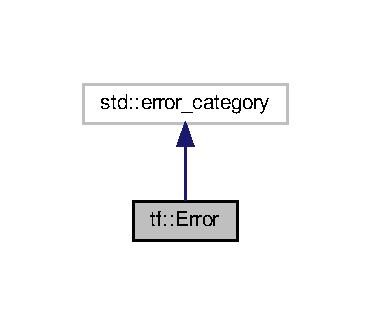
\includegraphics[width=178pt]{structtf_1_1Error__inherit__graph}
\end{center}
\end{figure}


Collaboration diagram for tf\+:\+:Error\+:\nopagebreak
\begin{figure}[H]
\begin{center}
\leavevmode
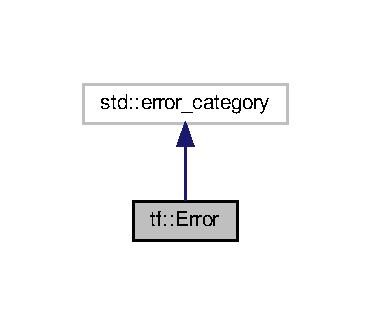
\includegraphics[width=178pt]{structtf_1_1Error__coll__graph}
\end{center}
\end{figure}
\subsection*{Public Types}
\begin{DoxyCompactItemize}
\item 
enum \hyperlink{structtf_1_1Error_aad6732b815bfe4ae3cea402042ee43a3}{Code} \+: int \{ \hyperlink{structtf_1_1Error_aad6732b815bfe4ae3cea402042ee43a3acfa4fd6143c71e68422b942ea4137bd8}{S\+U\+C\+C\+E\+SS} = 0, 
\hyperlink{structtf_1_1Error_aad6732b815bfe4ae3cea402042ee43a3a473f4090f21daf6a44dfa954277922d0}{F\+L\+O\+W\+\_\+\+B\+U\+I\+L\+D\+ER}, 
\hyperlink{structtf_1_1Error_aad6732b815bfe4ae3cea402042ee43a3a55ebe8318d63f4c36ae93b0ec26dc9b2}{E\+X\+E\+C\+U\+T\+OR}
 \}
\end{DoxyCompactItemize}
\subsection*{Public Member Functions}
\begin{DoxyCompactItemize}
\item 
const char $\ast$ \hyperlink{structtf_1_1Error_a18a5c2f16b543d5361e8a24554ebd12c}{name} () const noexcept override final
\item 
std\+::string \hyperlink{structtf_1_1Error_ae2d8630128262023502664f3cae5daab}{message} (int) const override final
\end{DoxyCompactItemize}
\subsection*{Static Public Member Functions}
\begin{DoxyCompactItemize}
\item 
static const std\+::error\+\_\+category \& \hyperlink{structtf_1_1Error_a2fdb64a058ea1ff03706d0cd69c36021}{get} ()
\end{DoxyCompactItemize}


\subsection{Member Enumeration Documentation}
\mbox{\Hypertarget{structtf_1_1Error_aad6732b815bfe4ae3cea402042ee43a3}\label{structtf_1_1Error_aad6732b815bfe4ae3cea402042ee43a3}} 
\index{tf\+::\+Error@{tf\+::\+Error}!Code@{Code}}
\index{Code@{Code}!tf\+::\+Error@{tf\+::\+Error}}
\subsubsection{\texorpdfstring{Code}{Code}}
{\footnotesize\ttfamily enum \hyperlink{structtf_1_1Error_aad6732b815bfe4ae3cea402042ee43a3}{tf\+::\+Error\+::\+Code} \+: int}

\begin{DoxyEnumFields}{Enumerator}
\raisebox{\heightof{T}}[0pt][0pt]{\index{S\+U\+C\+C\+E\+SS@{S\+U\+C\+C\+E\+SS}!tf\+::\+Error@{tf\+::\+Error}}\index{tf\+::\+Error@{tf\+::\+Error}!S\+U\+C\+C\+E\+SS@{S\+U\+C\+C\+E\+SS}}}\mbox{\Hypertarget{structtf_1_1Error_aad6732b815bfe4ae3cea402042ee43a3acfa4fd6143c71e68422b942ea4137bd8}\label{structtf_1_1Error_aad6732b815bfe4ae3cea402042ee43a3acfa4fd6143c71e68422b942ea4137bd8}} 
S\+U\+C\+C\+E\+SS&\\
\hline

\raisebox{\heightof{T}}[0pt][0pt]{\index{F\+L\+O\+W\+\_\+\+B\+U\+I\+L\+D\+ER@{F\+L\+O\+W\+\_\+\+B\+U\+I\+L\+D\+ER}!tf\+::\+Error@{tf\+::\+Error}}\index{tf\+::\+Error@{tf\+::\+Error}!F\+L\+O\+W\+\_\+\+B\+U\+I\+L\+D\+ER@{F\+L\+O\+W\+\_\+\+B\+U\+I\+L\+D\+ER}}}\mbox{\Hypertarget{structtf_1_1Error_aad6732b815bfe4ae3cea402042ee43a3a473f4090f21daf6a44dfa954277922d0}\label{structtf_1_1Error_aad6732b815bfe4ae3cea402042ee43a3a473f4090f21daf6a44dfa954277922d0}} 
F\+L\+O\+W\+\_\+\+B\+U\+I\+L\+D\+ER&\\
\hline

\raisebox{\heightof{T}}[0pt][0pt]{\index{E\+X\+E\+C\+U\+T\+OR@{E\+X\+E\+C\+U\+T\+OR}!tf\+::\+Error@{tf\+::\+Error}}\index{tf\+::\+Error@{tf\+::\+Error}!E\+X\+E\+C\+U\+T\+OR@{E\+X\+E\+C\+U\+T\+OR}}}\mbox{\Hypertarget{structtf_1_1Error_aad6732b815bfe4ae3cea402042ee43a3a55ebe8318d63f4c36ae93b0ec26dc9b2}\label{structtf_1_1Error_aad6732b815bfe4ae3cea402042ee43a3a55ebe8318d63f4c36ae93b0ec26dc9b2}} 
E\+X\+E\+C\+U\+T\+OR&\\
\hline

\end{DoxyEnumFields}


\subsection{Member Function Documentation}
\mbox{\Hypertarget{structtf_1_1Error_a2fdb64a058ea1ff03706d0cd69c36021}\label{structtf_1_1Error_a2fdb64a058ea1ff03706d0cd69c36021}} 
\index{tf\+::\+Error@{tf\+::\+Error}!get@{get}}
\index{get@{get}!tf\+::\+Error@{tf\+::\+Error}}
\subsubsection{\texorpdfstring{get()}{get()}}
{\footnotesize\ttfamily const std\+::error\+\_\+category \& tf\+::\+Error\+::get (\begin{DoxyParamCaption}{ }\end{DoxyParamCaption})\hspace{0.3cm}{\ttfamily [inline]}, {\ttfamily [static]}}

\mbox{\Hypertarget{structtf_1_1Error_ae2d8630128262023502664f3cae5daab}\label{structtf_1_1Error_ae2d8630128262023502664f3cae5daab}} 
\index{tf\+::\+Error@{tf\+::\+Error}!message@{message}}
\index{message@{message}!tf\+::\+Error@{tf\+::\+Error}}
\subsubsection{\texorpdfstring{message()}{message()}}
{\footnotesize\ttfamily std\+::string tf\+::\+Error\+::message (\begin{DoxyParamCaption}\item[{int}]{code }\end{DoxyParamCaption}) const\hspace{0.3cm}{\ttfamily [inline]}, {\ttfamily [final]}, {\ttfamily [override]}}

\mbox{\Hypertarget{structtf_1_1Error_a18a5c2f16b543d5361e8a24554ebd12c}\label{structtf_1_1Error_a18a5c2f16b543d5361e8a24554ebd12c}} 
\index{tf\+::\+Error@{tf\+::\+Error}!name@{name}}
\index{name@{name}!tf\+::\+Error@{tf\+::\+Error}}
\subsubsection{\texorpdfstring{name()}{name()}}
{\footnotesize\ttfamily const char $\ast$ tf\+::\+Error\+::name (\begin{DoxyParamCaption}{ }\end{DoxyParamCaption}) const\hspace{0.3cm}{\ttfamily [inline]}, {\ttfamily [final]}, {\ttfamily [override]}, {\ttfamily [noexcept]}}



The documentation for this struct was generated from the following file\+:\begin{DoxyCompactItemize}
\item 
/home/twhuang/\+Ph\+D/\+Code/cpp-\/taskflow/taskflow/error/\hyperlink{error_8hpp}{error.\+hpp}\end{DoxyCompactItemize}

\hypertarget{classtf_1_1FlowBuilder}{}\section{tf\+:\+:Flow\+Builder Class Reference}
\label{classtf_1_1FlowBuilder}\index{tf\+::\+Flow\+Builder@{tf\+::\+Flow\+Builder}}


{\ttfamily \#include $<$flow\+\_\+builder.\+hpp$>$}



Inheritance diagram for tf\+:\+:Flow\+Builder\+:\nopagebreak
\begin{figure}[H]
\begin{center}
\leavevmode
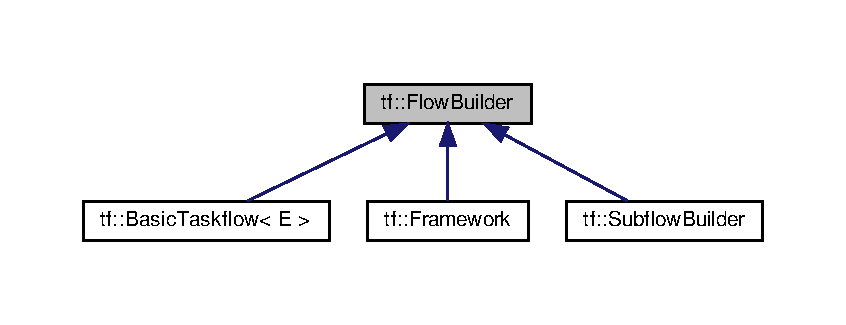
\includegraphics[width=350pt]{classtf_1_1FlowBuilder__inherit__graph}
\end{center}
\end{figure}
\subsection*{Public Member Functions}
\begin{DoxyCompactItemize}
\item 
\hyperlink{classtf_1_1FlowBuilder_ab9fcccd3c62467052a263b2fd2ca406b}{Flow\+Builder} (\hyperlink{namespacetf_a2afa7da139285640eaf8122535136dc9}{Graph} \&)
\item 
{\footnotesize template$<$typename C $>$ }\\auto \hyperlink{classtf_1_1FlowBuilder_a6d9c6008100d099994362769d1ea7fbb}{emplace} (C \&\&)
\item 
{\footnotesize template$<$typename... C, std\+::enable\+\_\+if\+\_\+t$<$(sizeof...(\+C)$>$ 1$>$ }\\auto \hyperlink{classtf_1_1FlowBuilder_ac4ccd002efe1e62a328632ce704bcd7a}{emplace} (C \&\&...)
\item 
{\footnotesize template$<$typename C $>$ }\\auto \hyperlink{classtf_1_1FlowBuilder_af8cdada0684ce221c4c134e1504cabd6}{silent\+\_\+emplace} (C \&\&)
\item 
{\footnotesize template$<$typename... C, std\+::enable\+\_\+if\+\_\+t$<$(sizeof...(\+C)$>$ 1$>$ }\\auto \hyperlink{classtf_1_1FlowBuilder_ad313d46679d6e38c361dbe13c28cebf6}{silent\+\_\+emplace} (C \&\&...)
\item 
{\footnotesize template$<$typename I , typename C $>$ }\\auto \hyperlink{classtf_1_1FlowBuilder_a016f6bb3fd6719eda5211c7befab3830}{parallel\+\_\+for} (I, I, C \&\&, size\+\_\+t=0)
\item 
{\footnotesize template$<$typename T , typename C , std\+::enable\+\_\+if\+\_\+t$<$ is\+\_\+iterable\+\_\+v$<$ T $>$, void $>$ $\ast$  = nullptr$>$ }\\auto \hyperlink{classtf_1_1FlowBuilder_a688d084ec1b29c78405a07d40cddd03c}{parallel\+\_\+for} (T \&, C \&\&, size\+\_\+t=0)
\item 
{\footnotesize template$<$typename I , typename C , std\+::enable\+\_\+if\+\_\+t$<$ std\+::is\+\_\+arithmetic\+\_\+v$<$ I $>$, void $>$ $\ast$  = nullptr$>$ }\\auto \hyperlink{classtf_1_1FlowBuilder_a54836d5d8b01e2732ad80091d9f50c18}{parallel\+\_\+for} (I, I, I, C \&\&, size\+\_\+t=0)
\item 
{\footnotesize template$<$typename I , typename T , typename B $>$ }\\auto \hyperlink{classtf_1_1FlowBuilder_a977deae532c85dca046658a0048daa8e}{reduce} (I, I, T \&, B \&\&)
\item 
{\footnotesize template$<$typename I , typename T $>$ }\\auto \hyperlink{classtf_1_1FlowBuilder_a3b1c5cb2d1ffd721662aa6b085fe7622}{reduce\+\_\+min} (I, I, T \&)
\item 
{\footnotesize template$<$typename I , typename T $>$ }\\auto \hyperlink{classtf_1_1FlowBuilder_aed9365d31c3f897cf5c45fb7ea917aa1}{reduce\+\_\+max} (I, I, T \&)
\item 
{\footnotesize template$<$typename I , typename T , typename B , typename U $>$ }\\auto \hyperlink{classtf_1_1FlowBuilder_ac4d38ee88ae922d3cb8c9808c418764f}{transform\+\_\+reduce} (I, I, T \&, B \&\&, U \&\&)
\item 
{\footnotesize template$<$typename I , typename T , typename B , typename P , typename U $>$ }\\auto \hyperlink{classtf_1_1FlowBuilder_a7bf4ad06f14f95bbc886ee087773712a}{transform\+\_\+reduce} (I, I, T \&, B \&\&, P \&\&, U \&\&)
\item 
auto \hyperlink{classtf_1_1FlowBuilder_ac22f244fb2ec58809192faafa266c58c}{placeholder} ()
\item 
void \hyperlink{classtf_1_1FlowBuilder_a6888a33d7b1a6df27b502f5dc736305e}{precede} (\hyperlink{classtf_1_1Task}{Task}, \hyperlink{classtf_1_1Task}{Task})
\item 
void \hyperlink{classtf_1_1FlowBuilder_a830e6242588432bac68c4430ae5912f6}{linearize} (std\+::vector$<$ \hyperlink{classtf_1_1Task}{Task} $>$ \&)
\item 
void \hyperlink{classtf_1_1FlowBuilder_a2844c99c971f223ddeeba4f2bb6694f9}{linearize} (std\+::initializer\+\_\+list$<$ \hyperlink{classtf_1_1Task}{Task} $>$)
\item 
void \hyperlink{classtf_1_1FlowBuilder_a300450cb88280bf485c6706da5233690}{broadcast} (\hyperlink{classtf_1_1Task}{Task}, std\+::vector$<$ \hyperlink{classtf_1_1Task}{Task} $>$ \&)
\item 
void \hyperlink{classtf_1_1FlowBuilder_a0472082e25fbc1528cef5ba55f096fc4}{broadcast} (\hyperlink{classtf_1_1Task}{Task}, std\+::initializer\+\_\+list$<$ \hyperlink{classtf_1_1Task}{Task} $>$)
\item 
void \hyperlink{classtf_1_1FlowBuilder_a6f68be7b9cf49770abbbc2b1fcb4d461}{gather} (std\+::vector$<$ \hyperlink{classtf_1_1Task}{Task} $>$ \&, \hyperlink{classtf_1_1Task}{Task})
\item 
void \hyperlink{classtf_1_1FlowBuilder_a96c59ed5cdab83efd7e4a42f81241e69}{gather} (std\+::initializer\+\_\+list$<$ \hyperlink{classtf_1_1Task}{Task} $>$, \hyperlink{classtf_1_1Task}{Task})
\item 
size\+\_\+t \hyperlink{classtf_1_1FlowBuilder_ab0f3d86726d6e803dedeb2811bf811c3}{size} () const
\item 
bool \hyperlink{classtf_1_1FlowBuilder_a18909c48304f1827884708dc943efb6a}{empty} () const
\item 
{\footnotesize template$<$typename... C, std\+::enable\+\_\+if\+\_\+t$<$(sizeof...(\+C)$>$ 1$>$ }\\auto \hyperlink{classtf_1_1FlowBuilder_abe0b13ab3bb54903c6ea6856101aae5b}{silent\+\_\+emplace} (C \&\&... cs)
\item 
{\footnotesize template$<$typename... C, std\+::enable\+\_\+if\+\_\+t$<$(sizeof...(\+C)$>$ 1$>$ }\\auto \hyperlink{classtf_1_1FlowBuilder_aaf1c2bad2e5f31225584db88019a952a}{emplace} (C \&\&... cs)
\end{DoxyCompactItemize}
\subsection*{Protected Member Functions}
\begin{DoxyCompactItemize}
\item 
{\footnotesize template$<$typename L $>$ }\\void \hyperlink{classtf_1_1FlowBuilder_a04115519f61efc42d018ea697054135d}{\+\_\+linearize} (L \&)
\item 
{\footnotesize template$<$typename I $>$ }\\size\+\_\+t \hyperlink{classtf_1_1FlowBuilder_ab98b07f1f11153628d1e1222058e9b55}{\+\_\+estimate\+\_\+chunk\+\_\+size} (I, I, I)
\end{DoxyCompactItemize}
\subsection*{Protected Attributes}
\begin{DoxyCompactItemize}
\item 
\hyperlink{namespacetf_a2afa7da139285640eaf8122535136dc9}{Graph} \& \hyperlink{classtf_1_1FlowBuilder_a9404a57d9d37a4d49d20b686e4e5f68f}{\+\_\+graph}
\end{DoxyCompactItemize}


\subsection{Constructor \& Destructor Documentation}
\mbox{\Hypertarget{classtf_1_1FlowBuilder_ab9fcccd3c62467052a263b2fd2ca406b}\label{classtf_1_1FlowBuilder_ab9fcccd3c62467052a263b2fd2ca406b}} 
\index{tf\+::\+Flow\+Builder@{tf\+::\+Flow\+Builder}!Flow\+Builder@{Flow\+Builder}}
\index{Flow\+Builder@{Flow\+Builder}!tf\+::\+Flow\+Builder@{tf\+::\+Flow\+Builder}}
\subsubsection{\texorpdfstring{Flow\+Builder()}{FlowBuilder()}}
{\footnotesize\ttfamily tf\+::\+Flow\+Builder\+::\+Flow\+Builder (\begin{DoxyParamCaption}\item[{\hyperlink{namespacetf_a2afa7da139285640eaf8122535136dc9}{Graph} \&}]{graph }\end{DoxyParamCaption})\hspace{0.3cm}{\ttfamily [inline]}}



\subsection{Member Function Documentation}
\mbox{\Hypertarget{classtf_1_1FlowBuilder_ab98b07f1f11153628d1e1222058e9b55}\label{classtf_1_1FlowBuilder_ab98b07f1f11153628d1e1222058e9b55}} 
\index{tf\+::\+Flow\+Builder@{tf\+::\+Flow\+Builder}!\+\_\+estimate\+\_\+chunk\+\_\+size@{\+\_\+estimate\+\_\+chunk\+\_\+size}}
\index{\+\_\+estimate\+\_\+chunk\+\_\+size@{\+\_\+estimate\+\_\+chunk\+\_\+size}!tf\+::\+Flow\+Builder@{tf\+::\+Flow\+Builder}}
\subsubsection{\texorpdfstring{\+\_\+estimate\+\_\+chunk\+\_\+size()}{\_estimate\_chunk\_size()}}
{\footnotesize\ttfamily template$<$typename I $>$ \\
size\+\_\+t tf\+::\+Flow\+Builder\+::\+\_\+estimate\+\_\+chunk\+\_\+size (\begin{DoxyParamCaption}\item[{I}]{beg,  }\item[{I}]{end,  }\item[{I}]{step }\end{DoxyParamCaption})\hspace{0.3cm}{\ttfamily [protected]}}

\mbox{\Hypertarget{classtf_1_1FlowBuilder_a04115519f61efc42d018ea697054135d}\label{classtf_1_1FlowBuilder_a04115519f61efc42d018ea697054135d}} 
\index{tf\+::\+Flow\+Builder@{tf\+::\+Flow\+Builder}!\+\_\+linearize@{\+\_\+linearize}}
\index{\+\_\+linearize@{\+\_\+linearize}!tf\+::\+Flow\+Builder@{tf\+::\+Flow\+Builder}}
\subsubsection{\texorpdfstring{\+\_\+linearize()}{\_linearize()}}
{\footnotesize\ttfamily template$<$typename L $>$ \\
void tf\+::\+Flow\+Builder\+::\+\_\+linearize (\begin{DoxyParamCaption}\item[{L \&}]{keys }\end{DoxyParamCaption})\hspace{0.3cm}{\ttfamily [protected]}}

\mbox{\Hypertarget{classtf_1_1FlowBuilder_a300450cb88280bf485c6706da5233690}\label{classtf_1_1FlowBuilder_a300450cb88280bf485c6706da5233690}} 
\index{tf\+::\+Flow\+Builder@{tf\+::\+Flow\+Builder}!broadcast@{broadcast}}
\index{broadcast@{broadcast}!tf\+::\+Flow\+Builder@{tf\+::\+Flow\+Builder}}
\subsubsection{\texorpdfstring{broadcast()}{broadcast()}\hspace{0.1cm}{\footnotesize\ttfamily [1/2]}}
{\footnotesize\ttfamily void tf\+::\+Flow\+Builder\+::broadcast (\begin{DoxyParamCaption}\item[{\hyperlink{classtf_1_1Task}{Task}}]{from,  }\item[{std\+::vector$<$ \hyperlink{classtf_1_1Task}{Task} $>$ \&}]{keys }\end{DoxyParamCaption})\hspace{0.3cm}{\ttfamily [inline]}}

\mbox{\Hypertarget{classtf_1_1FlowBuilder_a0472082e25fbc1528cef5ba55f096fc4}\label{classtf_1_1FlowBuilder_a0472082e25fbc1528cef5ba55f096fc4}} 
\index{tf\+::\+Flow\+Builder@{tf\+::\+Flow\+Builder}!broadcast@{broadcast}}
\index{broadcast@{broadcast}!tf\+::\+Flow\+Builder@{tf\+::\+Flow\+Builder}}
\subsubsection{\texorpdfstring{broadcast()}{broadcast()}\hspace{0.1cm}{\footnotesize\ttfamily [2/2]}}
{\footnotesize\ttfamily void tf\+::\+Flow\+Builder\+::broadcast (\begin{DoxyParamCaption}\item[{\hyperlink{classtf_1_1Task}{Task}}]{from,  }\item[{std\+::initializer\+\_\+list$<$ \hyperlink{classtf_1_1Task}{Task} $>$}]{keys }\end{DoxyParamCaption})\hspace{0.3cm}{\ttfamily [inline]}}

\mbox{\Hypertarget{classtf_1_1FlowBuilder_a6d9c6008100d099994362769d1ea7fbb}\label{classtf_1_1FlowBuilder_a6d9c6008100d099994362769d1ea7fbb}} 
\index{tf\+::\+Flow\+Builder@{tf\+::\+Flow\+Builder}!emplace@{emplace}}
\index{emplace@{emplace}!tf\+::\+Flow\+Builder@{tf\+::\+Flow\+Builder}}
\subsubsection{\texorpdfstring{emplace()}{emplace()}\hspace{0.1cm}{\footnotesize\ttfamily [1/3]}}
{\footnotesize\ttfamily template$<$typename C $>$ \\
auto tf\+::\+Flow\+Builder\+::emplace (\begin{DoxyParamCaption}\item[{C \&\&}]{c }\end{DoxyParamCaption})}

\mbox{\Hypertarget{classtf_1_1FlowBuilder_ac4ccd002efe1e62a328632ce704bcd7a}\label{classtf_1_1FlowBuilder_ac4ccd002efe1e62a328632ce704bcd7a}} 
\index{tf\+::\+Flow\+Builder@{tf\+::\+Flow\+Builder}!emplace@{emplace}}
\index{emplace@{emplace}!tf\+::\+Flow\+Builder@{tf\+::\+Flow\+Builder}}
\subsubsection{\texorpdfstring{emplace()}{emplace()}\hspace{0.1cm}{\footnotesize\ttfamily [2/3]}}
{\footnotesize\ttfamily template$<$typename... C, std\+::enable\+\_\+if\+\_\+t$<$(sizeof...(\+C)$>$ 1$>$ \\
auto tf\+::\+Flow\+Builder\+::emplace (\begin{DoxyParamCaption}\item[{C \&\&}]{... }\end{DoxyParamCaption})}

\mbox{\Hypertarget{classtf_1_1FlowBuilder_aaf1c2bad2e5f31225584db88019a952a}\label{classtf_1_1FlowBuilder_aaf1c2bad2e5f31225584db88019a952a}} 
\index{tf\+::\+Flow\+Builder@{tf\+::\+Flow\+Builder}!emplace@{emplace}}
\index{emplace@{emplace}!tf\+::\+Flow\+Builder@{tf\+::\+Flow\+Builder}}
\subsubsection{\texorpdfstring{emplace()}{emplace()}\hspace{0.1cm}{\footnotesize\ttfamily [3/3]}}
{\footnotesize\ttfamily template$<$typename... C, std\+::enable\+\_\+if\+\_\+t$<$(sizeof...(\+C)$>$ 1$>$ \\
auto tf\+::\+Flow\+Builder\+::emplace (\begin{DoxyParamCaption}\item[{C \&\&...}]{cs }\end{DoxyParamCaption})}

\mbox{\Hypertarget{classtf_1_1FlowBuilder_a18909c48304f1827884708dc943efb6a}\label{classtf_1_1FlowBuilder_a18909c48304f1827884708dc943efb6a}} 
\index{tf\+::\+Flow\+Builder@{tf\+::\+Flow\+Builder}!empty@{empty}}
\index{empty@{empty}!tf\+::\+Flow\+Builder@{tf\+::\+Flow\+Builder}}
\subsubsection{\texorpdfstring{empty()}{empty()}}
{\footnotesize\ttfamily bool tf\+::\+Flow\+Builder\+::empty (\begin{DoxyParamCaption}{ }\end{DoxyParamCaption}) const\hspace{0.3cm}{\ttfamily [inline]}}

\mbox{\Hypertarget{classtf_1_1FlowBuilder_a6f68be7b9cf49770abbbc2b1fcb4d461}\label{classtf_1_1FlowBuilder_a6f68be7b9cf49770abbbc2b1fcb4d461}} 
\index{tf\+::\+Flow\+Builder@{tf\+::\+Flow\+Builder}!gather@{gather}}
\index{gather@{gather}!tf\+::\+Flow\+Builder@{tf\+::\+Flow\+Builder}}
\subsubsection{\texorpdfstring{gather()}{gather()}\hspace{0.1cm}{\footnotesize\ttfamily [1/2]}}
{\footnotesize\ttfamily void tf\+::\+Flow\+Builder\+::gather (\begin{DoxyParamCaption}\item[{std\+::vector$<$ \hyperlink{classtf_1_1Task}{Task} $>$ \&}]{keys,  }\item[{\hyperlink{classtf_1_1Task}{Task}}]{to }\end{DoxyParamCaption})\hspace{0.3cm}{\ttfamily [inline]}}

\mbox{\Hypertarget{classtf_1_1FlowBuilder_a96c59ed5cdab83efd7e4a42f81241e69}\label{classtf_1_1FlowBuilder_a96c59ed5cdab83efd7e4a42f81241e69}} 
\index{tf\+::\+Flow\+Builder@{tf\+::\+Flow\+Builder}!gather@{gather}}
\index{gather@{gather}!tf\+::\+Flow\+Builder@{tf\+::\+Flow\+Builder}}
\subsubsection{\texorpdfstring{gather()}{gather()}\hspace{0.1cm}{\footnotesize\ttfamily [2/2]}}
{\footnotesize\ttfamily void tf\+::\+Flow\+Builder\+::gather (\begin{DoxyParamCaption}\item[{std\+::initializer\+\_\+list$<$ \hyperlink{classtf_1_1Task}{Task} $>$}]{keys,  }\item[{\hyperlink{classtf_1_1Task}{Task}}]{to }\end{DoxyParamCaption})\hspace{0.3cm}{\ttfamily [inline]}}

\mbox{\Hypertarget{classtf_1_1FlowBuilder_a830e6242588432bac68c4430ae5912f6}\label{classtf_1_1FlowBuilder_a830e6242588432bac68c4430ae5912f6}} 
\index{tf\+::\+Flow\+Builder@{tf\+::\+Flow\+Builder}!linearize@{linearize}}
\index{linearize@{linearize}!tf\+::\+Flow\+Builder@{tf\+::\+Flow\+Builder}}
\subsubsection{\texorpdfstring{linearize()}{linearize()}\hspace{0.1cm}{\footnotesize\ttfamily [1/2]}}
{\footnotesize\ttfamily void tf\+::\+Flow\+Builder\+::linearize (\begin{DoxyParamCaption}\item[{std\+::vector$<$ \hyperlink{classtf_1_1Task}{Task} $>$ \&}]{keys }\end{DoxyParamCaption})\hspace{0.3cm}{\ttfamily [inline]}}

\mbox{\Hypertarget{classtf_1_1FlowBuilder_a2844c99c971f223ddeeba4f2bb6694f9}\label{classtf_1_1FlowBuilder_a2844c99c971f223ddeeba4f2bb6694f9}} 
\index{tf\+::\+Flow\+Builder@{tf\+::\+Flow\+Builder}!linearize@{linearize}}
\index{linearize@{linearize}!tf\+::\+Flow\+Builder@{tf\+::\+Flow\+Builder}}
\subsubsection{\texorpdfstring{linearize()}{linearize()}\hspace{0.1cm}{\footnotesize\ttfamily [2/2]}}
{\footnotesize\ttfamily void tf\+::\+Flow\+Builder\+::linearize (\begin{DoxyParamCaption}\item[{std\+::initializer\+\_\+list$<$ \hyperlink{classtf_1_1Task}{Task} $>$}]{keys }\end{DoxyParamCaption})\hspace{0.3cm}{\ttfamily [inline]}}

\mbox{\Hypertarget{classtf_1_1FlowBuilder_a016f6bb3fd6719eda5211c7befab3830}\label{classtf_1_1FlowBuilder_a016f6bb3fd6719eda5211c7befab3830}} 
\index{tf\+::\+Flow\+Builder@{tf\+::\+Flow\+Builder}!parallel\+\_\+for@{parallel\+\_\+for}}
\index{parallel\+\_\+for@{parallel\+\_\+for}!tf\+::\+Flow\+Builder@{tf\+::\+Flow\+Builder}}
\subsubsection{\texorpdfstring{parallel\+\_\+for()}{parallel\_for()}\hspace{0.1cm}{\footnotesize\ttfamily [1/3]}}
{\footnotesize\ttfamily template$<$typename I , typename C $>$ \\
auto tf\+::\+Flow\+Builder\+::parallel\+\_\+for (\begin{DoxyParamCaption}\item[{I}]{beg,  }\item[{I}]{end,  }\item[{C \&\&}]{c,  }\item[{size\+\_\+t}]{g = {\ttfamily 0} }\end{DoxyParamCaption})}

\mbox{\Hypertarget{classtf_1_1FlowBuilder_a688d084ec1b29c78405a07d40cddd03c}\label{classtf_1_1FlowBuilder_a688d084ec1b29c78405a07d40cddd03c}} 
\index{tf\+::\+Flow\+Builder@{tf\+::\+Flow\+Builder}!parallel\+\_\+for@{parallel\+\_\+for}}
\index{parallel\+\_\+for@{parallel\+\_\+for}!tf\+::\+Flow\+Builder@{tf\+::\+Flow\+Builder}}
\subsubsection{\texorpdfstring{parallel\+\_\+for()}{parallel\_for()}\hspace{0.1cm}{\footnotesize\ttfamily [2/3]}}
{\footnotesize\ttfamily template$<$typename T , typename C , std\+::enable\+\_\+if\+\_\+t$<$ is\+\_\+iterable\+\_\+v$<$ T $>$, void $>$ $\ast$ $>$ \\
auto tf\+::\+Flow\+Builder\+::parallel\+\_\+for (\begin{DoxyParamCaption}\item[{T \&}]{t,  }\item[{C \&\&}]{c,  }\item[{size\+\_\+t}]{group = {\ttfamily 0} }\end{DoxyParamCaption})}

\mbox{\Hypertarget{classtf_1_1FlowBuilder_a54836d5d8b01e2732ad80091d9f50c18}\label{classtf_1_1FlowBuilder_a54836d5d8b01e2732ad80091d9f50c18}} 
\index{tf\+::\+Flow\+Builder@{tf\+::\+Flow\+Builder}!parallel\+\_\+for@{parallel\+\_\+for}}
\index{parallel\+\_\+for@{parallel\+\_\+for}!tf\+::\+Flow\+Builder@{tf\+::\+Flow\+Builder}}
\subsubsection{\texorpdfstring{parallel\+\_\+for()}{parallel\_for()}\hspace{0.1cm}{\footnotesize\ttfamily [3/3]}}
{\footnotesize\ttfamily template$<$typename I , typename C , std\+::enable\+\_\+if\+\_\+t$<$ std\+::is\+\_\+arithmetic\+\_\+v$<$ I $>$, void $>$ $\ast$ $>$ \\
auto tf\+::\+Flow\+Builder\+::parallel\+\_\+for (\begin{DoxyParamCaption}\item[{I}]{beg,  }\item[{I}]{end,  }\item[{I}]{s,  }\item[{C \&\&}]{c,  }\item[{size\+\_\+t}]{g = {\ttfamily 0} }\end{DoxyParamCaption})}

\mbox{\Hypertarget{classtf_1_1FlowBuilder_ac22f244fb2ec58809192faafa266c58c}\label{classtf_1_1FlowBuilder_ac22f244fb2ec58809192faafa266c58c}} 
\index{tf\+::\+Flow\+Builder@{tf\+::\+Flow\+Builder}!placeholder@{placeholder}}
\index{placeholder@{placeholder}!tf\+::\+Flow\+Builder@{tf\+::\+Flow\+Builder}}
\subsubsection{\texorpdfstring{placeholder()}{placeholder()}}
{\footnotesize\ttfamily auto tf\+::\+Flow\+Builder\+::placeholder (\begin{DoxyParamCaption}{ }\end{DoxyParamCaption})\hspace{0.3cm}{\ttfamily [inline]}}

\mbox{\Hypertarget{classtf_1_1FlowBuilder_a6888a33d7b1a6df27b502f5dc736305e}\label{classtf_1_1FlowBuilder_a6888a33d7b1a6df27b502f5dc736305e}} 
\index{tf\+::\+Flow\+Builder@{tf\+::\+Flow\+Builder}!precede@{precede}}
\index{precede@{precede}!tf\+::\+Flow\+Builder@{tf\+::\+Flow\+Builder}}
\subsubsection{\texorpdfstring{precede()}{precede()}}
{\footnotesize\ttfamily void tf\+::\+Flow\+Builder\+::precede (\begin{DoxyParamCaption}\item[{\hyperlink{classtf_1_1Task}{Task}}]{from,  }\item[{\hyperlink{classtf_1_1Task}{Task}}]{to }\end{DoxyParamCaption})\hspace{0.3cm}{\ttfamily [inline]}}

\mbox{\Hypertarget{classtf_1_1FlowBuilder_a977deae532c85dca046658a0048daa8e}\label{classtf_1_1FlowBuilder_a977deae532c85dca046658a0048daa8e}} 
\index{tf\+::\+Flow\+Builder@{tf\+::\+Flow\+Builder}!reduce@{reduce}}
\index{reduce@{reduce}!tf\+::\+Flow\+Builder@{tf\+::\+Flow\+Builder}}
\subsubsection{\texorpdfstring{reduce()}{reduce()}}
{\footnotesize\ttfamily template$<$typename I , typename T , typename B $>$ \\
auto tf\+::\+Flow\+Builder\+::reduce (\begin{DoxyParamCaption}\item[{I}]{beg,  }\item[{I}]{end,  }\item[{T \&}]{result,  }\item[{B \&\&}]{op }\end{DoxyParamCaption})}

\mbox{\Hypertarget{classtf_1_1FlowBuilder_aed9365d31c3f897cf5c45fb7ea917aa1}\label{classtf_1_1FlowBuilder_aed9365d31c3f897cf5c45fb7ea917aa1}} 
\index{tf\+::\+Flow\+Builder@{tf\+::\+Flow\+Builder}!reduce\+\_\+max@{reduce\+\_\+max}}
\index{reduce\+\_\+max@{reduce\+\_\+max}!tf\+::\+Flow\+Builder@{tf\+::\+Flow\+Builder}}
\subsubsection{\texorpdfstring{reduce\+\_\+max()}{reduce\_max()}}
{\footnotesize\ttfamily template$<$typename I , typename T $>$ \\
auto tf\+::\+Flow\+Builder\+::reduce\+\_\+max (\begin{DoxyParamCaption}\item[{I}]{beg,  }\item[{I}]{end,  }\item[{T \&}]{result }\end{DoxyParamCaption})}

\mbox{\Hypertarget{classtf_1_1FlowBuilder_a3b1c5cb2d1ffd721662aa6b085fe7622}\label{classtf_1_1FlowBuilder_a3b1c5cb2d1ffd721662aa6b085fe7622}} 
\index{tf\+::\+Flow\+Builder@{tf\+::\+Flow\+Builder}!reduce\+\_\+min@{reduce\+\_\+min}}
\index{reduce\+\_\+min@{reduce\+\_\+min}!tf\+::\+Flow\+Builder@{tf\+::\+Flow\+Builder}}
\subsubsection{\texorpdfstring{reduce\+\_\+min()}{reduce\_min()}}
{\footnotesize\ttfamily template$<$typename I , typename T $>$ \\
auto tf\+::\+Flow\+Builder\+::reduce\+\_\+min (\begin{DoxyParamCaption}\item[{I}]{beg,  }\item[{I}]{end,  }\item[{T \&}]{result }\end{DoxyParamCaption})}

\mbox{\Hypertarget{classtf_1_1FlowBuilder_af8cdada0684ce221c4c134e1504cabd6}\label{classtf_1_1FlowBuilder_af8cdada0684ce221c4c134e1504cabd6}} 
\index{tf\+::\+Flow\+Builder@{tf\+::\+Flow\+Builder}!silent\+\_\+emplace@{silent\+\_\+emplace}}
\index{silent\+\_\+emplace@{silent\+\_\+emplace}!tf\+::\+Flow\+Builder@{tf\+::\+Flow\+Builder}}
\subsubsection{\texorpdfstring{silent\+\_\+emplace()}{silent\_emplace()}\hspace{0.1cm}{\footnotesize\ttfamily [1/3]}}
{\footnotesize\ttfamily template$<$typename C $>$ \\
auto tf\+::\+Flow\+Builder\+::silent\+\_\+emplace (\begin{DoxyParamCaption}\item[{C \&\&}]{c }\end{DoxyParamCaption})}

\mbox{\Hypertarget{classtf_1_1FlowBuilder_ad313d46679d6e38c361dbe13c28cebf6}\label{classtf_1_1FlowBuilder_ad313d46679d6e38c361dbe13c28cebf6}} 
\index{tf\+::\+Flow\+Builder@{tf\+::\+Flow\+Builder}!silent\+\_\+emplace@{silent\+\_\+emplace}}
\index{silent\+\_\+emplace@{silent\+\_\+emplace}!tf\+::\+Flow\+Builder@{tf\+::\+Flow\+Builder}}
\subsubsection{\texorpdfstring{silent\+\_\+emplace()}{silent\_emplace()}\hspace{0.1cm}{\footnotesize\ttfamily [2/3]}}
{\footnotesize\ttfamily template$<$typename... C, std\+::enable\+\_\+if\+\_\+t$<$(sizeof...(\+C)$>$ 1$>$ \\
auto tf\+::\+Flow\+Builder\+::silent\+\_\+emplace (\begin{DoxyParamCaption}\item[{C \&\&}]{... }\end{DoxyParamCaption})}

\mbox{\Hypertarget{classtf_1_1FlowBuilder_abe0b13ab3bb54903c6ea6856101aae5b}\label{classtf_1_1FlowBuilder_abe0b13ab3bb54903c6ea6856101aae5b}} 
\index{tf\+::\+Flow\+Builder@{tf\+::\+Flow\+Builder}!silent\+\_\+emplace@{silent\+\_\+emplace}}
\index{silent\+\_\+emplace@{silent\+\_\+emplace}!tf\+::\+Flow\+Builder@{tf\+::\+Flow\+Builder}}
\subsubsection{\texorpdfstring{silent\+\_\+emplace()}{silent\_emplace()}\hspace{0.1cm}{\footnotesize\ttfamily [3/3]}}
{\footnotesize\ttfamily template$<$typename... C, std\+::enable\+\_\+if\+\_\+t$<$(sizeof...(\+C)$>$ 1$>$ \\
auto tf\+::\+Flow\+Builder\+::silent\+\_\+emplace (\begin{DoxyParamCaption}\item[{C \&\&...}]{cs }\end{DoxyParamCaption})}

\mbox{\Hypertarget{classtf_1_1FlowBuilder_ab0f3d86726d6e803dedeb2811bf811c3}\label{classtf_1_1FlowBuilder_ab0f3d86726d6e803dedeb2811bf811c3}} 
\index{tf\+::\+Flow\+Builder@{tf\+::\+Flow\+Builder}!size@{size}}
\index{size@{size}!tf\+::\+Flow\+Builder@{tf\+::\+Flow\+Builder}}
\subsubsection{\texorpdfstring{size()}{size()}}
{\footnotesize\ttfamily size\+\_\+t tf\+::\+Flow\+Builder\+::size (\begin{DoxyParamCaption}{ }\end{DoxyParamCaption}) const\hspace{0.3cm}{\ttfamily [inline]}}

\mbox{\Hypertarget{classtf_1_1FlowBuilder_ac4d38ee88ae922d3cb8c9808c418764f}\label{classtf_1_1FlowBuilder_ac4d38ee88ae922d3cb8c9808c418764f}} 
\index{tf\+::\+Flow\+Builder@{tf\+::\+Flow\+Builder}!transform\+\_\+reduce@{transform\+\_\+reduce}}
\index{transform\+\_\+reduce@{transform\+\_\+reduce}!tf\+::\+Flow\+Builder@{tf\+::\+Flow\+Builder}}
\subsubsection{\texorpdfstring{transform\+\_\+reduce()}{transform\_reduce()}\hspace{0.1cm}{\footnotesize\ttfamily [1/2]}}
{\footnotesize\ttfamily template$<$typename I , typename T , typename B , typename U $>$ \\
auto tf\+::\+Flow\+Builder\+::transform\+\_\+reduce (\begin{DoxyParamCaption}\item[{I}]{beg,  }\item[{I}]{end,  }\item[{T \&}]{result,  }\item[{B \&\&}]{bop,  }\item[{U \&\&}]{uop }\end{DoxyParamCaption})}

\mbox{\Hypertarget{classtf_1_1FlowBuilder_a7bf4ad06f14f95bbc886ee087773712a}\label{classtf_1_1FlowBuilder_a7bf4ad06f14f95bbc886ee087773712a}} 
\index{tf\+::\+Flow\+Builder@{tf\+::\+Flow\+Builder}!transform\+\_\+reduce@{transform\+\_\+reduce}}
\index{transform\+\_\+reduce@{transform\+\_\+reduce}!tf\+::\+Flow\+Builder@{tf\+::\+Flow\+Builder}}
\subsubsection{\texorpdfstring{transform\+\_\+reduce()}{transform\_reduce()}\hspace{0.1cm}{\footnotesize\ttfamily [2/2]}}
{\footnotesize\ttfamily template$<$typename I , typename T , typename B , typename P , typename U $>$ \\
auto tf\+::\+Flow\+Builder\+::transform\+\_\+reduce (\begin{DoxyParamCaption}\item[{I}]{beg,  }\item[{I}]{end,  }\item[{T \&}]{result,  }\item[{B \&\&}]{bop,  }\item[{P \&\&}]{pop,  }\item[{U \&\&}]{uop }\end{DoxyParamCaption})}



\subsection{Member Data Documentation}
\mbox{\Hypertarget{classtf_1_1FlowBuilder_a9404a57d9d37a4d49d20b686e4e5f68f}\label{classtf_1_1FlowBuilder_a9404a57d9d37a4d49d20b686e4e5f68f}} 
\index{tf\+::\+Flow\+Builder@{tf\+::\+Flow\+Builder}!\+\_\+graph@{\+\_\+graph}}
\index{\+\_\+graph@{\+\_\+graph}!tf\+::\+Flow\+Builder@{tf\+::\+Flow\+Builder}}
\subsubsection{\texorpdfstring{\+\_\+graph}{\_graph}}
{\footnotesize\ttfamily \hyperlink{namespacetf_a2afa7da139285640eaf8122535136dc9}{Graph}\& tf\+::\+Flow\+Builder\+::\+\_\+graph\hspace{0.3cm}{\ttfamily [protected]}}



The documentation for this class was generated from the following file\+:\begin{DoxyCompactItemize}
\item 
/home/twhuang/\+Ph\+D/\+Code/cpp-\/taskflow/taskflow/graph/\hyperlink{flow__builder_8hpp}{flow\+\_\+builder.\+hpp}\end{DoxyCompactItemize}

\hypertarget{classtf_1_1Framework}{}\section{tf\+:\+:Framework Class Reference}
\label{classtf_1_1Framework}\index{tf\+::\+Framework@{tf\+::\+Framework}}


{\ttfamily \#include $<$framework.\+hpp$>$}



Inheritance diagram for tf\+:\+:Framework\+:\nopagebreak
\begin{figure}[H]
\begin{center}
\leavevmode
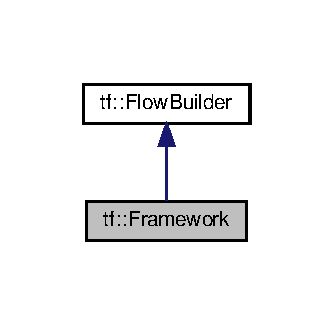
\includegraphics[width=160pt]{classtf_1_1Framework__inherit__graph}
\end{center}
\end{figure}


Collaboration diagram for tf\+:\+:Framework\+:\nopagebreak
\begin{figure}[H]
\begin{center}
\leavevmode
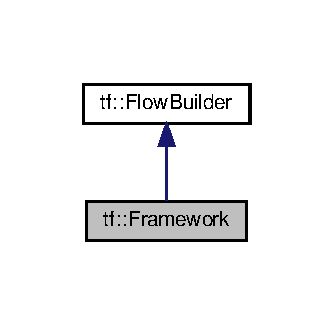
\includegraphics[width=160pt]{classtf_1_1Framework__coll__graph}
\end{center}
\end{figure}
\subsection*{Public Member Functions}
\begin{DoxyCompactItemize}
\item 
\hyperlink{classtf_1_1Framework_a4a9bb59001066e07cbcc9c8f2debb75c}{Framework} ()
\end{DoxyCompactItemize}
\subsection*{Protected Attributes}
\begin{DoxyCompactItemize}
\item 
\hyperlink{namespacetf_a2afa7da139285640eaf8122535136dc9}{Graph} \hyperlink{classtf_1_1Framework_a935110e9ab91f5a520f9354409892d20}{\+\_\+graph}
\end{DoxyCompactItemize}
\subsection*{Friends}
\begin{DoxyCompactItemize}
\item 
{\footnotesize template$<$template$<$ typename... $>$ typename E$>$ }\\class \hyperlink{classtf_1_1Framework_ab3ad8c5c7ed22c3fbd8a41b84db75083}{Basic\+Taskflow}
\end{DoxyCompactItemize}
\subsection*{Additional Inherited Members}


\subsection{Constructor \& Destructor Documentation}
\mbox{\Hypertarget{classtf_1_1Framework_a4a9bb59001066e07cbcc9c8f2debb75c}\label{classtf_1_1Framework_a4a9bb59001066e07cbcc9c8f2debb75c}} 
\index{tf\+::\+Framework@{tf\+::\+Framework}!Framework@{Framework}}
\index{Framework@{Framework}!tf\+::\+Framework@{tf\+::\+Framework}}
\subsubsection{\texorpdfstring{Framework()}{Framework()}}
{\footnotesize\ttfamily tf\+::\+Framework\+::\+Framework (\begin{DoxyParamCaption}{ }\end{DoxyParamCaption})\hspace{0.3cm}{\ttfamily [inline]}}



\subsection{Friends And Related Function Documentation}
\mbox{\Hypertarget{classtf_1_1Framework_ab3ad8c5c7ed22c3fbd8a41b84db75083}\label{classtf_1_1Framework_ab3ad8c5c7ed22c3fbd8a41b84db75083}} 
\index{tf\+::\+Framework@{tf\+::\+Framework}!Basic\+Taskflow@{Basic\+Taskflow}}
\index{Basic\+Taskflow@{Basic\+Taskflow}!tf\+::\+Framework@{tf\+::\+Framework}}
\subsubsection{\texorpdfstring{Basic\+Taskflow}{BasicTaskflow}}
{\footnotesize\ttfamily template$<$template$<$ typename... $>$ typename E$>$ \\
friend class \hyperlink{classtf_1_1BasicTaskflow}{Basic\+Taskflow}\hspace{0.3cm}{\ttfamily [friend]}}



\subsection{Member Data Documentation}
\mbox{\Hypertarget{classtf_1_1Framework_a935110e9ab91f5a520f9354409892d20}\label{classtf_1_1Framework_a935110e9ab91f5a520f9354409892d20}} 
\index{tf\+::\+Framework@{tf\+::\+Framework}!\+\_\+graph@{\+\_\+graph}}
\index{\+\_\+graph@{\+\_\+graph}!tf\+::\+Framework@{tf\+::\+Framework}}
\subsubsection{\texorpdfstring{\+\_\+graph}{\_graph}}
{\footnotesize\ttfamily \hyperlink{namespacetf_a2afa7da139285640eaf8122535136dc9}{Graph} tf\+::\+Framework\+::\+\_\+graph\hspace{0.3cm}{\ttfamily [protected]}}



The documentation for this class was generated from the following file\+:\begin{DoxyCompactItemize}
\item 
/home/twhuang/\+Ph\+D/\+Code/cpp-\/taskflow/taskflow/graph/\hyperlink{framework_8hpp}{framework.\+hpp}\end{DoxyCompactItemize}

\hypertarget{structstd_1_1detail_1_1invoke__impl}{}\section{std\+:\+:detail\+:\+:invoke\+\_\+impl$<$ T $>$ Struct Template Reference}
\label{structstd_1_1detail_1_1invoke__impl}\index{std\+::detail\+::invoke\+\_\+impl$<$ T $>$@{std\+::detail\+::invoke\+\_\+impl$<$ T $>$}}


{\ttfamily \#include $<$threadpool\+\_\+cxx14.\+hpp$>$}

\subsection*{Static Public Member Functions}
\begin{DoxyCompactItemize}
\item 
{\footnotesize template$<$class F , class... Args$>$ }\\static auto \hyperlink{structstd_1_1detail_1_1invoke__impl_abc57075dcca67e9a80242eb4f14611cb}{call} (F \&\&f, Args \&\&... args) -\/$>$ decltype(std\+::forward$<$ F $>$(f)(std\+::forward$<$ Args $>$(args)...))
\end{DoxyCompactItemize}


\subsection{Member Function Documentation}
\mbox{\Hypertarget{structstd_1_1detail_1_1invoke__impl_abc57075dcca67e9a80242eb4f14611cb}\label{structstd_1_1detail_1_1invoke__impl_abc57075dcca67e9a80242eb4f14611cb}} 
\index{std\+::detail\+::invoke\+\_\+impl@{std\+::detail\+::invoke\+\_\+impl}!call@{call}}
\index{call@{call}!std\+::detail\+::invoke\+\_\+impl@{std\+::detail\+::invoke\+\_\+impl}}
\subsubsection{\texorpdfstring{call()}{call()}}
{\footnotesize\ttfamily template$<$class T $>$ \\
template$<$class F , class... Args$>$ \\
static auto \hyperlink{structstd_1_1detail_1_1invoke__impl}{std\+::detail\+::invoke\+\_\+impl}$<$ T $>$\+::call (\begin{DoxyParamCaption}\item[{F \&\&}]{f,  }\item[{Args \&\&...}]{args }\end{DoxyParamCaption}) -\/$>$  decltype(std\+::forward$<$ F $>$(f)(std\+::forward$<$ Args $>$(args)...))\hspace{0.3cm}{\ttfamily [static]}}



The documentation for this struct was generated from the following file\+:\begin{DoxyCompactItemize}
\item 
/home/twhuang/\+Ph\+D/\+Code/cpp-\/taskflow/taskflow/threadpool/\hyperlink{threadpool__cxx14_8hpp}{threadpool\+\_\+cxx14.\+hpp}\end{DoxyCompactItemize}

\hypertarget{structstd_1_1detail_1_1invoke__impl_3_01MT_01B_1_1_5_01_4}{}\section{std\+:\+:detail\+:\+:invoke\+\_\+impl$<$ MT B\+:\+:$\ast$ $>$ Struct Template Reference}
\label{structstd_1_1detail_1_1invoke__impl_3_01MT_01B_1_1_5_01_4}\index{std\+::detail\+::invoke\+\_\+impl$<$ M\+T B\+::$\ast$ $>$@{std\+::detail\+::invoke\+\_\+impl$<$ M\+T B\+::$\ast$ $>$}}


{\ttfamily \#include $<$threadpool\+\_\+cxx14.\+hpp$>$}

\subsection*{Static Public Member Functions}
\begin{DoxyCompactItemize}
\item 
{\footnotesize template$<$class T , class Td  = typename std\+::decay$<$\+T$>$\+::type, class  = typename std\+::enable\+\_\+if$<$std\+::is\+\_\+base\+\_\+of$<$\+B, Td$>$\+::value$>$\+::type$>$ }\\static auto \hyperlink{structstd_1_1detail_1_1invoke__impl_3_01MT_01B_1_1_5_01_4_a5d586e031aeaa0ce27ab99163560fc29}{get} (T \&\&t) -\/$>$ T \&\&
\item 
{\footnotesize template$<$class T , class Td  = typename std\+::decay$<$\+T$>$\+::type, class  = typename std\+::enable\+\_\+if$<$is\+\_\+reference\+\_\+wrapper$<$\+Td$>$\+::value$>$\+::type$>$ }\\static auto \hyperlink{structstd_1_1detail_1_1invoke__impl_3_01MT_01B_1_1_5_01_4_afe48fd9881ae5854f3e78a5186d5a45f}{get} (T \&\&t) -\/$>$ decltype(t.\+get())
\item 
{\footnotesize template$<$class T , class Td  = typename std\+::decay$<$\+T$>$\+::type, class  = typename std\+::enable\+\_\+if$<$!std\+::is\+\_\+base\+\_\+of$<$\+B, Td$>$\+::value$>$\+::type, class  = typename std\+::enable\+\_\+if$<$!is\+\_\+reference\+\_\+wrapper$<$\+Td$>$\+::value$>$\+::type$>$ }\\static auto \hyperlink{structstd_1_1detail_1_1invoke__impl_3_01MT_01B_1_1_5_01_4_af1601009ad460178914b9cec095d8fca}{get} (T \&\&t) -\/$>$ decltype($\ast$std\+::forward$<$ T $>$(t))
\item 
{\footnotesize template$<$class T , class... Args, class M\+T1 , class  = typename std\+::enable\+\_\+if$<$std\+::is\+\_\+function$<$\+M\+T1$>$\+::value$>$\+::type$>$ }\\static auto \hyperlink{structstd_1_1detail_1_1invoke__impl_3_01MT_01B_1_1_5_01_4_aac8b16a210add2424aa7556354b8d815}{call} (M\+T1 B\+::$\ast$pmf, T \&\&t, Args \&\&... args) -\/$>$ decltype((invoke\+\_\+impl\+::get(std\+::forward$<$ T $>$(t)).$\ast$pmf)(std\+::forward$<$ Args $>$(args)...))
\item 
{\footnotesize template$<$class T $>$ }\\static auto \hyperlink{structstd_1_1detail_1_1invoke__impl_3_01MT_01B_1_1_5_01_4_a8c451a7c858ae8dfd8fc34edf8edfe2a}{call} (MT B\+::$\ast$pmd, T \&\&t) -\/$>$ decltype(invoke\+\_\+impl\+::get(std\+::forward$<$ T $>$(t)).$\ast$pmd)
\end{DoxyCompactItemize}


\subsection{Member Function Documentation}
\mbox{\Hypertarget{structstd_1_1detail_1_1invoke__impl_3_01MT_01B_1_1_5_01_4_aac8b16a210add2424aa7556354b8d815}\label{structstd_1_1detail_1_1invoke__impl_3_01MT_01B_1_1_5_01_4_aac8b16a210add2424aa7556354b8d815}} 
\index{std\+::detail\+::invoke\+\_\+impl$<$ M\+T B\+::$\ast$ $>$@{std\+::detail\+::invoke\+\_\+impl$<$ M\+T B\+::$\ast$ $>$}!call@{call}}
\index{call@{call}!std\+::detail\+::invoke\+\_\+impl$<$ M\+T B\+::$\ast$ $>$@{std\+::detail\+::invoke\+\_\+impl$<$ M\+T B\+::$\ast$ $>$}}
\subsubsection{\texorpdfstring{call()}{call()}\hspace{0.1cm}{\footnotesize\ttfamily [1/2]}}
{\footnotesize\ttfamily template$<$class B , class MT $>$ \\
template$<$class T , class... Args, class M\+T1 , class  = typename std\+::enable\+\_\+if$<$std\+::is\+\_\+function$<$\+M\+T1$>$\+::value$>$\+::type$>$ \\
static auto \hyperlink{structstd_1_1detail_1_1invoke__impl}{std\+::detail\+::invoke\+\_\+impl}$<$ MT B\+::$\ast$ $>$\+::call (\begin{DoxyParamCaption}\item[{M\+T1 B\+::$\ast$}]{pmf,  }\item[{T \&\&}]{t,  }\item[{Args \&\&...}]{args }\end{DoxyParamCaption}) -\/$>$  decltype((invoke\+\_\+impl\+::get(std\+::forward$<$ T $>$(t)).$\ast$pmf)(std\+::forward$<$ Args $>$(args)...))\hspace{0.3cm}{\ttfamily [static]}}

\mbox{\Hypertarget{structstd_1_1detail_1_1invoke__impl_3_01MT_01B_1_1_5_01_4_a8c451a7c858ae8dfd8fc34edf8edfe2a}\label{structstd_1_1detail_1_1invoke__impl_3_01MT_01B_1_1_5_01_4_a8c451a7c858ae8dfd8fc34edf8edfe2a}} 
\index{std\+::detail\+::invoke\+\_\+impl$<$ M\+T B\+::$\ast$ $>$@{std\+::detail\+::invoke\+\_\+impl$<$ M\+T B\+::$\ast$ $>$}!call@{call}}
\index{call@{call}!std\+::detail\+::invoke\+\_\+impl$<$ M\+T B\+::$\ast$ $>$@{std\+::detail\+::invoke\+\_\+impl$<$ M\+T B\+::$\ast$ $>$}}
\subsubsection{\texorpdfstring{call()}{call()}\hspace{0.1cm}{\footnotesize\ttfamily [2/2]}}
{\footnotesize\ttfamily template$<$class B , class MT $>$ \\
template$<$class T $>$ \\
static auto \hyperlink{structstd_1_1detail_1_1invoke__impl}{std\+::detail\+::invoke\+\_\+impl}$<$ MT B\+::$\ast$ $>$\+::call (\begin{DoxyParamCaption}\item[{MT B\+::$\ast$}]{pmd,  }\item[{T \&\&}]{t }\end{DoxyParamCaption}) -\/$>$  decltype(invoke\+\_\+impl\+::get(std\+::forward$<$ T $>$(t)).$\ast$pmd)\hspace{0.3cm}{\ttfamily [static]}}

\mbox{\Hypertarget{structstd_1_1detail_1_1invoke__impl_3_01MT_01B_1_1_5_01_4_a5d586e031aeaa0ce27ab99163560fc29}\label{structstd_1_1detail_1_1invoke__impl_3_01MT_01B_1_1_5_01_4_a5d586e031aeaa0ce27ab99163560fc29}} 
\index{std\+::detail\+::invoke\+\_\+impl$<$ M\+T B\+::$\ast$ $>$@{std\+::detail\+::invoke\+\_\+impl$<$ M\+T B\+::$\ast$ $>$}!get@{get}}
\index{get@{get}!std\+::detail\+::invoke\+\_\+impl$<$ M\+T B\+::$\ast$ $>$@{std\+::detail\+::invoke\+\_\+impl$<$ M\+T B\+::$\ast$ $>$}}
\subsubsection{\texorpdfstring{get()}{get()}\hspace{0.1cm}{\footnotesize\ttfamily [1/3]}}
{\footnotesize\ttfamily template$<$class B , class MT $>$ \\
template$<$class T , class Td  = typename std\+::decay$<$\+T$>$\+::type, class  = typename std\+::enable\+\_\+if$<$std\+::is\+\_\+base\+\_\+of$<$\+B, Td$>$\+::value$>$\+::type$>$ \\
static auto \hyperlink{structstd_1_1detail_1_1invoke__impl}{std\+::detail\+::invoke\+\_\+impl}$<$ MT B\+::$\ast$ $>$\+::get (\begin{DoxyParamCaption}\item[{T \&\&}]{t }\end{DoxyParamCaption}) -\/$>$  T \&\&\hspace{0.3cm}{\ttfamily [static]}}

\mbox{\Hypertarget{structstd_1_1detail_1_1invoke__impl_3_01MT_01B_1_1_5_01_4_afe48fd9881ae5854f3e78a5186d5a45f}\label{structstd_1_1detail_1_1invoke__impl_3_01MT_01B_1_1_5_01_4_afe48fd9881ae5854f3e78a5186d5a45f}} 
\index{std\+::detail\+::invoke\+\_\+impl$<$ M\+T B\+::$\ast$ $>$@{std\+::detail\+::invoke\+\_\+impl$<$ M\+T B\+::$\ast$ $>$}!get@{get}}
\index{get@{get}!std\+::detail\+::invoke\+\_\+impl$<$ M\+T B\+::$\ast$ $>$@{std\+::detail\+::invoke\+\_\+impl$<$ M\+T B\+::$\ast$ $>$}}
\subsubsection{\texorpdfstring{get()}{get()}\hspace{0.1cm}{\footnotesize\ttfamily [2/3]}}
{\footnotesize\ttfamily template$<$class B , class MT $>$ \\
template$<$class T , class Td  = typename std\+::decay$<$\+T$>$\+::type, class  = typename std\+::enable\+\_\+if$<$is\+\_\+reference\+\_\+wrapper$<$\+Td$>$\+::value$>$\+::type$>$ \\
static auto \hyperlink{structstd_1_1detail_1_1invoke__impl}{std\+::detail\+::invoke\+\_\+impl}$<$ MT B\+::$\ast$ $>$\+::get (\begin{DoxyParamCaption}\item[{T \&\&}]{t }\end{DoxyParamCaption}) -\/$>$  decltype(t.\+get())\hspace{0.3cm}{\ttfamily [static]}}

\mbox{\Hypertarget{structstd_1_1detail_1_1invoke__impl_3_01MT_01B_1_1_5_01_4_af1601009ad460178914b9cec095d8fca}\label{structstd_1_1detail_1_1invoke__impl_3_01MT_01B_1_1_5_01_4_af1601009ad460178914b9cec095d8fca}} 
\index{std\+::detail\+::invoke\+\_\+impl$<$ M\+T B\+::$\ast$ $>$@{std\+::detail\+::invoke\+\_\+impl$<$ M\+T B\+::$\ast$ $>$}!get@{get}}
\index{get@{get}!std\+::detail\+::invoke\+\_\+impl$<$ M\+T B\+::$\ast$ $>$@{std\+::detail\+::invoke\+\_\+impl$<$ M\+T B\+::$\ast$ $>$}}
\subsubsection{\texorpdfstring{get()}{get()}\hspace{0.1cm}{\footnotesize\ttfamily [3/3]}}
{\footnotesize\ttfamily template$<$class B , class MT $>$ \\
template$<$class T , class Td  = typename std\+::decay$<$\+T$>$\+::type, class  = typename std\+::enable\+\_\+if$<$!std\+::is\+\_\+base\+\_\+of$<$\+B, Td$>$\+::value$>$\+::type, class  = typename std\+::enable\+\_\+if$<$!is\+\_\+reference\+\_\+wrapper$<$\+Td$>$\+::value$>$\+::type$>$ \\
static auto \hyperlink{structstd_1_1detail_1_1invoke__impl}{std\+::detail\+::invoke\+\_\+impl}$<$ MT B\+::$\ast$ $>$\+::get (\begin{DoxyParamCaption}\item[{T \&\&}]{t }\end{DoxyParamCaption}) -\/$>$  decltype($\ast$std\+::forward$<$ T $>$(t))\hspace{0.3cm}{\ttfamily [static]}}



The documentation for this struct was generated from the following file\+:\begin{DoxyCompactItemize}
\item 
/home/twhuang/\+Ph\+D/\+Code/cpp-\/taskflow/taskflow/threadpool/\hyperlink{threadpool__cxx14_8hpp}{threadpool\+\_\+cxx14.\+hpp}\end{DoxyCompactItemize}

\hypertarget{structstd_1_1detail_1_1invoke__result}{}\section{std\+:\+:detail\+:\+:invoke\+\_\+result$<$ Always\+Void, typename,... $>$ Struct Template Reference}
\label{structstd_1_1detail_1_1invoke__result}\index{std\+::detail\+::invoke\+\_\+result$<$ Always\+Void, typename,... $>$@{std\+::detail\+::invoke\+\_\+result$<$ Always\+Void, typename,... $>$}}


{\ttfamily \#include $<$threadpool\+\_\+cxx14.\+hpp$>$}



The documentation for this struct was generated from the following file\+:\begin{DoxyCompactItemize}
\item 
/home/twhuang/\+Ph\+D/\+Code/cpp-\/taskflow/taskflow/threadpool/\hyperlink{threadpool__cxx14_8hpp}{threadpool\+\_\+cxx14.\+hpp}\end{DoxyCompactItemize}

\hypertarget{structstd_1_1invoke__result}{}\section{std\+:\+:invoke\+\_\+result$<$ F, Arg\+Types $>$ Struct Template Reference}
\label{structstd_1_1invoke__result}\index{std\+::invoke\+\_\+result$<$ F, Arg\+Types $>$@{std\+::invoke\+\_\+result$<$ F, Arg\+Types $>$}}


{\ttfamily \#include $<$threadpool\+\_\+cxx14.\+hpp$>$}



Inheritance diagram for std\+:\+:invoke\+\_\+result$<$ F, Arg\+Types $>$\+:\nopagebreak
\begin{figure}[H]
\begin{center}
\leavevmode
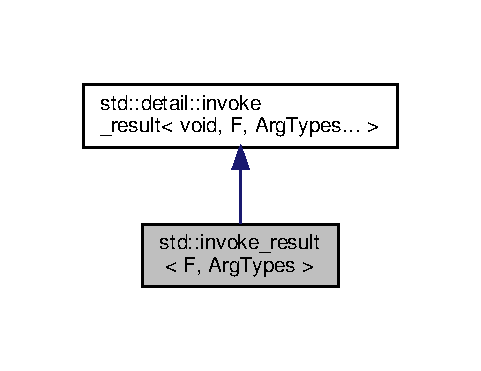
\includegraphics[width=231pt]{structstd_1_1invoke__result__inherit__graph}
\end{center}
\end{figure}


Collaboration diagram for std\+:\+:invoke\+\_\+result$<$ F, Arg\+Types $>$\+:\nopagebreak
\begin{figure}[H]
\begin{center}
\leavevmode
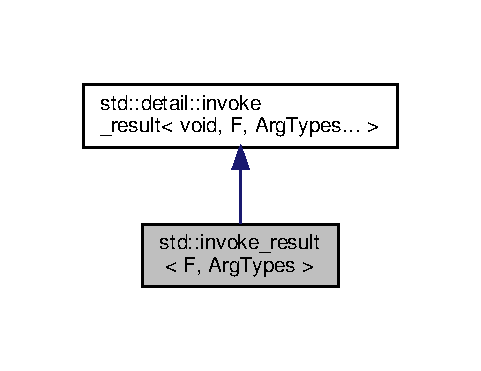
\includegraphics[width=231pt]{structstd_1_1invoke__result__coll__graph}
\end{center}
\end{figure}


The documentation for this struct was generated from the following file\+:\begin{DoxyCompactItemize}
\item 
/home/twhuang/\+Ph\+D/\+Code/cpp-\/taskflow/taskflow/threadpool/\hyperlink{threadpool__cxx14_8hpp}{threadpool\+\_\+cxx14.\+hpp}\end{DoxyCompactItemize}

\hypertarget{structstd_1_1detail_1_1invoke__result_3_01decltype_07void_07detail_1_1INVOKE_07std_1_1declval_3_86a9900dcd4a84f000244f479e0f71a8}{}\section{std\+:\+:detail\+:\+:invoke\+\_\+result$<$ decltype(void(detail\+:\+:I\+N\+V\+O\+KE(std\+:\+:declval$<$ F $>$(), std\+:\+:declval$<$ Args $>$()...))), F, Args... $>$ Struct Template Reference}
\label{structstd_1_1detail_1_1invoke__result_3_01decltype_07void_07detail_1_1INVOKE_07std_1_1declval_3_86a9900dcd4a84f000244f479e0f71a8}\index{std\+::detail\+::invoke\+\_\+result$<$ decltype(void(detail\+::\+I\+N\+V\+O\+K\+E(std\+::declval$<$ F $>$(), std\+::declval$<$ Args $>$()...))), F, Args... $>$@{std\+::detail\+::invoke\+\_\+result$<$ decltype(void(detail\+::\+I\+N\+V\+O\+K\+E(std\+::declval$<$ F $>$(), std\+::declval$<$ Args $>$()...))), F, Args... $>$}}


{\ttfamily \#include $<$threadpool\+\_\+cxx14.\+hpp$>$}

\subsection*{Public Types}
\begin{DoxyCompactItemize}
\item 
using \hyperlink{structstd_1_1detail_1_1invoke__result_3_01decltype_07void_07detail_1_1INVOKE_07std_1_1declval_3_86a9900dcd4a84f000244f479e0f71a8_a23231eda2a8247ba660dd6c3146fe3ed}{type} = decltype(\hyperlink{namespacestd_1_1detail_ac5263dda7d727dde5281b6b1da8ebb79}{detail\+::\+I\+N\+V\+O\+KE}(std\+::declval$<$ F $>$(), std\+::declval$<$ Args $>$()...))
\end{DoxyCompactItemize}


\subsection{Member Typedef Documentation}
\mbox{\Hypertarget{structstd_1_1detail_1_1invoke__result_3_01decltype_07void_07detail_1_1INVOKE_07std_1_1declval_3_86a9900dcd4a84f000244f479e0f71a8_a23231eda2a8247ba660dd6c3146fe3ed}\label{structstd_1_1detail_1_1invoke__result_3_01decltype_07void_07detail_1_1INVOKE_07std_1_1declval_3_86a9900dcd4a84f000244f479e0f71a8_a23231eda2a8247ba660dd6c3146fe3ed}} 
\index{std\+::detail\+::invoke\+\_\+result$<$ decltype(void(detail\+::\+I\+N\+V\+O\+K\+E(std\+::declval$<$ F $>$(), std\+::declval$<$ Args $>$()...))), F, Args... $>$@{std\+::detail\+::invoke\+\_\+result$<$ decltype(void(detail\+::\+I\+N\+V\+O\+K\+E(std\+::declval$<$ F $>$(), std\+::declval$<$ Args $>$()...))), F, Args... $>$}!type@{type}}
\index{type@{type}!std\+::detail\+::invoke\+\_\+result$<$ decltype(void(detail\+::\+I\+N\+V\+O\+K\+E(std\+::declval$<$ F $>$(), std\+::declval$<$ Args $>$()...))), F, Args... $>$@{std\+::detail\+::invoke\+\_\+result$<$ decltype(void(detail\+::\+I\+N\+V\+O\+K\+E(std\+::declval$<$ F $>$(), std\+::declval$<$ Args $>$()...))), F, Args... $>$}}
\subsubsection{\texorpdfstring{type}{type}}
{\footnotesize\ttfamily template$<$typename F , typename... Args$>$ \\
using \hyperlink{structstd_1_1detail_1_1invoke__result}{std\+::detail\+::invoke\+\_\+result}$<$ decltype(void(\hyperlink{namespacestd_1_1detail_ac5263dda7d727dde5281b6b1da8ebb79}{detail\+::\+I\+N\+V\+O\+KE}(std\+::declval$<$ F $>$(), std\+::declval$<$ Args $>$()...))), F, Args... $>$\+::\hyperlink{structstd_1_1detail_1_1invoke__result_3_01decltype_07void_07detail_1_1INVOKE_07std_1_1declval_3_86a9900dcd4a84f000244f479e0f71a8_a23231eda2a8247ba660dd6c3146fe3ed}{type} =  decltype(\hyperlink{namespacestd_1_1detail_ac5263dda7d727dde5281b6b1da8ebb79}{detail\+::\+I\+N\+V\+O\+KE}(std\+::declval$<$F$>$(), std\+::declval$<$Args$>$()...))}



The documentation for this struct was generated from the following file\+:\begin{DoxyCompactItemize}
\item 
/home/twhuang/\+Ph\+D/\+Code/cpp-\/taskflow/taskflow/threadpool/\hyperlink{threadpool__cxx14_8hpp}{threadpool\+\_\+cxx14.\+hpp}\end{DoxyCompactItemize}

\hypertarget{structstd_1_1is__error__code__enum_3_01tf_1_1Error_1_1Code_01_4}{}\section{std\+:\+:is\+\_\+error\+\_\+code\+\_\+enum$<$ tf\+:\+:Error\+:\+:Code $>$ Struct Template Reference}
\label{structstd_1_1is__error__code__enum_3_01tf_1_1Error_1_1Code_01_4}\index{std\+::is\+\_\+error\+\_\+code\+\_\+enum$<$ tf\+::\+Error\+::\+Code $>$@{std\+::is\+\_\+error\+\_\+code\+\_\+enum$<$ tf\+::\+Error\+::\+Code $>$}}


{\ttfamily \#include $<$error.\+hpp$>$}



Inheritance diagram for std\+:\+:is\+\_\+error\+\_\+code\+\_\+enum$<$ tf\+:\+:Error\+:\+:Code $>$\+:\nopagebreak
\begin{figure}[H]
\begin{center}
\leavevmode
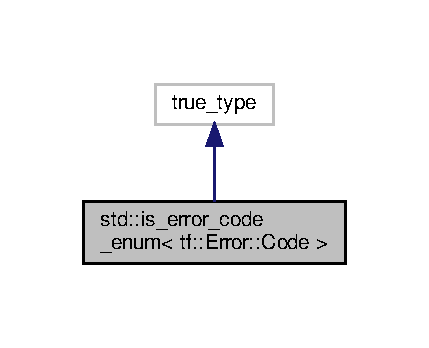
\includegraphics[width=206pt]{structstd_1_1is__error__code__enum_3_01tf_1_1Error_1_1Code_01_4__inherit__graph}
\end{center}
\end{figure}


Collaboration diagram for std\+:\+:is\+\_\+error\+\_\+code\+\_\+enum$<$ tf\+:\+:Error\+:\+:Code $>$\+:\nopagebreak
\begin{figure}[H]
\begin{center}
\leavevmode
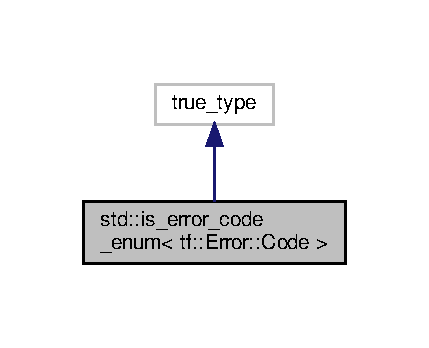
\includegraphics[width=206pt]{structstd_1_1is__error__code__enum_3_01tf_1_1Error_1_1Code_01_4__coll__graph}
\end{center}
\end{figure}


The documentation for this struct was generated from the following file\+:\begin{DoxyCompactItemize}
\item 
/home/twhuang/\+Ph\+D/\+Code/cpp-\/taskflow/taskflow/error/\hyperlink{error_8hpp}{error.\+hpp}\end{DoxyCompactItemize}

\hypertarget{structtf_1_1is__iterable}{}\section{tf\+:\+:is\+\_\+iterable$<$ T, typename $>$ Struct Template Reference}
\label{structtf_1_1is__iterable}\index{tf\+::is\+\_\+iterable$<$ T, typename $>$@{tf\+::is\+\_\+iterable$<$ T, typename $>$}}


{\ttfamily \#include $<$utility.\+hpp$>$}



Inheritance diagram for tf\+:\+:is\+\_\+iterable$<$ T, typename $>$\+:\nopagebreak
\begin{figure}[H]
\begin{center}
\leavevmode
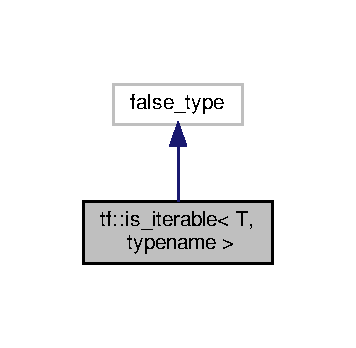
\includegraphics[width=171pt]{structtf_1_1is__iterable__inherit__graph}
\end{center}
\end{figure}


Collaboration diagram for tf\+:\+:is\+\_\+iterable$<$ T, typename $>$\+:\nopagebreak
\begin{figure}[H]
\begin{center}
\leavevmode
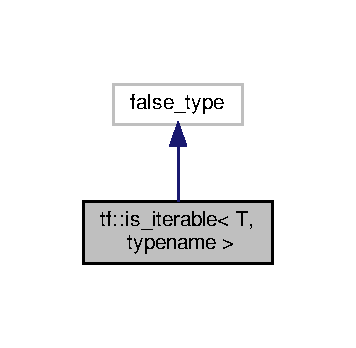
\includegraphics[width=171pt]{structtf_1_1is__iterable__coll__graph}
\end{center}
\end{figure}


The documentation for this struct was generated from the following file\+:\begin{DoxyCompactItemize}
\item 
/home/twhuang/\+Ph\+D/\+Code/cpp-\/taskflow/taskflow/utility/\hyperlink{utility_8hpp}{utility.\+hpp}\end{DoxyCompactItemize}

\hypertarget{structtf_1_1is__iterable_3_01T_00_01std_1_1void__t_3_01decltype_07std_1_1declval_3_01T_01_4_07_0275ba78d7ba399cf74de163921d814a0}{}\section{tf\+:\+:is\+\_\+iterable$<$ T, std\+:\+:void\+\_\+t$<$ decltype(std\+:\+:declval$<$ T $>$().begin()), decltype(std\+:\+:declval$<$ T $>$().end())$>$ $>$ Struct Template Reference}
\label{structtf_1_1is__iterable_3_01T_00_01std_1_1void__t_3_01decltype_07std_1_1declval_3_01T_01_4_07_0275ba78d7ba399cf74de163921d814a0}\index{tf\+::is\+\_\+iterable$<$ T, std\+::void\+\_\+t$<$ decltype(std\+::declval$<$ T $>$().\+begin()), decltype(std\+::declval$<$ T $>$().\+end())$>$ $>$@{tf\+::is\+\_\+iterable$<$ T, std\+::void\+\_\+t$<$ decltype(std\+::declval$<$ T $>$().\+begin()), decltype(std\+::declval$<$ T $>$().\+end())$>$ $>$}}


{\ttfamily \#include $<$utility.\+hpp$>$}



Inheritance diagram for tf\+:\+:is\+\_\+iterable$<$ T, std\+:\+:void\+\_\+t$<$ decltype(std\+:\+:declval$<$ T $>$().begin()), decltype(std\+:\+:declval$<$ T $>$().end())$>$ $>$\+:\nopagebreak
\begin{figure}[H]
\begin{center}
\leavevmode
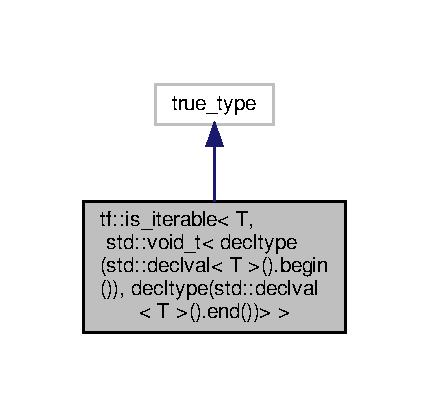
\includegraphics[width=206pt]{structtf_1_1is__iterable_3_01T_00_01std_1_1void__t_3_01decltype_07std_1_1declval_3_01T_01_4_07_09bc73e59e9f10718f4eac50bdd178d5a}
\end{center}
\end{figure}


Collaboration diagram for tf\+:\+:is\+\_\+iterable$<$ T, std\+:\+:void\+\_\+t$<$ decltype(std\+:\+:declval$<$ T $>$().begin()), decltype(std\+:\+:declval$<$ T $>$().end())$>$ $>$\+:\nopagebreak
\begin{figure}[H]
\begin{center}
\leavevmode
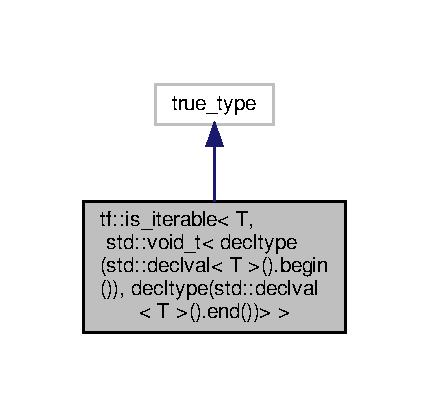
\includegraphics[width=206pt]{structtf_1_1is__iterable_3_01T_00_01std_1_1void__t_3_01decltype_07std_1_1declval_3_01T_01_4_07_09bc35699403c124a31814ace50d8a718}
\end{center}
\end{figure}


The documentation for this struct was generated from the following file\+:\begin{DoxyCompactItemize}
\item 
/home/twhuang/\+Ph\+D/\+Code/cpp-\/taskflow/taskflow/utility/\hyperlink{utility_8hpp}{utility.\+hpp}\end{DoxyCompactItemize}

\hypertarget{structtf_1_1is__iterator}{}\section{tf\+:\+:is\+\_\+iterator$<$ T, typename $>$ Struct Template Reference}
\label{structtf_1_1is__iterator}\index{tf\+::is\+\_\+iterator$<$ T, typename $>$@{tf\+::is\+\_\+iterator$<$ T, typename $>$}}


{\ttfamily \#include $<$utility.\+hpp$>$}

\subsection*{Static Public Attributes}
\begin{DoxyCompactItemize}
\item 
static constexpr bool \hyperlink{structtf_1_1is__iterator_a5ba3fa7030b45a59913b999a8c1b8419}{value} = false
\end{DoxyCompactItemize}


\subsection{Member Data Documentation}
\mbox{\Hypertarget{structtf_1_1is__iterator_a5ba3fa7030b45a59913b999a8c1b8419}\label{structtf_1_1is__iterator_a5ba3fa7030b45a59913b999a8c1b8419}} 
\index{tf\+::is\+\_\+iterator@{tf\+::is\+\_\+iterator}!value@{value}}
\index{value@{value}!tf\+::is\+\_\+iterator@{tf\+::is\+\_\+iterator}}
\subsubsection{\texorpdfstring{value}{value}}
{\footnotesize\ttfamily template$<$typename T , typename  = void$>$ \\
constexpr bool \hyperlink{structtf_1_1is__iterator}{tf\+::is\+\_\+iterator}$<$ T, typename $>$\+::value = false\hspace{0.3cm}{\ttfamily [static]}}



The documentation for this struct was generated from the following file\+:\begin{DoxyCompactItemize}
\item 
/home/twhuang/\+Ph\+D/\+Code/cpp-\/taskflow/taskflow/utility/\hyperlink{utility_8hpp}{utility.\+hpp}\end{DoxyCompactItemize}

\hypertarget{structstd_1_1detail_1_1is__reference__wrapper}{}\section{std\+:\+:detail\+:\+:is\+\_\+reference\+\_\+wrapper$<$ T $>$ Struct Template Reference}
\label{structstd_1_1detail_1_1is__reference__wrapper}\index{std\+::detail\+::is\+\_\+reference\+\_\+wrapper$<$ T $>$@{std\+::detail\+::is\+\_\+reference\+\_\+wrapper$<$ T $>$}}


{\ttfamily \#include $<$threadpool\+\_\+cxx14.\+hpp$>$}



Inheritance diagram for std\+:\+:detail\+:\+:is\+\_\+reference\+\_\+wrapper$<$ T $>$\+:\nopagebreak
\begin{figure}[H]
\begin{center}
\leavevmode
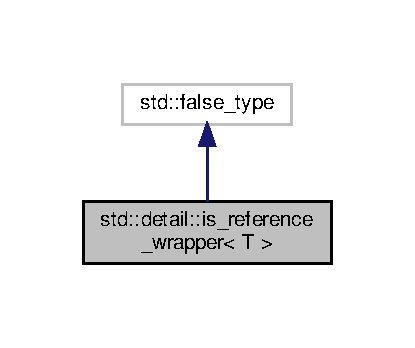
\includegraphics[width=199pt]{structstd_1_1detail_1_1is__reference__wrapper__inherit__graph}
\end{center}
\end{figure}


Collaboration diagram for std\+:\+:detail\+:\+:is\+\_\+reference\+\_\+wrapper$<$ T $>$\+:\nopagebreak
\begin{figure}[H]
\begin{center}
\leavevmode
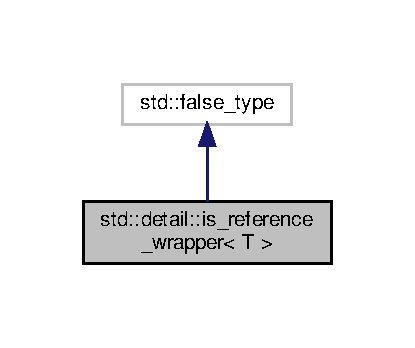
\includegraphics[width=199pt]{structstd_1_1detail_1_1is__reference__wrapper__coll__graph}
\end{center}
\end{figure}


The documentation for this struct was generated from the following file\+:\begin{DoxyCompactItemize}
\item 
/home/twhuang/\+Ph\+D/\+Code/cpp-\/taskflow/taskflow/threadpool/\hyperlink{threadpool__cxx14_8hpp}{threadpool\+\_\+cxx14.\+hpp}\end{DoxyCompactItemize}

\hypertarget{structstd_1_1detail_1_1is__reference__wrapper_3_01std_1_1reference__wrapper_3_01U_01_4_01_4}{}\section{std\+:\+:detail\+:\+:is\+\_\+reference\+\_\+wrapper$<$ std\+:\+:reference\+\_\+wrapper$<$ U $>$ $>$ Struct Template Reference}
\label{structstd_1_1detail_1_1is__reference__wrapper_3_01std_1_1reference__wrapper_3_01U_01_4_01_4}\index{std\+::detail\+::is\+\_\+reference\+\_\+wrapper$<$ std\+::reference\+\_\+wrapper$<$ U $>$ $>$@{std\+::detail\+::is\+\_\+reference\+\_\+wrapper$<$ std\+::reference\+\_\+wrapper$<$ U $>$ $>$}}


{\ttfamily \#include $<$threadpool\+\_\+cxx14.\+hpp$>$}



Inheritance diagram for std\+:\+:detail\+:\+:is\+\_\+reference\+\_\+wrapper$<$ std\+:\+:reference\+\_\+wrapper$<$ U $>$ $>$\+:\nopagebreak
\begin{figure}[H]
\begin{center}
\leavevmode
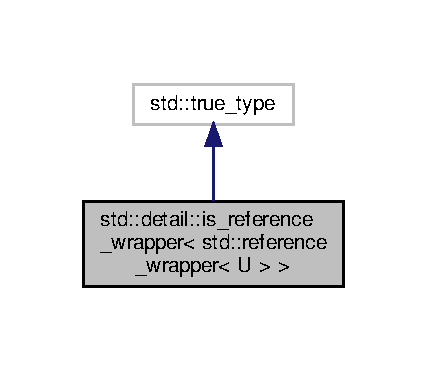
\includegraphics[width=205pt]{structstd_1_1detail_1_1is__reference__wrapper_3_01std_1_1reference__wrapper_3_01U_01_4_01_4__inherit__graph}
\end{center}
\end{figure}


Collaboration diagram for std\+:\+:detail\+:\+:is\+\_\+reference\+\_\+wrapper$<$ std\+:\+:reference\+\_\+wrapper$<$ U $>$ $>$\+:\nopagebreak
\begin{figure}[H]
\begin{center}
\leavevmode
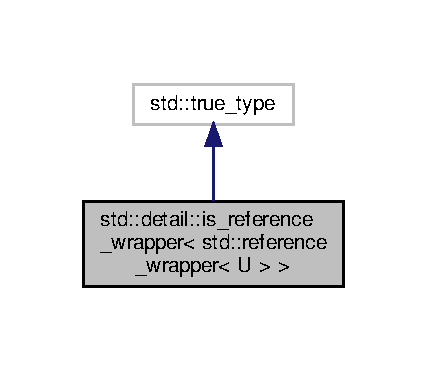
\includegraphics[width=205pt]{structstd_1_1detail_1_1is__reference__wrapper_3_01std_1_1reference__wrapper_3_01U_01_4_01_4__coll__graph}
\end{center}
\end{figure}


The documentation for this struct was generated from the following file\+:\begin{DoxyCompactItemize}
\item 
/home/twhuang/\+Ph\+D/\+Code/cpp-\/taskflow/taskflow/threadpool/\hyperlink{threadpool__cxx14_8hpp}{threadpool\+\_\+cxx14.\+hpp}\end{DoxyCompactItemize}

\hypertarget{structtf_1_1is__iterator_3_01T_00_01std_1_1enable__if__t_3_9std_1_1is__same__v_3_01typename_01st0a3680c192bddd4961327b11d4422a82}{}\section{tf\+:\+:is\+\_\+same\+\_\+v$<$ typename std\+:\+:iterator\+\_\+traits$<$ T $>$\+:\+:value\+\_\+type, void $>$ $>$$>$ Struct Template Reference}
\label{structtf_1_1is__iterator_3_01T_00_01std_1_1enable__if__t_3_9std_1_1is__same__v_3_01typename_01st0a3680c192bddd4961327b11d4422a82}\index{tf\+::is\+\_\+same\+\_\+v$<$ typename std\+::iterator\+\_\+traits$<$ T $>$\+::value\+\_\+type, void $>$ $>$$>$@{tf\+::is\+\_\+same\+\_\+v$<$ typename std\+::iterator\+\_\+traits$<$ T $>$\+::value\+\_\+type, void $>$ $>$$>$}}


{\ttfamily \#include $<$utility.\+hpp$>$}

\subsection*{Static Public Attributes}
\begin{DoxyCompactItemize}
\item 
static constexpr bool \hyperlink{structtf_1_1is__iterator_3_01T_00_01std_1_1enable__if__t_3_9std_1_1is__same__v_3_01typename_01st0a3680c192bddd4961327b11d4422a82_aaa868e82495ecf97fae1bad2dcd94887}{value} = true
\end{DoxyCompactItemize}


\subsection{Member Data Documentation}
\mbox{\Hypertarget{structtf_1_1is__iterator_3_01T_00_01std_1_1enable__if__t_3_9std_1_1is__same__v_3_01typename_01st0a3680c192bddd4961327b11d4422a82_aaa868e82495ecf97fae1bad2dcd94887}\label{structtf_1_1is__iterator_3_01T_00_01std_1_1enable__if__t_3_9std_1_1is__same__v_3_01typename_01st0a3680c192bddd4961327b11d4422a82_aaa868e82495ecf97fae1bad2dcd94887}} 
\index{tf\+::is\+\_\+iterator$<$ T, std\+::enable\+\_\+if\+\_\+t$<$"!std\+::is\+\_\+same\+\_\+v$<$ typename std\+::iterator\+\_\+traits$<$ T $>$\+::value\+\_\+type, void $>$ $>$$>$@{tf\+::is\+\_\+iterator$<$ T, std\+::enable\+\_\+if\+\_\+t$<$"!std\+::is\+\_\+same\+\_\+v$<$ typename std\+::iterator\+\_\+traits$<$ T $>$\+::value\+\_\+type, void $>$ $>$$>$}!value@{value}}
\index{value@{value}!tf\+::is\+\_\+iterator$<$ T, std\+::enable\+\_\+if\+\_\+t$<$"!std\+::is\+\_\+same\+\_\+v$<$ typename std\+::iterator\+\_\+traits$<$ T $>$\+::value\+\_\+type, void $>$ $>$$>$@{tf\+::is\+\_\+iterator$<$ T, std\+::enable\+\_\+if\+\_\+t$<$"!std\+::is\+\_\+same\+\_\+v$<$ typename std\+::iterator\+\_\+traits$<$ T $>$\+::value\+\_\+type, void $>$ $>$$>$}}
\subsubsection{\texorpdfstring{value}{value}}
{\footnotesize\ttfamily template$<$typename T $>$ \\
constexpr bool tf\+::is\+\_\+same\+\_\+v$<$ typename std\+::iterator\+\_\+traits$<$ T $>$\+::value\+\_\+type, void $>$ $>$$>$\+::value = true\hspace{0.3cm}{\ttfamily [static]}}



The documentation for this struct was generated from the following file\+:\begin{DoxyCompactItemize}
\item 
/home/twhuang/\+Ph\+D/\+Code/cpp-\/taskflow/taskflow/utility/\hyperlink{utility_8hpp}{utility.\+hpp}\end{DoxyCompactItemize}

\hypertarget{structtf_1_1MoC}{}\section{tf\+:\+:MoC$<$ T $>$ Struct Template Reference}
\label{structtf_1_1MoC}\index{tf\+::\+Mo\+C$<$ T $>$@{tf\+::\+Mo\+C$<$ T $>$}}


{\ttfamily \#include $<$threadpool\+\_\+cxx14.\+hpp$>$}

\subsection*{Public Member Functions}
\begin{DoxyCompactItemize}
\item 
\hyperlink{structtf_1_1MoC_a38c6a89465e651e5e0e9001a9abc42b5}{MoC} (T \&\&rhs)
\item 
\hyperlink{structtf_1_1MoC_a779c86ab4750cd65cdb467065daa70f3}{MoC} (const \hyperlink{structtf_1_1MoC}{MoC} \&other)
\item 
T \& \hyperlink{structtf_1_1MoC_ab6291eb8f0d85484203bb79456ae9816}{get} ()
\item 
\hyperlink{structtf_1_1MoC_a38c6a89465e651e5e0e9001a9abc42b5}{MoC} (T \&\&rhs)
\item 
\hyperlink{structtf_1_1MoC_a779c86ab4750cd65cdb467065daa70f3}{MoC} (const \hyperlink{structtf_1_1MoC}{MoC} \&other)
\item 
T \& \hyperlink{structtf_1_1MoC_ab6291eb8f0d85484203bb79456ae9816}{get} ()
\end{DoxyCompactItemize}
\subsection*{Public Attributes}
\begin{DoxyCompactItemize}
\item 
T \hyperlink{structtf_1_1MoC_a6638e1dc2bd032df12bb48584eabe71e}{object}
\end{DoxyCompactItemize}


\subsection{Constructor \& Destructor Documentation}
\mbox{\Hypertarget{structtf_1_1MoC_a38c6a89465e651e5e0e9001a9abc42b5}\label{structtf_1_1MoC_a38c6a89465e651e5e0e9001a9abc42b5}} 
\index{tf\+::\+MoC@{tf\+::\+MoC}!MoC@{MoC}}
\index{MoC@{MoC}!tf\+::\+MoC@{tf\+::\+MoC}}
\subsubsection{\texorpdfstring{Mo\+C()}{MoC()}\hspace{0.1cm}{\footnotesize\ttfamily [1/4]}}
{\footnotesize\ttfamily template$<$typename T $>$ \\
\hyperlink{structtf_1_1MoC}{tf\+::\+MoC}$<$ T $>$\+::\hyperlink{structtf_1_1MoC}{MoC} (\begin{DoxyParamCaption}\item[{T \&\&}]{rhs }\end{DoxyParamCaption})\hspace{0.3cm}{\ttfamily [inline]}}

\mbox{\Hypertarget{structtf_1_1MoC_a779c86ab4750cd65cdb467065daa70f3}\label{structtf_1_1MoC_a779c86ab4750cd65cdb467065daa70f3}} 
\index{tf\+::\+MoC@{tf\+::\+MoC}!MoC@{MoC}}
\index{MoC@{MoC}!tf\+::\+MoC@{tf\+::\+MoC}}
\subsubsection{\texorpdfstring{Mo\+C()}{MoC()}\hspace{0.1cm}{\footnotesize\ttfamily [2/4]}}
{\footnotesize\ttfamily template$<$typename T $>$ \\
\hyperlink{structtf_1_1MoC}{tf\+::\+MoC}$<$ T $>$\+::\hyperlink{structtf_1_1MoC}{MoC} (\begin{DoxyParamCaption}\item[{const \hyperlink{structtf_1_1MoC}{MoC}$<$ T $>$ \&}]{other }\end{DoxyParamCaption})\hspace{0.3cm}{\ttfamily [inline]}}

\mbox{\Hypertarget{structtf_1_1MoC_a38c6a89465e651e5e0e9001a9abc42b5}\label{structtf_1_1MoC_a38c6a89465e651e5e0e9001a9abc42b5}} 
\index{tf\+::\+MoC@{tf\+::\+MoC}!MoC@{MoC}}
\index{MoC@{MoC}!tf\+::\+MoC@{tf\+::\+MoC}}
\subsubsection{\texorpdfstring{Mo\+C()}{MoC()}\hspace{0.1cm}{\footnotesize\ttfamily [3/4]}}
{\footnotesize\ttfamily template$<$typename T $>$ \\
\hyperlink{structtf_1_1MoC}{tf\+::\+MoC}$<$ T $>$\+::\hyperlink{structtf_1_1MoC}{MoC} (\begin{DoxyParamCaption}\item[{T \&\&}]{rhs }\end{DoxyParamCaption})\hspace{0.3cm}{\ttfamily [inline]}}

\mbox{\Hypertarget{structtf_1_1MoC_a779c86ab4750cd65cdb467065daa70f3}\label{structtf_1_1MoC_a779c86ab4750cd65cdb467065daa70f3}} 
\index{tf\+::\+MoC@{tf\+::\+MoC}!MoC@{MoC}}
\index{MoC@{MoC}!tf\+::\+MoC@{tf\+::\+MoC}}
\subsubsection{\texorpdfstring{Mo\+C()}{MoC()}\hspace{0.1cm}{\footnotesize\ttfamily [4/4]}}
{\footnotesize\ttfamily template$<$typename T $>$ \\
\hyperlink{structtf_1_1MoC}{tf\+::\+MoC}$<$ T $>$\+::\hyperlink{structtf_1_1MoC}{MoC} (\begin{DoxyParamCaption}\item[{const \hyperlink{structtf_1_1MoC}{MoC}$<$ T $>$ \&}]{other }\end{DoxyParamCaption})\hspace{0.3cm}{\ttfamily [inline]}}



\subsection{Member Function Documentation}
\mbox{\Hypertarget{structtf_1_1MoC_ab6291eb8f0d85484203bb79456ae9816}\label{structtf_1_1MoC_ab6291eb8f0d85484203bb79456ae9816}} 
\index{tf\+::\+MoC@{tf\+::\+MoC}!get@{get}}
\index{get@{get}!tf\+::\+MoC@{tf\+::\+MoC}}
\subsubsection{\texorpdfstring{get()}{get()}\hspace{0.1cm}{\footnotesize\ttfamily [1/2]}}
{\footnotesize\ttfamily template$<$typename T $>$ \\
T\& \hyperlink{structtf_1_1MoC}{tf\+::\+MoC}$<$ T $>$\+::get (\begin{DoxyParamCaption}{ }\end{DoxyParamCaption})\hspace{0.3cm}{\ttfamily [inline]}}

\mbox{\Hypertarget{structtf_1_1MoC_ab6291eb8f0d85484203bb79456ae9816}\label{structtf_1_1MoC_ab6291eb8f0d85484203bb79456ae9816}} 
\index{tf\+::\+MoC@{tf\+::\+MoC}!get@{get}}
\index{get@{get}!tf\+::\+MoC@{tf\+::\+MoC}}
\subsubsection{\texorpdfstring{get()}{get()}\hspace{0.1cm}{\footnotesize\ttfamily [2/2]}}
{\footnotesize\ttfamily template$<$typename T $>$ \\
T\& \hyperlink{structtf_1_1MoC}{tf\+::\+MoC}$<$ T $>$\+::get (\begin{DoxyParamCaption}{ }\end{DoxyParamCaption})\hspace{0.3cm}{\ttfamily [inline]}}



\subsection{Member Data Documentation}
\mbox{\Hypertarget{structtf_1_1MoC_a6638e1dc2bd032df12bb48584eabe71e}\label{structtf_1_1MoC_a6638e1dc2bd032df12bb48584eabe71e}} 
\index{tf\+::\+MoC@{tf\+::\+MoC}!object@{object}}
\index{object@{object}!tf\+::\+MoC@{tf\+::\+MoC}}
\subsubsection{\texorpdfstring{object}{object}}
{\footnotesize\ttfamily template$<$typename T $>$ \\
T \hyperlink{structtf_1_1MoC}{tf\+::\+MoC}$<$ T $>$\+::object\hspace{0.3cm}{\ttfamily [mutable]}}



The documentation for this struct was generated from the following files\+:\begin{DoxyCompactItemize}
\item 
/home/twhuang/\+Ph\+D/\+Code/cpp-\/taskflow/taskflow/threadpool/\hyperlink{threadpool__cxx14_8hpp}{threadpool\+\_\+cxx14.\+hpp}\item 
/home/twhuang/\+Ph\+D/\+Code/cpp-\/taskflow/taskflow/utility/\hyperlink{utility_8hpp}{utility.\+hpp}\end{DoxyCompactItemize}

\hypertarget{classtf_1_1Node}{}\section{tf\+:\+:Node Class Reference}
\label{classtf_1_1Node}\index{tf\+::\+Node@{tf\+::\+Node}}


{\ttfamily \#include $<$graph.\+hpp$>$}

\subsection*{Public Member Functions}
\begin{DoxyCompactItemize}
\item 
\hyperlink{classtf_1_1Node_a6b1092cf320099a755253a6272d71e66}{Node} ()
\item 
{\footnotesize template$<$typename C $>$ }\\\hyperlink{classtf_1_1Node_ac4f83d80151907262972711fdfdcb177}{Node} (C \&\&)
\item 
const std\+::string \& \hyperlink{classtf_1_1Node_a0214bc98366d4c24a1cae941cdffe119}{name} () const
\item 
void \hyperlink{classtf_1_1Node_a753839c8159372098e7f48158229865c}{precede} (\hyperlink{classtf_1_1Node}{Node} \&)
\item 
void \hyperlink{classtf_1_1Node_a5b52f4d47173b28917d7361ea8af06d3}{dump} (std\+::ostream \&) const
\item 
size\+\_\+t \hyperlink{classtf_1_1Node_a7133911e093d82e5f5edd73124b60c6a}{num\+\_\+successors} () const
\item 
size\+\_\+t \hyperlink{classtf_1_1Node_abbb6a85cc8f62682ce8c78ad9851c0e5}{num\+\_\+dependents} () const
\item 
std\+::string \hyperlink{classtf_1_1Node_a0e398a8d70354ff11619bf5e603cbeb7}{dump} () const
\end{DoxyCompactItemize}
\subsection*{Friends}
\begin{DoxyCompactItemize}
\item 
class \hyperlink{classtf_1_1Node_aaa7728226b6ce66782e8816b1658dd9a}{Task}
\item 
class \hyperlink{classtf_1_1Node_acd2b8699ab7559c0da687cd775e2c778}{Topology}
\item 
{\footnotesize template$<$template$<$ typename... $>$ typename E$>$ }\\class \hyperlink{classtf_1_1Node_ab3ad8c5c7ed22c3fbd8a41b84db75083}{Basic\+Taskflow}
\end{DoxyCompactItemize}


\subsection{Constructor \& Destructor Documentation}
\mbox{\Hypertarget{classtf_1_1Node_a6b1092cf320099a755253a6272d71e66}\label{classtf_1_1Node_a6b1092cf320099a755253a6272d71e66}} 
\index{tf\+::\+Node@{tf\+::\+Node}!Node@{Node}}
\index{Node@{Node}!tf\+::\+Node@{tf\+::\+Node}}
\subsubsection{\texorpdfstring{Node()}{Node()}\hspace{0.1cm}{\footnotesize\ttfamily [1/2]}}
{\footnotesize\ttfamily tf\+::\+Node\+::\+Node (\begin{DoxyParamCaption}{ }\end{DoxyParamCaption})\hspace{0.3cm}{\ttfamily [inline]}}

\mbox{\Hypertarget{classtf_1_1Node_ac4f83d80151907262972711fdfdcb177}\label{classtf_1_1Node_ac4f83d80151907262972711fdfdcb177}} 
\index{tf\+::\+Node@{tf\+::\+Node}!Node@{Node}}
\index{Node@{Node}!tf\+::\+Node@{tf\+::\+Node}}
\subsubsection{\texorpdfstring{Node()}{Node()}\hspace{0.1cm}{\footnotesize\ttfamily [2/2]}}
{\footnotesize\ttfamily template$<$typename C $>$ \\
tf\+::\+Node\+::\+Node (\begin{DoxyParamCaption}\item[{C \&\&}]{c }\end{DoxyParamCaption})\hspace{0.3cm}{\ttfamily [inline]}}



\subsection{Member Function Documentation}
\mbox{\Hypertarget{classtf_1_1Node_a5b52f4d47173b28917d7361ea8af06d3}\label{classtf_1_1Node_a5b52f4d47173b28917d7361ea8af06d3}} 
\index{tf\+::\+Node@{tf\+::\+Node}!dump@{dump}}
\index{dump@{dump}!tf\+::\+Node@{tf\+::\+Node}}
\subsubsection{\texorpdfstring{dump()}{dump()}\hspace{0.1cm}{\footnotesize\ttfamily [1/2]}}
{\footnotesize\ttfamily void tf\+::\+Node\+::dump (\begin{DoxyParamCaption}\item[{std\+::ostream \&}]{os }\end{DoxyParamCaption}) const\hspace{0.3cm}{\ttfamily [inline]}}

\mbox{\Hypertarget{classtf_1_1Node_a0e398a8d70354ff11619bf5e603cbeb7}\label{classtf_1_1Node_a0e398a8d70354ff11619bf5e603cbeb7}} 
\index{tf\+::\+Node@{tf\+::\+Node}!dump@{dump}}
\index{dump@{dump}!tf\+::\+Node@{tf\+::\+Node}}
\subsubsection{\texorpdfstring{dump()}{dump()}\hspace{0.1cm}{\footnotesize\ttfamily [2/2]}}
{\footnotesize\ttfamily std\+::string tf\+::\+Node\+::dump (\begin{DoxyParamCaption}{ }\end{DoxyParamCaption}) const\hspace{0.3cm}{\ttfamily [inline]}}

\mbox{\Hypertarget{classtf_1_1Node_a0214bc98366d4c24a1cae941cdffe119}\label{classtf_1_1Node_a0214bc98366d4c24a1cae941cdffe119}} 
\index{tf\+::\+Node@{tf\+::\+Node}!name@{name}}
\index{name@{name}!tf\+::\+Node@{tf\+::\+Node}}
\subsubsection{\texorpdfstring{name()}{name()}}
{\footnotesize\ttfamily const std\+::string \& tf\+::\+Node\+::name (\begin{DoxyParamCaption}{ }\end{DoxyParamCaption}) const\hspace{0.3cm}{\ttfamily [inline]}}

\mbox{\Hypertarget{classtf_1_1Node_abbb6a85cc8f62682ce8c78ad9851c0e5}\label{classtf_1_1Node_abbb6a85cc8f62682ce8c78ad9851c0e5}} 
\index{tf\+::\+Node@{tf\+::\+Node}!num\+\_\+dependents@{num\+\_\+dependents}}
\index{num\+\_\+dependents@{num\+\_\+dependents}!tf\+::\+Node@{tf\+::\+Node}}
\subsubsection{\texorpdfstring{num\+\_\+dependents()}{num\_dependents()}}
{\footnotesize\ttfamily size\+\_\+t tf\+::\+Node\+::num\+\_\+dependents (\begin{DoxyParamCaption}{ }\end{DoxyParamCaption}) const\hspace{0.3cm}{\ttfamily [inline]}}

\mbox{\Hypertarget{classtf_1_1Node_a7133911e093d82e5f5edd73124b60c6a}\label{classtf_1_1Node_a7133911e093d82e5f5edd73124b60c6a}} 
\index{tf\+::\+Node@{tf\+::\+Node}!num\+\_\+successors@{num\+\_\+successors}}
\index{num\+\_\+successors@{num\+\_\+successors}!tf\+::\+Node@{tf\+::\+Node}}
\subsubsection{\texorpdfstring{num\+\_\+successors()}{num\_successors()}}
{\footnotesize\ttfamily size\+\_\+t tf\+::\+Node\+::num\+\_\+successors (\begin{DoxyParamCaption}{ }\end{DoxyParamCaption}) const\hspace{0.3cm}{\ttfamily [inline]}}

\mbox{\Hypertarget{classtf_1_1Node_a753839c8159372098e7f48158229865c}\label{classtf_1_1Node_a753839c8159372098e7f48158229865c}} 
\index{tf\+::\+Node@{tf\+::\+Node}!precede@{precede}}
\index{precede@{precede}!tf\+::\+Node@{tf\+::\+Node}}
\subsubsection{\texorpdfstring{precede()}{precede()}}
{\footnotesize\ttfamily void tf\+::\+Node\+::precede (\begin{DoxyParamCaption}\item[{\hyperlink{classtf_1_1Node}{Node} \&}]{v }\end{DoxyParamCaption})\hspace{0.3cm}{\ttfamily [inline]}}



\subsection{Friends And Related Function Documentation}
\mbox{\Hypertarget{classtf_1_1Node_ab3ad8c5c7ed22c3fbd8a41b84db75083}\label{classtf_1_1Node_ab3ad8c5c7ed22c3fbd8a41b84db75083}} 
\index{tf\+::\+Node@{tf\+::\+Node}!Basic\+Taskflow@{Basic\+Taskflow}}
\index{Basic\+Taskflow@{Basic\+Taskflow}!tf\+::\+Node@{tf\+::\+Node}}
\subsubsection{\texorpdfstring{Basic\+Taskflow}{BasicTaskflow}}
{\footnotesize\ttfamily template$<$template$<$ typename... $>$ typename E$>$ \\
friend class \hyperlink{classtf_1_1BasicTaskflow}{Basic\+Taskflow}\hspace{0.3cm}{\ttfamily [friend]}}

\mbox{\Hypertarget{classtf_1_1Node_aaa7728226b6ce66782e8816b1658dd9a}\label{classtf_1_1Node_aaa7728226b6ce66782e8816b1658dd9a}} 
\index{tf\+::\+Node@{tf\+::\+Node}!Task@{Task}}
\index{Task@{Task}!tf\+::\+Node@{tf\+::\+Node}}
\subsubsection{\texorpdfstring{Task}{Task}}
{\footnotesize\ttfamily friend class \hyperlink{classtf_1_1Task}{Task}\hspace{0.3cm}{\ttfamily [friend]}}

\mbox{\Hypertarget{classtf_1_1Node_acd2b8699ab7559c0da687cd775e2c778}\label{classtf_1_1Node_acd2b8699ab7559c0da687cd775e2c778}} 
\index{tf\+::\+Node@{tf\+::\+Node}!Topology@{Topology}}
\index{Topology@{Topology}!tf\+::\+Node@{tf\+::\+Node}}
\subsubsection{\texorpdfstring{Topology}{Topology}}
{\footnotesize\ttfamily friend class \hyperlink{classtf_1_1Topology}{Topology}\hspace{0.3cm}{\ttfamily [friend]}}



The documentation for this class was generated from the following file\+:\begin{DoxyCompactItemize}
\item 
/home/twhuang/\+Ph\+D/\+Code/cpp-\/taskflow/taskflow/graph/\hyperlink{graph_8hpp}{graph.\+hpp}\end{DoxyCompactItemize}

\hypertarget{classtf_1_1PrivatizedThreadpool}{}\section{tf\+:\+:Privatized\+Threadpool$<$ Closure $>$ Class Template Reference}
\label{classtf_1_1PrivatizedThreadpool}\index{tf\+::\+Privatized\+Threadpool$<$ Closure $>$@{tf\+::\+Privatized\+Threadpool$<$ Closure $>$}}


{\ttfamily \#include $<$privatized\+\_\+threadpool.\+hpp$>$}

\subsection*{Public Member Functions}
\begin{DoxyCompactItemize}
\item 
\hyperlink{classtf_1_1PrivatizedThreadpool_a8c9cdbf54f53999354448890bf8dc7fb}{Privatized\+Threadpool} (unsigned)
\item 
\hyperlink{classtf_1_1PrivatizedThreadpool_a021f35dd73c6b2fb0c8d427509e60cc0}{$\sim$\+Privatized\+Threadpool} ()
\item 
size\+\_\+t \hyperlink{classtf_1_1PrivatizedThreadpool_a9eac224d72e13f08f85cf70ba2ac477e}{num\+\_\+tasks} () const
\item 
size\+\_\+t \hyperlink{classtf_1_1PrivatizedThreadpool_afc5419dbc1bc98f5cd98d3ace43bc137}{num\+\_\+workers} () const
\item 
bool \hyperlink{classtf_1_1PrivatizedThreadpool_a8f523957a144447200128947eb8b7e25}{is\+\_\+owner} () const
\item 
{\footnotesize template$<$typename... ArgsT$>$ }\\void \hyperlink{classtf_1_1PrivatizedThreadpool_a84653d7e8490ec8625fb3d414db45153}{emplace} (ArgsT \&\&...)
\item 
void \hyperlink{classtf_1_1PrivatizedThreadpool_a4505c9609edcd794c99acca1b4a23abc}{batch} (std\+::vector$<$ Closure $>$ \&\&)
\item 
{\footnotesize template$<$typename... ArgsT$>$ }\\void \hyperlink{classtf_1_1PrivatizedThreadpool_a1a8b56c920750c1996c92fcdc6394eac}{emplace} (ArgsT \&\&... args)
\end{DoxyCompactItemize}


\subsection{Constructor \& Destructor Documentation}
\mbox{\Hypertarget{classtf_1_1PrivatizedThreadpool_a8c9cdbf54f53999354448890bf8dc7fb}\label{classtf_1_1PrivatizedThreadpool_a8c9cdbf54f53999354448890bf8dc7fb}} 
\index{tf\+::\+Privatized\+Threadpool@{tf\+::\+Privatized\+Threadpool}!Privatized\+Threadpool@{Privatized\+Threadpool}}
\index{Privatized\+Threadpool@{Privatized\+Threadpool}!tf\+::\+Privatized\+Threadpool@{tf\+::\+Privatized\+Threadpool}}
\subsubsection{\texorpdfstring{Privatized\+Threadpool()}{PrivatizedThreadpool()}}
{\footnotesize\ttfamily template$<$typename Closure $>$ \\
\hyperlink{classtf_1_1PrivatizedThreadpool}{tf\+::\+Privatized\+Threadpool}$<$ Closure $>$\+::\hyperlink{classtf_1_1PrivatizedThreadpool}{Privatized\+Threadpool} (\begin{DoxyParamCaption}\item[{unsigned}]{N }\end{DoxyParamCaption})}

\mbox{\Hypertarget{classtf_1_1PrivatizedThreadpool_a021f35dd73c6b2fb0c8d427509e60cc0}\label{classtf_1_1PrivatizedThreadpool_a021f35dd73c6b2fb0c8d427509e60cc0}} 
\index{tf\+::\+Privatized\+Threadpool@{tf\+::\+Privatized\+Threadpool}!````~Privatized\+Threadpool@{$\sim$\+Privatized\+Threadpool}}
\index{````~Privatized\+Threadpool@{$\sim$\+Privatized\+Threadpool}!tf\+::\+Privatized\+Threadpool@{tf\+::\+Privatized\+Threadpool}}
\subsubsection{\texorpdfstring{$\sim$\+Privatized\+Threadpool()}{~PrivatizedThreadpool()}}
{\footnotesize\ttfamily template$<$typename Closure $>$ \\
\hyperlink{classtf_1_1PrivatizedThreadpool}{tf\+::\+Privatized\+Threadpool}$<$ Closure $>$\+::$\sim$\hyperlink{classtf_1_1PrivatizedThreadpool}{Privatized\+Threadpool} (\begin{DoxyParamCaption}{ }\end{DoxyParamCaption})}



\subsection{Member Function Documentation}
\mbox{\Hypertarget{classtf_1_1PrivatizedThreadpool_a4505c9609edcd794c99acca1b4a23abc}\label{classtf_1_1PrivatizedThreadpool_a4505c9609edcd794c99acca1b4a23abc}} 
\index{tf\+::\+Privatized\+Threadpool@{tf\+::\+Privatized\+Threadpool}!batch@{batch}}
\index{batch@{batch}!tf\+::\+Privatized\+Threadpool@{tf\+::\+Privatized\+Threadpool}}
\subsubsection{\texorpdfstring{batch()}{batch()}}
{\footnotesize\ttfamily template$<$typename Closure $>$ \\
void \hyperlink{classtf_1_1PrivatizedThreadpool}{tf\+::\+Privatized\+Threadpool}$<$ Closure $>$\+::batch (\begin{DoxyParamCaption}\item[{std\+::vector$<$ Closure $>$ \&\&}]{tasks }\end{DoxyParamCaption})}

\mbox{\Hypertarget{classtf_1_1PrivatizedThreadpool_a84653d7e8490ec8625fb3d414db45153}\label{classtf_1_1PrivatizedThreadpool_a84653d7e8490ec8625fb3d414db45153}} 
\index{tf\+::\+Privatized\+Threadpool@{tf\+::\+Privatized\+Threadpool}!emplace@{emplace}}
\index{emplace@{emplace}!tf\+::\+Privatized\+Threadpool@{tf\+::\+Privatized\+Threadpool}}
\subsubsection{\texorpdfstring{emplace()}{emplace()}\hspace{0.1cm}{\footnotesize\ttfamily [1/2]}}
{\footnotesize\ttfamily template$<$typename Closure $>$ \\
template$<$typename... ArgsT$>$ \\
void \hyperlink{classtf_1_1PrivatizedThreadpool}{tf\+::\+Privatized\+Threadpool}$<$ Closure $>$\+::emplace (\begin{DoxyParamCaption}\item[{ArgsT \&\&}]{... }\end{DoxyParamCaption})}

\mbox{\Hypertarget{classtf_1_1PrivatizedThreadpool_a1a8b56c920750c1996c92fcdc6394eac}\label{classtf_1_1PrivatizedThreadpool_a1a8b56c920750c1996c92fcdc6394eac}} 
\index{tf\+::\+Privatized\+Threadpool@{tf\+::\+Privatized\+Threadpool}!emplace@{emplace}}
\index{emplace@{emplace}!tf\+::\+Privatized\+Threadpool@{tf\+::\+Privatized\+Threadpool}}
\subsubsection{\texorpdfstring{emplace()}{emplace()}\hspace{0.1cm}{\footnotesize\ttfamily [2/2]}}
{\footnotesize\ttfamily template$<$typename Closure $>$ \\
template$<$typename... ArgsT$>$ \\
void \hyperlink{classtf_1_1PrivatizedThreadpool}{tf\+::\+Privatized\+Threadpool}$<$ Closure $>$\+::emplace (\begin{DoxyParamCaption}\item[{ArgsT \&\&...}]{args }\end{DoxyParamCaption})}

\mbox{\Hypertarget{classtf_1_1PrivatizedThreadpool_a8f523957a144447200128947eb8b7e25}\label{classtf_1_1PrivatizedThreadpool_a8f523957a144447200128947eb8b7e25}} 
\index{tf\+::\+Privatized\+Threadpool@{tf\+::\+Privatized\+Threadpool}!is\+\_\+owner@{is\+\_\+owner}}
\index{is\+\_\+owner@{is\+\_\+owner}!tf\+::\+Privatized\+Threadpool@{tf\+::\+Privatized\+Threadpool}}
\subsubsection{\texorpdfstring{is\+\_\+owner()}{is\_owner()}}
{\footnotesize\ttfamily template$<$typename Closure $>$ \\
bool \hyperlink{classtf_1_1PrivatizedThreadpool}{tf\+::\+Privatized\+Threadpool}$<$ Closure $>$\+::is\+\_\+owner (\begin{DoxyParamCaption}{ }\end{DoxyParamCaption}) const}

\mbox{\Hypertarget{classtf_1_1PrivatizedThreadpool_a9eac224d72e13f08f85cf70ba2ac477e}\label{classtf_1_1PrivatizedThreadpool_a9eac224d72e13f08f85cf70ba2ac477e}} 
\index{tf\+::\+Privatized\+Threadpool@{tf\+::\+Privatized\+Threadpool}!num\+\_\+tasks@{num\+\_\+tasks}}
\index{num\+\_\+tasks@{num\+\_\+tasks}!tf\+::\+Privatized\+Threadpool@{tf\+::\+Privatized\+Threadpool}}
\subsubsection{\texorpdfstring{num\+\_\+tasks()}{num\_tasks()}}
{\footnotesize\ttfamily template$<$typename Closure $>$ \\
size\+\_\+t \hyperlink{classtf_1_1PrivatizedThreadpool}{tf\+::\+Privatized\+Threadpool}$<$ Closure $>$\+::num\+\_\+tasks (\begin{DoxyParamCaption}{ }\end{DoxyParamCaption}) const}

\mbox{\Hypertarget{classtf_1_1PrivatizedThreadpool_afc5419dbc1bc98f5cd98d3ace43bc137}\label{classtf_1_1PrivatizedThreadpool_afc5419dbc1bc98f5cd98d3ace43bc137}} 
\index{tf\+::\+Privatized\+Threadpool@{tf\+::\+Privatized\+Threadpool}!num\+\_\+workers@{num\+\_\+workers}}
\index{num\+\_\+workers@{num\+\_\+workers}!tf\+::\+Privatized\+Threadpool@{tf\+::\+Privatized\+Threadpool}}
\subsubsection{\texorpdfstring{num\+\_\+workers()}{num\_workers()}}
{\footnotesize\ttfamily template$<$typename Closure $>$ \\
size\+\_\+t \hyperlink{classtf_1_1PrivatizedThreadpool}{tf\+::\+Privatized\+Threadpool}$<$ Closure $>$\+::num\+\_\+workers (\begin{DoxyParamCaption}{ }\end{DoxyParamCaption}) const}



The documentation for this class was generated from the following file\+:\begin{DoxyCompactItemize}
\item 
/home/twhuang/\+Ph\+D/\+Code/cpp-\/taskflow/taskflow/threadpool/\hyperlink{privatized__threadpool_8hpp}{privatized\+\_\+threadpool.\+hpp}\end{DoxyCompactItemize}

\hypertarget{classtf_1_1PrivatizedWorkQueue}{}\section{tf\+:\+:Privatized\+Work\+Queue$<$ T, C $>$ Class Template Reference}
\label{classtf_1_1PrivatizedWorkQueue}\index{tf\+::\+Privatized\+Work\+Queue$<$ T, C $>$@{tf\+::\+Privatized\+Work\+Queue$<$ T, C $>$}}


{\ttfamily \#include $<$privatized\+\_\+threadpool.\+hpp$>$}

\subsection*{Public Member Functions}
\begin{DoxyCompactItemize}
\item 
\hyperlink{classtf_1_1PrivatizedWorkQueue_a9d43e8b6ab30452b6541e55135999eba}{Privatized\+Work\+Queue} ()
\item 
\hyperlink{classtf_1_1PrivatizedWorkQueue_affae8d431b8ff82eff70a59567e0c817}{$\sim$\+Privatized\+Work\+Queue} ()
\item 
bool \hyperlink{classtf_1_1PrivatizedWorkQueue_aa0fc3d2e7d6747651140f61ebd4c079c}{enqueue} (T \&data)
\item 
bool \hyperlink{classtf_1_1PrivatizedWorkQueue_a3253fb50247e6ee6eb98c6338c135d61}{dequeue} (std\+::optional$<$ T $>$ \&data)
\item 
bool \hyperlink{classtf_1_1PrivatizedWorkQueue_a0c0b61c2c8dd2a6d068f7394c0d8dede}{empty} () const
\item 
size\+\_\+t \hyperlink{classtf_1_1PrivatizedWorkQueue_a2c4214bb253a5fdae5f1a727d1cd5156}{size} () const
\end{DoxyCompactItemize}


\subsection{Constructor \& Destructor Documentation}
\mbox{\Hypertarget{classtf_1_1PrivatizedWorkQueue_a9d43e8b6ab30452b6541e55135999eba}\label{classtf_1_1PrivatizedWorkQueue_a9d43e8b6ab30452b6541e55135999eba}} 
\index{tf\+::\+Privatized\+Work\+Queue@{tf\+::\+Privatized\+Work\+Queue}!Privatized\+Work\+Queue@{Privatized\+Work\+Queue}}
\index{Privatized\+Work\+Queue@{Privatized\+Work\+Queue}!tf\+::\+Privatized\+Work\+Queue@{tf\+::\+Privatized\+Work\+Queue}}
\subsubsection{\texorpdfstring{Privatized\+Work\+Queue()}{PrivatizedWorkQueue()}}
{\footnotesize\ttfamily template$<$typename T, size\+\_\+t C$>$ \\
\hyperlink{classtf_1_1PrivatizedWorkQueue}{tf\+::\+Privatized\+Work\+Queue}$<$ T, C $>$\+::\hyperlink{classtf_1_1PrivatizedWorkQueue}{Privatized\+Work\+Queue} (\begin{DoxyParamCaption}{ }\end{DoxyParamCaption})\hspace{0.3cm}{\ttfamily [inline]}}

\mbox{\Hypertarget{classtf_1_1PrivatizedWorkQueue_affae8d431b8ff82eff70a59567e0c817}\label{classtf_1_1PrivatizedWorkQueue_affae8d431b8ff82eff70a59567e0c817}} 
\index{tf\+::\+Privatized\+Work\+Queue@{tf\+::\+Privatized\+Work\+Queue}!````~Privatized\+Work\+Queue@{$\sim$\+Privatized\+Work\+Queue}}
\index{````~Privatized\+Work\+Queue@{$\sim$\+Privatized\+Work\+Queue}!tf\+::\+Privatized\+Work\+Queue@{tf\+::\+Privatized\+Work\+Queue}}
\subsubsection{\texorpdfstring{$\sim$\+Privatized\+Work\+Queue()}{~PrivatizedWorkQueue()}}
{\footnotesize\ttfamily template$<$typename T, size\+\_\+t C$>$ \\
\hyperlink{classtf_1_1PrivatizedWorkQueue}{tf\+::\+Privatized\+Work\+Queue}$<$ T, C $>$\+::$\sim$\hyperlink{classtf_1_1PrivatizedWorkQueue}{Privatized\+Work\+Queue} (\begin{DoxyParamCaption}{ }\end{DoxyParamCaption})\hspace{0.3cm}{\ttfamily [inline]}}



\subsection{Member Function Documentation}
\mbox{\Hypertarget{classtf_1_1PrivatizedWorkQueue_a3253fb50247e6ee6eb98c6338c135d61}\label{classtf_1_1PrivatizedWorkQueue_a3253fb50247e6ee6eb98c6338c135d61}} 
\index{tf\+::\+Privatized\+Work\+Queue@{tf\+::\+Privatized\+Work\+Queue}!dequeue@{dequeue}}
\index{dequeue@{dequeue}!tf\+::\+Privatized\+Work\+Queue@{tf\+::\+Privatized\+Work\+Queue}}
\subsubsection{\texorpdfstring{dequeue()}{dequeue()}}
{\footnotesize\ttfamily template$<$typename T, size\+\_\+t C$>$ \\
bool \hyperlink{classtf_1_1PrivatizedWorkQueue}{tf\+::\+Privatized\+Work\+Queue}$<$ T, C $>$\+::dequeue (\begin{DoxyParamCaption}\item[{std\+::optional$<$ T $>$ \&}]{data }\end{DoxyParamCaption})\hspace{0.3cm}{\ttfamily [inline]}}

\mbox{\Hypertarget{classtf_1_1PrivatizedWorkQueue_a0c0b61c2c8dd2a6d068f7394c0d8dede}\label{classtf_1_1PrivatizedWorkQueue_a0c0b61c2c8dd2a6d068f7394c0d8dede}} 
\index{tf\+::\+Privatized\+Work\+Queue@{tf\+::\+Privatized\+Work\+Queue}!empty@{empty}}
\index{empty@{empty}!tf\+::\+Privatized\+Work\+Queue@{tf\+::\+Privatized\+Work\+Queue}}
\subsubsection{\texorpdfstring{empty()}{empty()}}
{\footnotesize\ttfamily template$<$typename T, size\+\_\+t C$>$ \\
bool \hyperlink{classtf_1_1PrivatizedWorkQueue}{tf\+::\+Privatized\+Work\+Queue}$<$ T, C $>$\+::empty (\begin{DoxyParamCaption}{ }\end{DoxyParamCaption}) const\hspace{0.3cm}{\ttfamily [inline]}}

\mbox{\Hypertarget{classtf_1_1PrivatizedWorkQueue_aa0fc3d2e7d6747651140f61ebd4c079c}\label{classtf_1_1PrivatizedWorkQueue_aa0fc3d2e7d6747651140f61ebd4c079c}} 
\index{tf\+::\+Privatized\+Work\+Queue@{tf\+::\+Privatized\+Work\+Queue}!enqueue@{enqueue}}
\index{enqueue@{enqueue}!tf\+::\+Privatized\+Work\+Queue@{tf\+::\+Privatized\+Work\+Queue}}
\subsubsection{\texorpdfstring{enqueue()}{enqueue()}}
{\footnotesize\ttfamily template$<$typename T, size\+\_\+t C$>$ \\
bool \hyperlink{classtf_1_1PrivatizedWorkQueue}{tf\+::\+Privatized\+Work\+Queue}$<$ T, C $>$\+::enqueue (\begin{DoxyParamCaption}\item[{T \&}]{data }\end{DoxyParamCaption})\hspace{0.3cm}{\ttfamily [inline]}}

\mbox{\Hypertarget{classtf_1_1PrivatizedWorkQueue_a2c4214bb253a5fdae5f1a727d1cd5156}\label{classtf_1_1PrivatizedWorkQueue_a2c4214bb253a5fdae5f1a727d1cd5156}} 
\index{tf\+::\+Privatized\+Work\+Queue@{tf\+::\+Privatized\+Work\+Queue}!size@{size}}
\index{size@{size}!tf\+::\+Privatized\+Work\+Queue@{tf\+::\+Privatized\+Work\+Queue}}
\subsubsection{\texorpdfstring{size()}{size()}}
{\footnotesize\ttfamily template$<$typename T, size\+\_\+t C$>$ \\
size\+\_\+t \hyperlink{classtf_1_1PrivatizedWorkQueue}{tf\+::\+Privatized\+Work\+Queue}$<$ T, C $>$\+::size (\begin{DoxyParamCaption}{ }\end{DoxyParamCaption}) const\hspace{0.3cm}{\ttfamily [inline]}}



The documentation for this class was generated from the following file\+:\begin{DoxyCompactItemize}
\item 
/home/twhuang/\+Ph\+D/\+Code/cpp-\/taskflow/taskflow/threadpool/\hyperlink{privatized__threadpool_8hpp}{privatized\+\_\+threadpool.\+hpp}\end{DoxyCompactItemize}

\hypertarget{classtf_1_1ProactiveThreadpool}{}\section{tf\+:\+:Proactive\+Threadpool$<$ Closure $>$ Class Template Reference}
\label{classtf_1_1ProactiveThreadpool}\index{tf\+::\+Proactive\+Threadpool$<$ Closure $>$@{tf\+::\+Proactive\+Threadpool$<$ Closure $>$}}


{\ttfamily \#include $<$proactive\+\_\+threadpool.\+hpp$>$}

\subsection*{Public Member Functions}
\begin{DoxyCompactItemize}
\item 
\hyperlink{classtf_1_1ProactiveThreadpool_a14064eea0c5ddc8035b383fb56aecde9}{Proactive\+Threadpool} (unsigned)
\item 
\hyperlink{classtf_1_1ProactiveThreadpool_aaf941a6716162ecc7f17978b9b2f459f}{$\sim$\+Proactive\+Threadpool} ()
\item 
size\+\_\+t \hyperlink{classtf_1_1ProactiveThreadpool_a4ffa8ab018d0bb63fbee5ae16035bb15}{num\+\_\+tasks} () const
\item 
size\+\_\+t \hyperlink{classtf_1_1ProactiveThreadpool_addcc49e4a76ced0b0d0a3d7e00796d42}{num\+\_\+workers} () const
\item 
bool \hyperlink{classtf_1_1ProactiveThreadpool_a0b478ad6f2f64f3e22ae747aad2319a9}{is\+\_\+owner} () const
\item 
{\footnotesize template$<$typename... ArgsT$>$ }\\void \hyperlink{classtf_1_1ProactiveThreadpool_a08c817ca88c05b89afb6b14ae7818360}{emplace} (ArgsT \&\&...)
\item 
void \hyperlink{classtf_1_1ProactiveThreadpool_a633c010f7aa8183edfaad08be51f6eff}{batch} (std\+::vector$<$ Closure $>$ \&\&)
\item 
{\footnotesize template$<$typename... ArgsT$>$ }\\void \hyperlink{classtf_1_1ProactiveThreadpool_a153619f1fc86a334f1b425af26c38f75}{emplace} (ArgsT \&\&... args)
\end{DoxyCompactItemize}


\subsection{Constructor \& Destructor Documentation}
\mbox{\Hypertarget{classtf_1_1ProactiveThreadpool_a14064eea0c5ddc8035b383fb56aecde9}\label{classtf_1_1ProactiveThreadpool_a14064eea0c5ddc8035b383fb56aecde9}} 
\index{tf\+::\+Proactive\+Threadpool@{tf\+::\+Proactive\+Threadpool}!Proactive\+Threadpool@{Proactive\+Threadpool}}
\index{Proactive\+Threadpool@{Proactive\+Threadpool}!tf\+::\+Proactive\+Threadpool@{tf\+::\+Proactive\+Threadpool}}
\subsubsection{\texorpdfstring{Proactive\+Threadpool()}{ProactiveThreadpool()}}
{\footnotesize\ttfamily template$<$typename Closure $>$ \\
\hyperlink{classtf_1_1ProactiveThreadpool}{tf\+::\+Proactive\+Threadpool}$<$ Closure $>$\+::\hyperlink{classtf_1_1ProactiveThreadpool}{Proactive\+Threadpool} (\begin{DoxyParamCaption}\item[{unsigned}]{N }\end{DoxyParamCaption})}

\mbox{\Hypertarget{classtf_1_1ProactiveThreadpool_aaf941a6716162ecc7f17978b9b2f459f}\label{classtf_1_1ProactiveThreadpool_aaf941a6716162ecc7f17978b9b2f459f}} 
\index{tf\+::\+Proactive\+Threadpool@{tf\+::\+Proactive\+Threadpool}!````~Proactive\+Threadpool@{$\sim$\+Proactive\+Threadpool}}
\index{````~Proactive\+Threadpool@{$\sim$\+Proactive\+Threadpool}!tf\+::\+Proactive\+Threadpool@{tf\+::\+Proactive\+Threadpool}}
\subsubsection{\texorpdfstring{$\sim$\+Proactive\+Threadpool()}{~ProactiveThreadpool()}}
{\footnotesize\ttfamily template$<$typename Closure $>$ \\
\hyperlink{classtf_1_1ProactiveThreadpool}{tf\+::\+Proactive\+Threadpool}$<$ Closure $>$\+::$\sim$\hyperlink{classtf_1_1ProactiveThreadpool}{Proactive\+Threadpool} (\begin{DoxyParamCaption}{ }\end{DoxyParamCaption})}



\subsection{Member Function Documentation}
\mbox{\Hypertarget{classtf_1_1ProactiveThreadpool_a633c010f7aa8183edfaad08be51f6eff}\label{classtf_1_1ProactiveThreadpool_a633c010f7aa8183edfaad08be51f6eff}} 
\index{tf\+::\+Proactive\+Threadpool@{tf\+::\+Proactive\+Threadpool}!batch@{batch}}
\index{batch@{batch}!tf\+::\+Proactive\+Threadpool@{tf\+::\+Proactive\+Threadpool}}
\subsubsection{\texorpdfstring{batch()}{batch()}}
{\footnotesize\ttfamily template$<$typename Closure $>$ \\
void \hyperlink{classtf_1_1ProactiveThreadpool}{tf\+::\+Proactive\+Threadpool}$<$ Closure $>$\+::batch (\begin{DoxyParamCaption}\item[{std\+::vector$<$ Closure $>$ \&\&}]{tasks }\end{DoxyParamCaption})}

\mbox{\Hypertarget{classtf_1_1ProactiveThreadpool_a08c817ca88c05b89afb6b14ae7818360}\label{classtf_1_1ProactiveThreadpool_a08c817ca88c05b89afb6b14ae7818360}} 
\index{tf\+::\+Proactive\+Threadpool@{tf\+::\+Proactive\+Threadpool}!emplace@{emplace}}
\index{emplace@{emplace}!tf\+::\+Proactive\+Threadpool@{tf\+::\+Proactive\+Threadpool}}
\subsubsection{\texorpdfstring{emplace()}{emplace()}\hspace{0.1cm}{\footnotesize\ttfamily [1/2]}}
{\footnotesize\ttfamily template$<$typename Closure $>$ \\
template$<$typename... ArgsT$>$ \\
void \hyperlink{classtf_1_1ProactiveThreadpool}{tf\+::\+Proactive\+Threadpool}$<$ Closure $>$\+::emplace (\begin{DoxyParamCaption}\item[{ArgsT \&\&}]{... }\end{DoxyParamCaption})}

\mbox{\Hypertarget{classtf_1_1ProactiveThreadpool_a153619f1fc86a334f1b425af26c38f75}\label{classtf_1_1ProactiveThreadpool_a153619f1fc86a334f1b425af26c38f75}} 
\index{tf\+::\+Proactive\+Threadpool@{tf\+::\+Proactive\+Threadpool}!emplace@{emplace}}
\index{emplace@{emplace}!tf\+::\+Proactive\+Threadpool@{tf\+::\+Proactive\+Threadpool}}
\subsubsection{\texorpdfstring{emplace()}{emplace()}\hspace{0.1cm}{\footnotesize\ttfamily [2/2]}}
{\footnotesize\ttfamily template$<$typename Closure $>$ \\
template$<$typename... ArgsT$>$ \\
void \hyperlink{classtf_1_1ProactiveThreadpool}{tf\+::\+Proactive\+Threadpool}$<$ Closure $>$\+::emplace (\begin{DoxyParamCaption}\item[{ArgsT \&\&...}]{args }\end{DoxyParamCaption})}

\mbox{\Hypertarget{classtf_1_1ProactiveThreadpool_a0b478ad6f2f64f3e22ae747aad2319a9}\label{classtf_1_1ProactiveThreadpool_a0b478ad6f2f64f3e22ae747aad2319a9}} 
\index{tf\+::\+Proactive\+Threadpool@{tf\+::\+Proactive\+Threadpool}!is\+\_\+owner@{is\+\_\+owner}}
\index{is\+\_\+owner@{is\+\_\+owner}!tf\+::\+Proactive\+Threadpool@{tf\+::\+Proactive\+Threadpool}}
\subsubsection{\texorpdfstring{is\+\_\+owner()}{is\_owner()}}
{\footnotesize\ttfamily template$<$typename Closure $>$ \\
bool \hyperlink{classtf_1_1ProactiveThreadpool}{tf\+::\+Proactive\+Threadpool}$<$ Closure $>$\+::is\+\_\+owner (\begin{DoxyParamCaption}{ }\end{DoxyParamCaption}) const}

\mbox{\Hypertarget{classtf_1_1ProactiveThreadpool_a4ffa8ab018d0bb63fbee5ae16035bb15}\label{classtf_1_1ProactiveThreadpool_a4ffa8ab018d0bb63fbee5ae16035bb15}} 
\index{tf\+::\+Proactive\+Threadpool@{tf\+::\+Proactive\+Threadpool}!num\+\_\+tasks@{num\+\_\+tasks}}
\index{num\+\_\+tasks@{num\+\_\+tasks}!tf\+::\+Proactive\+Threadpool@{tf\+::\+Proactive\+Threadpool}}
\subsubsection{\texorpdfstring{num\+\_\+tasks()}{num\_tasks()}}
{\footnotesize\ttfamily template$<$typename Closure $>$ \\
size\+\_\+t \hyperlink{classtf_1_1ProactiveThreadpool}{tf\+::\+Proactive\+Threadpool}$<$ Closure $>$\+::num\+\_\+tasks (\begin{DoxyParamCaption}{ }\end{DoxyParamCaption}) const}

\mbox{\Hypertarget{classtf_1_1ProactiveThreadpool_addcc49e4a76ced0b0d0a3d7e00796d42}\label{classtf_1_1ProactiveThreadpool_addcc49e4a76ced0b0d0a3d7e00796d42}} 
\index{tf\+::\+Proactive\+Threadpool@{tf\+::\+Proactive\+Threadpool}!num\+\_\+workers@{num\+\_\+workers}}
\index{num\+\_\+workers@{num\+\_\+workers}!tf\+::\+Proactive\+Threadpool@{tf\+::\+Proactive\+Threadpool}}
\subsubsection{\texorpdfstring{num\+\_\+workers()}{num\_workers()}}
{\footnotesize\ttfamily template$<$typename Closure $>$ \\
size\+\_\+t \hyperlink{classtf_1_1ProactiveThreadpool}{tf\+::\+Proactive\+Threadpool}$<$ Closure $>$\+::num\+\_\+workers (\begin{DoxyParamCaption}{ }\end{DoxyParamCaption}) const}



The documentation for this class was generated from the following file\+:\begin{DoxyCompactItemize}
\item 
/home/twhuang/\+Ph\+D/\+Code/cpp-\/taskflow/taskflow/threadpool/\hyperlink{proactive__threadpool_8hpp}{proactive\+\_\+threadpool.\+hpp}\end{DoxyCompactItemize}

\hypertarget{classtf_1_1SimpleThreadpool}{}\section{tf\+:\+:Simple\+Threadpool$<$ Closure $>$ Class Template Reference}
\label{classtf_1_1SimpleThreadpool}\index{tf\+::\+Simple\+Threadpool$<$ Closure $>$@{tf\+::\+Simple\+Threadpool$<$ Closure $>$}}


{\ttfamily \#include $<$simple\+\_\+threadpool.\+hpp$>$}

\subsection*{Public Member Functions}
\begin{DoxyCompactItemize}
\item 
\hyperlink{classtf_1_1SimpleThreadpool_a15238417427ce5a8e80771f462e2f26e}{Simple\+Threadpool} (unsigned)
\item 
\hyperlink{classtf_1_1SimpleThreadpool_a673036c638ce061385c00a9f37c2151d}{$\sim$\+Simple\+Threadpool} ()
\item 
{\footnotesize template$<$typename... ArgsT$>$ }\\void \hyperlink{classtf_1_1SimpleThreadpool_ad64bf6fa31065d1f4ccfe22c20d29a51}{emplace} (ArgsT \&\&...)
\item 
void \hyperlink{classtf_1_1SimpleThreadpool_a30d6487677a85bdbe908d473ef9a9579}{batch} (std\+::vector$<$ Closure $>$ \&\&)
\item 
size\+\_\+t \hyperlink{classtf_1_1SimpleThreadpool_aed771a0ae0de0f30d143b122645acd46}{num\+\_\+tasks} () const
\item 
size\+\_\+t \hyperlink{classtf_1_1SimpleThreadpool_a4fec0216bb89a6ed2a9e59f2b1a4f01a}{num\+\_\+workers} () const
\item 
bool \hyperlink{classtf_1_1SimpleThreadpool_a7dedd805ca19fa696d5f6df42ae0fcf8}{is\+\_\+owner} () const
\item 
{\footnotesize template$<$typename... ArgsT$>$ }\\void \hyperlink{classtf_1_1SimpleThreadpool_abcd89eaa2c7bd7f4139587cb531229c2}{emplace} (ArgsT \&\&... args)
\end{DoxyCompactItemize}


\subsection{Constructor \& Destructor Documentation}
\mbox{\Hypertarget{classtf_1_1SimpleThreadpool_a15238417427ce5a8e80771f462e2f26e}\label{classtf_1_1SimpleThreadpool_a15238417427ce5a8e80771f462e2f26e}} 
\index{tf\+::\+Simple\+Threadpool@{tf\+::\+Simple\+Threadpool}!Simple\+Threadpool@{Simple\+Threadpool}}
\index{Simple\+Threadpool@{Simple\+Threadpool}!tf\+::\+Simple\+Threadpool@{tf\+::\+Simple\+Threadpool}}
\subsubsection{\texorpdfstring{Simple\+Threadpool()}{SimpleThreadpool()}}
{\footnotesize\ttfamily template$<$typename Closure $>$ \\
\hyperlink{classtf_1_1SimpleThreadpool}{tf\+::\+Simple\+Threadpool}$<$ Closure $>$\+::\hyperlink{classtf_1_1SimpleThreadpool}{Simple\+Threadpool} (\begin{DoxyParamCaption}\item[{unsigned}]{N }\end{DoxyParamCaption})\hspace{0.3cm}{\ttfamily [explicit]}}

\mbox{\Hypertarget{classtf_1_1SimpleThreadpool_a673036c638ce061385c00a9f37c2151d}\label{classtf_1_1SimpleThreadpool_a673036c638ce061385c00a9f37c2151d}} 
\index{tf\+::\+Simple\+Threadpool@{tf\+::\+Simple\+Threadpool}!````~Simple\+Threadpool@{$\sim$\+Simple\+Threadpool}}
\index{````~Simple\+Threadpool@{$\sim$\+Simple\+Threadpool}!tf\+::\+Simple\+Threadpool@{tf\+::\+Simple\+Threadpool}}
\subsubsection{\texorpdfstring{$\sim$\+Simple\+Threadpool()}{~SimpleThreadpool()}}
{\footnotesize\ttfamily template$<$typename Closure $>$ \\
\hyperlink{classtf_1_1SimpleThreadpool}{tf\+::\+Simple\+Threadpool}$<$ Closure $>$\+::$\sim$\hyperlink{classtf_1_1SimpleThreadpool}{Simple\+Threadpool} (\begin{DoxyParamCaption}{ }\end{DoxyParamCaption})}



\subsection{Member Function Documentation}
\mbox{\Hypertarget{classtf_1_1SimpleThreadpool_a30d6487677a85bdbe908d473ef9a9579}\label{classtf_1_1SimpleThreadpool_a30d6487677a85bdbe908d473ef9a9579}} 
\index{tf\+::\+Simple\+Threadpool@{tf\+::\+Simple\+Threadpool}!batch@{batch}}
\index{batch@{batch}!tf\+::\+Simple\+Threadpool@{tf\+::\+Simple\+Threadpool}}
\subsubsection{\texorpdfstring{batch()}{batch()}}
{\footnotesize\ttfamily template$<$typename Closure $>$ \\
void \hyperlink{classtf_1_1SimpleThreadpool}{tf\+::\+Simple\+Threadpool}$<$ Closure $>$\+::batch (\begin{DoxyParamCaption}\item[{std\+::vector$<$ Closure $>$ \&\&}]{tasks }\end{DoxyParamCaption})}

\mbox{\Hypertarget{classtf_1_1SimpleThreadpool_ad64bf6fa31065d1f4ccfe22c20d29a51}\label{classtf_1_1SimpleThreadpool_ad64bf6fa31065d1f4ccfe22c20d29a51}} 
\index{tf\+::\+Simple\+Threadpool@{tf\+::\+Simple\+Threadpool}!emplace@{emplace}}
\index{emplace@{emplace}!tf\+::\+Simple\+Threadpool@{tf\+::\+Simple\+Threadpool}}
\subsubsection{\texorpdfstring{emplace()}{emplace()}\hspace{0.1cm}{\footnotesize\ttfamily [1/2]}}
{\footnotesize\ttfamily template$<$typename Closure $>$ \\
template$<$typename... ArgsT$>$ \\
void \hyperlink{classtf_1_1SimpleThreadpool}{tf\+::\+Simple\+Threadpool}$<$ Closure $>$\+::emplace (\begin{DoxyParamCaption}\item[{ArgsT \&\&}]{... }\end{DoxyParamCaption})}

\mbox{\Hypertarget{classtf_1_1SimpleThreadpool_abcd89eaa2c7bd7f4139587cb531229c2}\label{classtf_1_1SimpleThreadpool_abcd89eaa2c7bd7f4139587cb531229c2}} 
\index{tf\+::\+Simple\+Threadpool@{tf\+::\+Simple\+Threadpool}!emplace@{emplace}}
\index{emplace@{emplace}!tf\+::\+Simple\+Threadpool@{tf\+::\+Simple\+Threadpool}}
\subsubsection{\texorpdfstring{emplace()}{emplace()}\hspace{0.1cm}{\footnotesize\ttfamily [2/2]}}
{\footnotesize\ttfamily template$<$typename Closure $>$ \\
template$<$typename... ArgsT$>$ \\
void \hyperlink{classtf_1_1SimpleThreadpool}{tf\+::\+Simple\+Threadpool}$<$ Closure $>$\+::emplace (\begin{DoxyParamCaption}\item[{ArgsT \&\&...}]{args }\end{DoxyParamCaption})}

\mbox{\Hypertarget{classtf_1_1SimpleThreadpool_a7dedd805ca19fa696d5f6df42ae0fcf8}\label{classtf_1_1SimpleThreadpool_a7dedd805ca19fa696d5f6df42ae0fcf8}} 
\index{tf\+::\+Simple\+Threadpool@{tf\+::\+Simple\+Threadpool}!is\+\_\+owner@{is\+\_\+owner}}
\index{is\+\_\+owner@{is\+\_\+owner}!tf\+::\+Simple\+Threadpool@{tf\+::\+Simple\+Threadpool}}
\subsubsection{\texorpdfstring{is\+\_\+owner()}{is\_owner()}}
{\footnotesize\ttfamily template$<$typename Closure $>$ \\
bool \hyperlink{classtf_1_1SimpleThreadpool}{tf\+::\+Simple\+Threadpool}$<$ Closure $>$\+::is\+\_\+owner (\begin{DoxyParamCaption}{ }\end{DoxyParamCaption}) const}

\mbox{\Hypertarget{classtf_1_1SimpleThreadpool_aed771a0ae0de0f30d143b122645acd46}\label{classtf_1_1SimpleThreadpool_aed771a0ae0de0f30d143b122645acd46}} 
\index{tf\+::\+Simple\+Threadpool@{tf\+::\+Simple\+Threadpool}!num\+\_\+tasks@{num\+\_\+tasks}}
\index{num\+\_\+tasks@{num\+\_\+tasks}!tf\+::\+Simple\+Threadpool@{tf\+::\+Simple\+Threadpool}}
\subsubsection{\texorpdfstring{num\+\_\+tasks()}{num\_tasks()}}
{\footnotesize\ttfamily template$<$typename Closure $>$ \\
size\+\_\+t \hyperlink{classtf_1_1SimpleThreadpool}{tf\+::\+Simple\+Threadpool}$<$ Closure $>$\+::num\+\_\+tasks (\begin{DoxyParamCaption}{ }\end{DoxyParamCaption}) const}

\mbox{\Hypertarget{classtf_1_1SimpleThreadpool_a4fec0216bb89a6ed2a9e59f2b1a4f01a}\label{classtf_1_1SimpleThreadpool_a4fec0216bb89a6ed2a9e59f2b1a4f01a}} 
\index{tf\+::\+Simple\+Threadpool@{tf\+::\+Simple\+Threadpool}!num\+\_\+workers@{num\+\_\+workers}}
\index{num\+\_\+workers@{num\+\_\+workers}!tf\+::\+Simple\+Threadpool@{tf\+::\+Simple\+Threadpool}}
\subsubsection{\texorpdfstring{num\+\_\+workers()}{num\_workers()}}
{\footnotesize\ttfamily template$<$typename Closure $>$ \\
size\+\_\+t \hyperlink{classtf_1_1SimpleThreadpool}{tf\+::\+Simple\+Threadpool}$<$ Closure $>$\+::num\+\_\+workers (\begin{DoxyParamCaption}{ }\end{DoxyParamCaption}) const}



The documentation for this class was generated from the following file\+:\begin{DoxyCompactItemize}
\item 
/home/twhuang/\+Ph\+D/\+Code/cpp-\/taskflow/taskflow/threadpool/\hyperlink{simple__threadpool_8hpp}{simple\+\_\+threadpool.\+hpp}\end{DoxyCompactItemize}

\hypertarget{classtf_1_1SpeculativeThreadpool}{}\section{tf\+:\+:Speculative\+Threadpool$<$ Closure $>$ Class Template Reference}
\label{classtf_1_1SpeculativeThreadpool}\index{tf\+::\+Speculative\+Threadpool$<$ Closure $>$@{tf\+::\+Speculative\+Threadpool$<$ Closure $>$}}


{\ttfamily \#include $<$speculative\+\_\+threadpool.\+hpp$>$}

\subsection*{Public Member Functions}
\begin{DoxyCompactItemize}
\item 
\hyperlink{classtf_1_1SpeculativeThreadpool_a53e172dd987e309b112c81072d56bf38}{Speculative\+Threadpool} (unsigned)
\item 
\hyperlink{classtf_1_1SpeculativeThreadpool_a416d633cf5fa67c853473a4114fd51e8}{$\sim$\+Speculative\+Threadpool} ()
\item 
size\+\_\+t \hyperlink{classtf_1_1SpeculativeThreadpool_a8ab5c571a1aa8eb5852a5785c611542b}{num\+\_\+tasks} () const
\item 
size\+\_\+t \hyperlink{classtf_1_1SpeculativeThreadpool_afc59dc19c9029bee4a4e4d135737319d}{num\+\_\+workers} () const
\item 
bool \hyperlink{classtf_1_1SpeculativeThreadpool_a0d906451dc641c95550d7a5474595f5c}{is\+\_\+owner} () const
\item 
{\footnotesize template$<$typename... ArgsT$>$ }\\void \hyperlink{classtf_1_1SpeculativeThreadpool_a5eb89fbc72d66fcdc817ce28ff437729}{emplace} (ArgsT \&\&...)
\item 
void \hyperlink{classtf_1_1SpeculativeThreadpool_aaf6fb1ab187875987560b61e5b85f8f2}{batch} (std\+::vector$<$ Closure $>$ \&\&)
\item 
{\footnotesize template$<$typename... ArgsT$>$ }\\void \hyperlink{classtf_1_1SpeculativeThreadpool_a0e412ddb8abc6b315a347348eba08567}{emplace} (ArgsT \&\&... args)
\end{DoxyCompactItemize}


\subsection{Constructor \& Destructor Documentation}
\mbox{\Hypertarget{classtf_1_1SpeculativeThreadpool_a53e172dd987e309b112c81072d56bf38}\label{classtf_1_1SpeculativeThreadpool_a53e172dd987e309b112c81072d56bf38}} 
\index{tf\+::\+Speculative\+Threadpool@{tf\+::\+Speculative\+Threadpool}!Speculative\+Threadpool@{Speculative\+Threadpool}}
\index{Speculative\+Threadpool@{Speculative\+Threadpool}!tf\+::\+Speculative\+Threadpool@{tf\+::\+Speculative\+Threadpool}}
\subsubsection{\texorpdfstring{Speculative\+Threadpool()}{SpeculativeThreadpool()}}
{\footnotesize\ttfamily template$<$typename Closure $>$ \\
\hyperlink{classtf_1_1SpeculativeThreadpool}{tf\+::\+Speculative\+Threadpool}$<$ Closure $>$\+::\hyperlink{classtf_1_1SpeculativeThreadpool}{Speculative\+Threadpool} (\begin{DoxyParamCaption}\item[{unsigned}]{N }\end{DoxyParamCaption})}

\mbox{\Hypertarget{classtf_1_1SpeculativeThreadpool_a416d633cf5fa67c853473a4114fd51e8}\label{classtf_1_1SpeculativeThreadpool_a416d633cf5fa67c853473a4114fd51e8}} 
\index{tf\+::\+Speculative\+Threadpool@{tf\+::\+Speculative\+Threadpool}!````~Speculative\+Threadpool@{$\sim$\+Speculative\+Threadpool}}
\index{````~Speculative\+Threadpool@{$\sim$\+Speculative\+Threadpool}!tf\+::\+Speculative\+Threadpool@{tf\+::\+Speculative\+Threadpool}}
\subsubsection{\texorpdfstring{$\sim$\+Speculative\+Threadpool()}{~SpeculativeThreadpool()}}
{\footnotesize\ttfamily template$<$typename Closure $>$ \\
\hyperlink{classtf_1_1SpeculativeThreadpool}{tf\+::\+Speculative\+Threadpool}$<$ Closure $>$\+::$\sim$\hyperlink{classtf_1_1SpeculativeThreadpool}{Speculative\+Threadpool} (\begin{DoxyParamCaption}{ }\end{DoxyParamCaption})}



\subsection{Member Function Documentation}
\mbox{\Hypertarget{classtf_1_1SpeculativeThreadpool_aaf6fb1ab187875987560b61e5b85f8f2}\label{classtf_1_1SpeculativeThreadpool_aaf6fb1ab187875987560b61e5b85f8f2}} 
\index{tf\+::\+Speculative\+Threadpool@{tf\+::\+Speculative\+Threadpool}!batch@{batch}}
\index{batch@{batch}!tf\+::\+Speculative\+Threadpool@{tf\+::\+Speculative\+Threadpool}}
\subsubsection{\texorpdfstring{batch()}{batch()}}
{\footnotesize\ttfamily template$<$typename Closure $>$ \\
void \hyperlink{classtf_1_1SpeculativeThreadpool}{tf\+::\+Speculative\+Threadpool}$<$ Closure $>$\+::batch (\begin{DoxyParamCaption}\item[{std\+::vector$<$ Closure $>$ \&\&}]{tasks }\end{DoxyParamCaption})}

\mbox{\Hypertarget{classtf_1_1SpeculativeThreadpool_a5eb89fbc72d66fcdc817ce28ff437729}\label{classtf_1_1SpeculativeThreadpool_a5eb89fbc72d66fcdc817ce28ff437729}} 
\index{tf\+::\+Speculative\+Threadpool@{tf\+::\+Speculative\+Threadpool}!emplace@{emplace}}
\index{emplace@{emplace}!tf\+::\+Speculative\+Threadpool@{tf\+::\+Speculative\+Threadpool}}
\subsubsection{\texorpdfstring{emplace()}{emplace()}\hspace{0.1cm}{\footnotesize\ttfamily [1/2]}}
{\footnotesize\ttfamily template$<$typename Closure $>$ \\
template$<$typename... ArgsT$>$ \\
void \hyperlink{classtf_1_1SpeculativeThreadpool}{tf\+::\+Speculative\+Threadpool}$<$ Closure $>$\+::emplace (\begin{DoxyParamCaption}\item[{ArgsT \&\&}]{... }\end{DoxyParamCaption})}

\mbox{\Hypertarget{classtf_1_1SpeculativeThreadpool_a0e412ddb8abc6b315a347348eba08567}\label{classtf_1_1SpeculativeThreadpool_a0e412ddb8abc6b315a347348eba08567}} 
\index{tf\+::\+Speculative\+Threadpool@{tf\+::\+Speculative\+Threadpool}!emplace@{emplace}}
\index{emplace@{emplace}!tf\+::\+Speculative\+Threadpool@{tf\+::\+Speculative\+Threadpool}}
\subsubsection{\texorpdfstring{emplace()}{emplace()}\hspace{0.1cm}{\footnotesize\ttfamily [2/2]}}
{\footnotesize\ttfamily template$<$typename Closure $>$ \\
template$<$typename... ArgsT$>$ \\
void \hyperlink{classtf_1_1SpeculativeThreadpool}{tf\+::\+Speculative\+Threadpool}$<$ Closure $>$\+::emplace (\begin{DoxyParamCaption}\item[{ArgsT \&\&...}]{args }\end{DoxyParamCaption})}

\mbox{\Hypertarget{classtf_1_1SpeculativeThreadpool_a0d906451dc641c95550d7a5474595f5c}\label{classtf_1_1SpeculativeThreadpool_a0d906451dc641c95550d7a5474595f5c}} 
\index{tf\+::\+Speculative\+Threadpool@{tf\+::\+Speculative\+Threadpool}!is\+\_\+owner@{is\+\_\+owner}}
\index{is\+\_\+owner@{is\+\_\+owner}!tf\+::\+Speculative\+Threadpool@{tf\+::\+Speculative\+Threadpool}}
\subsubsection{\texorpdfstring{is\+\_\+owner()}{is\_owner()}}
{\footnotesize\ttfamily template$<$typename Closure $>$ \\
bool \hyperlink{classtf_1_1SpeculativeThreadpool}{tf\+::\+Speculative\+Threadpool}$<$ Closure $>$\+::is\+\_\+owner (\begin{DoxyParamCaption}{ }\end{DoxyParamCaption}) const}

\mbox{\Hypertarget{classtf_1_1SpeculativeThreadpool_a8ab5c571a1aa8eb5852a5785c611542b}\label{classtf_1_1SpeculativeThreadpool_a8ab5c571a1aa8eb5852a5785c611542b}} 
\index{tf\+::\+Speculative\+Threadpool@{tf\+::\+Speculative\+Threadpool}!num\+\_\+tasks@{num\+\_\+tasks}}
\index{num\+\_\+tasks@{num\+\_\+tasks}!tf\+::\+Speculative\+Threadpool@{tf\+::\+Speculative\+Threadpool}}
\subsubsection{\texorpdfstring{num\+\_\+tasks()}{num\_tasks()}}
{\footnotesize\ttfamily template$<$typename Closure $>$ \\
size\+\_\+t \hyperlink{classtf_1_1SpeculativeThreadpool}{tf\+::\+Speculative\+Threadpool}$<$ Closure $>$\+::num\+\_\+tasks (\begin{DoxyParamCaption}{ }\end{DoxyParamCaption}) const}

\mbox{\Hypertarget{classtf_1_1SpeculativeThreadpool_afc59dc19c9029bee4a4e4d135737319d}\label{classtf_1_1SpeculativeThreadpool_afc59dc19c9029bee4a4e4d135737319d}} 
\index{tf\+::\+Speculative\+Threadpool@{tf\+::\+Speculative\+Threadpool}!num\+\_\+workers@{num\+\_\+workers}}
\index{num\+\_\+workers@{num\+\_\+workers}!tf\+::\+Speculative\+Threadpool@{tf\+::\+Speculative\+Threadpool}}
\subsubsection{\texorpdfstring{num\+\_\+workers()}{num\_workers()}}
{\footnotesize\ttfamily template$<$typename Closure $>$ \\
size\+\_\+t \hyperlink{classtf_1_1SpeculativeThreadpool}{tf\+::\+Speculative\+Threadpool}$<$ Closure $>$\+::num\+\_\+workers (\begin{DoxyParamCaption}{ }\end{DoxyParamCaption}) const}



The documentation for this class was generated from the following file\+:\begin{DoxyCompactItemize}
\item 
/home/twhuang/\+Ph\+D/\+Code/cpp-\/taskflow/taskflow/threadpool/\hyperlink{speculative__threadpool_8hpp}{speculative\+\_\+threadpool.\+hpp}\end{DoxyCompactItemize}

\hypertarget{classtf_1_1SubflowBuilder}{}\section{tf\+:\+:Subflow\+Builder Class Reference}
\label{classtf_1_1SubflowBuilder}\index{tf\+::\+Subflow\+Builder@{tf\+::\+Subflow\+Builder}}


{\ttfamily \#include $<$flow\+\_\+builder.\+hpp$>$}



Inheritance diagram for tf\+:\+:Subflow\+Builder\+:\nopagebreak
\begin{figure}[H]
\begin{center}
\leavevmode
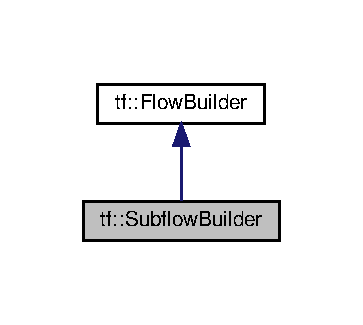
\includegraphics[width=174pt]{classtf_1_1SubflowBuilder__inherit__graph}
\end{center}
\end{figure}


Collaboration diagram for tf\+:\+:Subflow\+Builder\+:\nopagebreak
\begin{figure}[H]
\begin{center}
\leavevmode
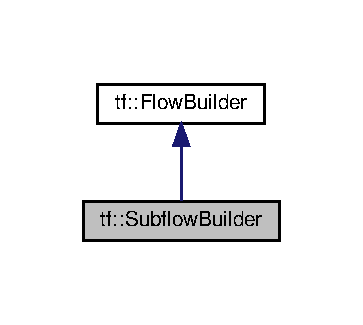
\includegraphics[width=174pt]{classtf_1_1SubflowBuilder__coll__graph}
\end{center}
\end{figure}
\subsection*{Public Member Functions}
\begin{DoxyCompactItemize}
\item 
{\footnotesize template$<$typename... Args$>$ }\\\hyperlink{classtf_1_1SubflowBuilder_a74ae78a9e2f4c3280e39577dffecfbb6}{Subflow\+Builder} (Args \&\&...)
\item 
void \hyperlink{classtf_1_1SubflowBuilder_a10cff676153ad0e83d15a33e8469f59e}{join} ()
\item 
void \hyperlink{classtf_1_1SubflowBuilder_a0660bc0ca5ec375700703cbc94f66942}{detach} ()
\item 
bool \hyperlink{classtf_1_1SubflowBuilder_a39793fbfee4d3fe01541cfd04bf1a5c7}{detached} () const
\item 
bool \hyperlink{classtf_1_1SubflowBuilder_a7e6d76a68180e51cb4108f58a14d5216}{joined} () const
\item 
{\footnotesize template$<$typename... Args$>$ }\\\hyperlink{classtf_1_1SubflowBuilder_a17303b7da88214fa10401d4a3e334070}{Subflow\+Builder} (Args \&\&... args)
\end{DoxyCompactItemize}
\subsection*{Additional Inherited Members}


\subsection{Constructor \& Destructor Documentation}
\mbox{\Hypertarget{classtf_1_1SubflowBuilder_a74ae78a9e2f4c3280e39577dffecfbb6}\label{classtf_1_1SubflowBuilder_a74ae78a9e2f4c3280e39577dffecfbb6}} 
\index{tf\+::\+Subflow\+Builder@{tf\+::\+Subflow\+Builder}!Subflow\+Builder@{Subflow\+Builder}}
\index{Subflow\+Builder@{Subflow\+Builder}!tf\+::\+Subflow\+Builder@{tf\+::\+Subflow\+Builder}}
\subsubsection{\texorpdfstring{Subflow\+Builder()}{SubflowBuilder()}\hspace{0.1cm}{\footnotesize\ttfamily [1/2]}}
{\footnotesize\ttfamily template$<$typename... Args$>$ \\
tf\+::\+Subflow\+Builder\+::\+Subflow\+Builder (\begin{DoxyParamCaption}\item[{Args \&\&}]{... }\end{DoxyParamCaption})}

\mbox{\Hypertarget{classtf_1_1SubflowBuilder_a17303b7da88214fa10401d4a3e334070}\label{classtf_1_1SubflowBuilder_a17303b7da88214fa10401d4a3e334070}} 
\index{tf\+::\+Subflow\+Builder@{tf\+::\+Subflow\+Builder}!Subflow\+Builder@{Subflow\+Builder}}
\index{Subflow\+Builder@{Subflow\+Builder}!tf\+::\+Subflow\+Builder@{tf\+::\+Subflow\+Builder}}
\subsubsection{\texorpdfstring{Subflow\+Builder()}{SubflowBuilder()}\hspace{0.1cm}{\footnotesize\ttfamily [2/2]}}
{\footnotesize\ttfamily template$<$typename... Args$>$ \\
tf\+::\+Subflow\+Builder\+::\+Subflow\+Builder (\begin{DoxyParamCaption}\item[{Args \&\&...}]{args }\end{DoxyParamCaption})}



\subsection{Member Function Documentation}
\mbox{\Hypertarget{classtf_1_1SubflowBuilder_a0660bc0ca5ec375700703cbc94f66942}\label{classtf_1_1SubflowBuilder_a0660bc0ca5ec375700703cbc94f66942}} 
\index{tf\+::\+Subflow\+Builder@{tf\+::\+Subflow\+Builder}!detach@{detach}}
\index{detach@{detach}!tf\+::\+Subflow\+Builder@{tf\+::\+Subflow\+Builder}}
\subsubsection{\texorpdfstring{detach()}{detach()}}
{\footnotesize\ttfamily void tf\+::\+Subflow\+Builder\+::detach (\begin{DoxyParamCaption}{ }\end{DoxyParamCaption})\hspace{0.3cm}{\ttfamily [inline]}}

\mbox{\Hypertarget{classtf_1_1SubflowBuilder_a39793fbfee4d3fe01541cfd04bf1a5c7}\label{classtf_1_1SubflowBuilder_a39793fbfee4d3fe01541cfd04bf1a5c7}} 
\index{tf\+::\+Subflow\+Builder@{tf\+::\+Subflow\+Builder}!detached@{detached}}
\index{detached@{detached}!tf\+::\+Subflow\+Builder@{tf\+::\+Subflow\+Builder}}
\subsubsection{\texorpdfstring{detached()}{detached()}}
{\footnotesize\ttfamily bool tf\+::\+Subflow\+Builder\+::detached (\begin{DoxyParamCaption}{ }\end{DoxyParamCaption}) const\hspace{0.3cm}{\ttfamily [inline]}}

\mbox{\Hypertarget{classtf_1_1SubflowBuilder_a10cff676153ad0e83d15a33e8469f59e}\label{classtf_1_1SubflowBuilder_a10cff676153ad0e83d15a33e8469f59e}} 
\index{tf\+::\+Subflow\+Builder@{tf\+::\+Subflow\+Builder}!join@{join}}
\index{join@{join}!tf\+::\+Subflow\+Builder@{tf\+::\+Subflow\+Builder}}
\subsubsection{\texorpdfstring{join()}{join()}}
{\footnotesize\ttfamily void tf\+::\+Subflow\+Builder\+::join (\begin{DoxyParamCaption}{ }\end{DoxyParamCaption})\hspace{0.3cm}{\ttfamily [inline]}}

\mbox{\Hypertarget{classtf_1_1SubflowBuilder_a7e6d76a68180e51cb4108f58a14d5216}\label{classtf_1_1SubflowBuilder_a7e6d76a68180e51cb4108f58a14d5216}} 
\index{tf\+::\+Subflow\+Builder@{tf\+::\+Subflow\+Builder}!joined@{joined}}
\index{joined@{joined}!tf\+::\+Subflow\+Builder@{tf\+::\+Subflow\+Builder}}
\subsubsection{\texorpdfstring{joined()}{joined()}}
{\footnotesize\ttfamily bool tf\+::\+Subflow\+Builder\+::joined (\begin{DoxyParamCaption}{ }\end{DoxyParamCaption}) const\hspace{0.3cm}{\ttfamily [inline]}}



The documentation for this class was generated from the following file\+:\begin{DoxyCompactItemize}
\item 
/home/twhuang/\+Ph\+D/\+Code/cpp-\/taskflow/taskflow/graph/\hyperlink{flow__builder_8hpp}{flow\+\_\+builder.\+hpp}\end{DoxyCompactItemize}

\hypertarget{classtf_1_1Task}{}\section{tf\+:\+:Task Class Reference}
\label{classtf_1_1Task}\index{tf\+::\+Task@{tf\+::\+Task}}


{\ttfamily \#include $<$graph.\+hpp$>$}

\subsection*{Public Member Functions}
\begin{DoxyCompactItemize}
\item 
\hyperlink{classtf_1_1Task_a5ed7ba63e8eeaa0f21fe08c80aa474ba}{Task} ()=default
\item 
\hyperlink{classtf_1_1Task_ac23878fa7fd15b212e80bcb51e69ce51}{Task} (\hyperlink{classtf_1_1Node}{Node} \&)
\item 
\hyperlink{classtf_1_1Task_a46a1b01af926c0fa699c831073b45f1c}{Task} (const \hyperlink{classtf_1_1Task}{Task} \&)
\item 
\hyperlink{classtf_1_1Task_a4783415f1b49195d34d94def88db5414}{Task} (\hyperlink{classtf_1_1Task}{Task} \&\&)
\item 
\hyperlink{classtf_1_1Task}{Task} \& \hyperlink{classtf_1_1Task_aebdcc47e47a119f261daab673a971458}{operator=} (const \hyperlink{classtf_1_1Task}{Task} \&)
\item 
const std\+::string \& \hyperlink{classtf_1_1Task_a08ada0425b490997b6ff7f310107e5e3}{name} () const
\item 
size\+\_\+t \hyperlink{classtf_1_1Task_a1a0afc89e8a6a416c511e74d82df135d}{num\+\_\+successors} () const
\item 
size\+\_\+t \hyperlink{classtf_1_1Task_a974dc1d738b62b829ad261beeafbd67c}{num\+\_\+dependents} () const
\item 
\hyperlink{classtf_1_1Task}{Task} \& \hyperlink{classtf_1_1Task_a2d3d62a1809d708137763db8e2a8dde8}{name} (const std\+::string \&)
\item 
{\footnotesize template$<$typename C $>$ }\\\hyperlink{classtf_1_1Task}{Task} \& \hyperlink{classtf_1_1Task_a085349bd9ad5066579ce450c7bc78406}{work} (C \&\&)
\item 
{\footnotesize template$<$typename... Ts$>$ }\\\hyperlink{classtf_1_1Task}{Task} \& \hyperlink{classtf_1_1Task_a119a34cce8c92e359f8ed31f2610d0ff}{precede} (Ts \&\&...)
\item 
{\footnotesize template$<$typename... Bs$>$ }\\\hyperlink{classtf_1_1Task}{Task} \& \hyperlink{classtf_1_1Task_a93623de40d7be63008959a0b4dc27e0c}{broadcast} (Bs \&\&...)
\item 
\hyperlink{classtf_1_1Task}{Task} \& \hyperlink{classtf_1_1Task_a533af3422ab292aaa80d55fb2870549d}{broadcast} (std\+::vector$<$ \hyperlink{classtf_1_1Task}{Task} $>$ \&)
\item 
\hyperlink{classtf_1_1Task}{Task} \& \hyperlink{classtf_1_1Task_af53724f41d3b6c7221645bd093d68189}{broadcast} (std\+::initializer\+\_\+list$<$ \hyperlink{classtf_1_1Task}{Task} $>$)
\item 
{\footnotesize template$<$typename... Bs$>$ }\\\hyperlink{classtf_1_1Task}{Task} \& \hyperlink{classtf_1_1Task_aadd7845ba7867a87f1f2ac3f6d7ae569}{gather} (Bs \&\&...)
\item 
\hyperlink{classtf_1_1Task}{Task} \& \hyperlink{classtf_1_1Task_a915feb8a514095f1b98afb857e53e539}{gather} (std\+::vector$<$ \hyperlink{classtf_1_1Task}{Task} $>$ \&)
\item 
\hyperlink{classtf_1_1Task}{Task} \& \hyperlink{classtf_1_1Task_a57a5b65d54bed7e6319500239e35dc19}{gather} (std\+::initializer\+\_\+list$<$ \hyperlink{classtf_1_1Task}{Task} $>$)
\item 
{\footnotesize template$<$typename... Bs$>$ }\\\hyperlink{classtf_1_1Task}{Task} \& \hyperlink{classtf_1_1Task_a5ac7ac1f8f16dc4ec821fa19e36e25b1}{broadcast} (Bs \&\&... tgts)
\item 
{\footnotesize template$<$typename... Ts$>$ }\\\hyperlink{classtf_1_1Task}{Task} \& \hyperlink{classtf_1_1Task_ac8055e2fc0d0a578be87522fff496b55}{precede} (Ts \&\&... tgts)
\item 
{\footnotesize template$<$typename... Bs$>$ }\\\hyperlink{classtf_1_1Task}{Task} \& \hyperlink{classtf_1_1Task_affdecfa1c16d46eb7d8eec1b63e5eed9}{gather} (Bs \&\&... tgts)
\end{DoxyCompactItemize}
\subsection*{Friends}
\begin{DoxyCompactItemize}
\item 
class \hyperlink{classtf_1_1Task_a61184f9bd9c801d0a5eccecfdbddc641}{Flow\+Builder}
\item 
{\footnotesize template$<$template$<$ typename... $>$ typename E$>$ }\\class \hyperlink{classtf_1_1Task_ab3ad8c5c7ed22c3fbd8a41b84db75083}{Basic\+Taskflow}
\end{DoxyCompactItemize}


\subsection{Constructor \& Destructor Documentation}
\mbox{\Hypertarget{classtf_1_1Task_a5ed7ba63e8eeaa0f21fe08c80aa474ba}\label{classtf_1_1Task_a5ed7ba63e8eeaa0f21fe08c80aa474ba}} 
\index{tf\+::\+Task@{tf\+::\+Task}!Task@{Task}}
\index{Task@{Task}!tf\+::\+Task@{tf\+::\+Task}}
\subsubsection{\texorpdfstring{Task()}{Task()}\hspace{0.1cm}{\footnotesize\ttfamily [1/4]}}
{\footnotesize\ttfamily tf\+::\+Task\+::\+Task (\begin{DoxyParamCaption}{ }\end{DoxyParamCaption})\hspace{0.3cm}{\ttfamily [default]}}

\mbox{\Hypertarget{classtf_1_1Task_ac23878fa7fd15b212e80bcb51e69ce51}\label{classtf_1_1Task_ac23878fa7fd15b212e80bcb51e69ce51}} 
\index{tf\+::\+Task@{tf\+::\+Task}!Task@{Task}}
\index{Task@{Task}!tf\+::\+Task@{tf\+::\+Task}}
\subsubsection{\texorpdfstring{Task()}{Task()}\hspace{0.1cm}{\footnotesize\ttfamily [2/4]}}
{\footnotesize\ttfamily tf\+::\+Task\+::\+Task (\begin{DoxyParamCaption}\item[{\hyperlink{classtf_1_1Node}{Node} \&}]{t }\end{DoxyParamCaption})\hspace{0.3cm}{\ttfamily [inline]}}

\mbox{\Hypertarget{classtf_1_1Task_a46a1b01af926c0fa699c831073b45f1c}\label{classtf_1_1Task_a46a1b01af926c0fa699c831073b45f1c}} 
\index{tf\+::\+Task@{tf\+::\+Task}!Task@{Task}}
\index{Task@{Task}!tf\+::\+Task@{tf\+::\+Task}}
\subsubsection{\texorpdfstring{Task()}{Task()}\hspace{0.1cm}{\footnotesize\ttfamily [3/4]}}
{\footnotesize\ttfamily tf\+::\+Task\+::\+Task (\begin{DoxyParamCaption}\item[{const \hyperlink{classtf_1_1Task}{Task} \&}]{rhs }\end{DoxyParamCaption})\hspace{0.3cm}{\ttfamily [inline]}}

\mbox{\Hypertarget{classtf_1_1Task_a4783415f1b49195d34d94def88db5414}\label{classtf_1_1Task_a4783415f1b49195d34d94def88db5414}} 
\index{tf\+::\+Task@{tf\+::\+Task}!Task@{Task}}
\index{Task@{Task}!tf\+::\+Task@{tf\+::\+Task}}
\subsubsection{\texorpdfstring{Task()}{Task()}\hspace{0.1cm}{\footnotesize\ttfamily [4/4]}}
{\footnotesize\ttfamily tf\+::\+Task\+::\+Task (\begin{DoxyParamCaption}\item[{\hyperlink{classtf_1_1Task}{Task} \&\&}]{rhs }\end{DoxyParamCaption})\hspace{0.3cm}{\ttfamily [inline]}}



\subsection{Member Function Documentation}
\mbox{\Hypertarget{classtf_1_1Task_a93623de40d7be63008959a0b4dc27e0c}\label{classtf_1_1Task_a93623de40d7be63008959a0b4dc27e0c}} 
\index{tf\+::\+Task@{tf\+::\+Task}!broadcast@{broadcast}}
\index{broadcast@{broadcast}!tf\+::\+Task@{tf\+::\+Task}}
\subsubsection{\texorpdfstring{broadcast()}{broadcast()}\hspace{0.1cm}{\footnotesize\ttfamily [1/4]}}
{\footnotesize\ttfamily template$<$typename... Bs$>$ \\
\hyperlink{classtf_1_1Task}{Task}\& tf\+::\+Task\+::broadcast (\begin{DoxyParamCaption}\item[{Bs \&\&}]{... }\end{DoxyParamCaption})}

\mbox{\Hypertarget{classtf_1_1Task_a533af3422ab292aaa80d55fb2870549d}\label{classtf_1_1Task_a533af3422ab292aaa80d55fb2870549d}} 
\index{tf\+::\+Task@{tf\+::\+Task}!broadcast@{broadcast}}
\index{broadcast@{broadcast}!tf\+::\+Task@{tf\+::\+Task}}
\subsubsection{\texorpdfstring{broadcast()}{broadcast()}\hspace{0.1cm}{\footnotesize\ttfamily [2/4]}}
{\footnotesize\ttfamily \hyperlink{classtf_1_1Task}{Task} \& tf\+::\+Task\+::broadcast (\begin{DoxyParamCaption}\item[{std\+::vector$<$ \hyperlink{classtf_1_1Task}{Task} $>$ \&}]{tgts }\end{DoxyParamCaption})\hspace{0.3cm}{\ttfamily [inline]}}

\mbox{\Hypertarget{classtf_1_1Task_af53724f41d3b6c7221645bd093d68189}\label{classtf_1_1Task_af53724f41d3b6c7221645bd093d68189}} 
\index{tf\+::\+Task@{tf\+::\+Task}!broadcast@{broadcast}}
\index{broadcast@{broadcast}!tf\+::\+Task@{tf\+::\+Task}}
\subsubsection{\texorpdfstring{broadcast()}{broadcast()}\hspace{0.1cm}{\footnotesize\ttfamily [3/4]}}
{\footnotesize\ttfamily \hyperlink{classtf_1_1Task}{Task} \& tf\+::\+Task\+::broadcast (\begin{DoxyParamCaption}\item[{std\+::initializer\+\_\+list$<$ \hyperlink{classtf_1_1Task}{Task} $>$}]{tgts }\end{DoxyParamCaption})\hspace{0.3cm}{\ttfamily [inline]}}

\mbox{\Hypertarget{classtf_1_1Task_a5ac7ac1f8f16dc4ec821fa19e36e25b1}\label{classtf_1_1Task_a5ac7ac1f8f16dc4ec821fa19e36e25b1}} 
\index{tf\+::\+Task@{tf\+::\+Task}!broadcast@{broadcast}}
\index{broadcast@{broadcast}!tf\+::\+Task@{tf\+::\+Task}}
\subsubsection{\texorpdfstring{broadcast()}{broadcast()}\hspace{0.1cm}{\footnotesize\ttfamily [4/4]}}
{\footnotesize\ttfamily template$<$typename... Bs$>$ \\
\hyperlink{classtf_1_1Task}{Task}\& tf\+::\+Task\+::broadcast (\begin{DoxyParamCaption}\item[{Bs \&\&...}]{tgts }\end{DoxyParamCaption})}

\mbox{\Hypertarget{classtf_1_1Task_aadd7845ba7867a87f1f2ac3f6d7ae569}\label{classtf_1_1Task_aadd7845ba7867a87f1f2ac3f6d7ae569}} 
\index{tf\+::\+Task@{tf\+::\+Task}!gather@{gather}}
\index{gather@{gather}!tf\+::\+Task@{tf\+::\+Task}}
\subsubsection{\texorpdfstring{gather()}{gather()}\hspace{0.1cm}{\footnotesize\ttfamily [1/4]}}
{\footnotesize\ttfamily template$<$typename... Bs$>$ \\
\hyperlink{classtf_1_1Task}{Task}\& tf\+::\+Task\+::gather (\begin{DoxyParamCaption}\item[{Bs \&\&}]{... }\end{DoxyParamCaption})}

\mbox{\Hypertarget{classtf_1_1Task_a915feb8a514095f1b98afb857e53e539}\label{classtf_1_1Task_a915feb8a514095f1b98afb857e53e539}} 
\index{tf\+::\+Task@{tf\+::\+Task}!gather@{gather}}
\index{gather@{gather}!tf\+::\+Task@{tf\+::\+Task}}
\subsubsection{\texorpdfstring{gather()}{gather()}\hspace{0.1cm}{\footnotesize\ttfamily [2/4]}}
{\footnotesize\ttfamily \hyperlink{classtf_1_1Task}{Task} \& tf\+::\+Task\+::gather (\begin{DoxyParamCaption}\item[{std\+::vector$<$ \hyperlink{classtf_1_1Task}{Task} $>$ \&}]{tgts }\end{DoxyParamCaption})\hspace{0.3cm}{\ttfamily [inline]}}

\mbox{\Hypertarget{classtf_1_1Task_a57a5b65d54bed7e6319500239e35dc19}\label{classtf_1_1Task_a57a5b65d54bed7e6319500239e35dc19}} 
\index{tf\+::\+Task@{tf\+::\+Task}!gather@{gather}}
\index{gather@{gather}!tf\+::\+Task@{tf\+::\+Task}}
\subsubsection{\texorpdfstring{gather()}{gather()}\hspace{0.1cm}{\footnotesize\ttfamily [3/4]}}
{\footnotesize\ttfamily \hyperlink{classtf_1_1Task}{Task} \& tf\+::\+Task\+::gather (\begin{DoxyParamCaption}\item[{std\+::initializer\+\_\+list$<$ \hyperlink{classtf_1_1Task}{Task} $>$}]{tgts }\end{DoxyParamCaption})\hspace{0.3cm}{\ttfamily [inline]}}

\mbox{\Hypertarget{classtf_1_1Task_affdecfa1c16d46eb7d8eec1b63e5eed9}\label{classtf_1_1Task_affdecfa1c16d46eb7d8eec1b63e5eed9}} 
\index{tf\+::\+Task@{tf\+::\+Task}!gather@{gather}}
\index{gather@{gather}!tf\+::\+Task@{tf\+::\+Task}}
\subsubsection{\texorpdfstring{gather()}{gather()}\hspace{0.1cm}{\footnotesize\ttfamily [4/4]}}
{\footnotesize\ttfamily template$<$typename... Bs$>$ \\
\hyperlink{classtf_1_1Task}{Task}\& tf\+::\+Task\+::gather (\begin{DoxyParamCaption}\item[{Bs \&\&...}]{tgts }\end{DoxyParamCaption})}

\mbox{\Hypertarget{classtf_1_1Task_a08ada0425b490997b6ff7f310107e5e3}\label{classtf_1_1Task_a08ada0425b490997b6ff7f310107e5e3}} 
\index{tf\+::\+Task@{tf\+::\+Task}!name@{name}}
\index{name@{name}!tf\+::\+Task@{tf\+::\+Task}}
\subsubsection{\texorpdfstring{name()}{name()}\hspace{0.1cm}{\footnotesize\ttfamily [1/2]}}
{\footnotesize\ttfamily const std\+::string \& tf\+::\+Task\+::name (\begin{DoxyParamCaption}{ }\end{DoxyParamCaption}) const\hspace{0.3cm}{\ttfamily [inline]}}

\mbox{\Hypertarget{classtf_1_1Task_a2d3d62a1809d708137763db8e2a8dde8}\label{classtf_1_1Task_a2d3d62a1809d708137763db8e2a8dde8}} 
\index{tf\+::\+Task@{tf\+::\+Task}!name@{name}}
\index{name@{name}!tf\+::\+Task@{tf\+::\+Task}}
\subsubsection{\texorpdfstring{name()}{name()}\hspace{0.1cm}{\footnotesize\ttfamily [2/2]}}
{\footnotesize\ttfamily \hyperlink{classtf_1_1Task}{Task} \& tf\+::\+Task\+::name (\begin{DoxyParamCaption}\item[{const std\+::string \&}]{name }\end{DoxyParamCaption})\hspace{0.3cm}{\ttfamily [inline]}}

\mbox{\Hypertarget{classtf_1_1Task_a974dc1d738b62b829ad261beeafbd67c}\label{classtf_1_1Task_a974dc1d738b62b829ad261beeafbd67c}} 
\index{tf\+::\+Task@{tf\+::\+Task}!num\+\_\+dependents@{num\+\_\+dependents}}
\index{num\+\_\+dependents@{num\+\_\+dependents}!tf\+::\+Task@{tf\+::\+Task}}
\subsubsection{\texorpdfstring{num\+\_\+dependents()}{num\_dependents()}}
{\footnotesize\ttfamily size\+\_\+t tf\+::\+Task\+::num\+\_\+dependents (\begin{DoxyParamCaption}{ }\end{DoxyParamCaption}) const\hspace{0.3cm}{\ttfamily [inline]}}

\mbox{\Hypertarget{classtf_1_1Task_a1a0afc89e8a6a416c511e74d82df135d}\label{classtf_1_1Task_a1a0afc89e8a6a416c511e74d82df135d}} 
\index{tf\+::\+Task@{tf\+::\+Task}!num\+\_\+successors@{num\+\_\+successors}}
\index{num\+\_\+successors@{num\+\_\+successors}!tf\+::\+Task@{tf\+::\+Task}}
\subsubsection{\texorpdfstring{num\+\_\+successors()}{num\_successors()}}
{\footnotesize\ttfamily size\+\_\+t tf\+::\+Task\+::num\+\_\+successors (\begin{DoxyParamCaption}{ }\end{DoxyParamCaption}) const\hspace{0.3cm}{\ttfamily [inline]}}

\mbox{\Hypertarget{classtf_1_1Task_aebdcc47e47a119f261daab673a971458}\label{classtf_1_1Task_aebdcc47e47a119f261daab673a971458}} 
\index{tf\+::\+Task@{tf\+::\+Task}!operator=@{operator=}}
\index{operator=@{operator=}!tf\+::\+Task@{tf\+::\+Task}}
\subsubsection{\texorpdfstring{operator=()}{operator=()}}
{\footnotesize\ttfamily \hyperlink{classtf_1_1Task}{Task} \& tf\+::\+Task\+::operator= (\begin{DoxyParamCaption}\item[{const \hyperlink{classtf_1_1Task}{Task} \&}]{rhs }\end{DoxyParamCaption})\hspace{0.3cm}{\ttfamily [inline]}}

\mbox{\Hypertarget{classtf_1_1Task_a119a34cce8c92e359f8ed31f2610d0ff}\label{classtf_1_1Task_a119a34cce8c92e359f8ed31f2610d0ff}} 
\index{tf\+::\+Task@{tf\+::\+Task}!precede@{precede}}
\index{precede@{precede}!tf\+::\+Task@{tf\+::\+Task}}
\subsubsection{\texorpdfstring{precede()}{precede()}\hspace{0.1cm}{\footnotesize\ttfamily [1/2]}}
{\footnotesize\ttfamily template$<$typename... Ts$>$ \\
\hyperlink{classtf_1_1Task}{Task}\& tf\+::\+Task\+::precede (\begin{DoxyParamCaption}\item[{Ts \&\&}]{... }\end{DoxyParamCaption})}

\mbox{\Hypertarget{classtf_1_1Task_ac8055e2fc0d0a578be87522fff496b55}\label{classtf_1_1Task_ac8055e2fc0d0a578be87522fff496b55}} 
\index{tf\+::\+Task@{tf\+::\+Task}!precede@{precede}}
\index{precede@{precede}!tf\+::\+Task@{tf\+::\+Task}}
\subsubsection{\texorpdfstring{precede()}{precede()}\hspace{0.1cm}{\footnotesize\ttfamily [2/2]}}
{\footnotesize\ttfamily template$<$typename... Ts$>$ \\
\hyperlink{classtf_1_1Task}{Task}\& tf\+::\+Task\+::precede (\begin{DoxyParamCaption}\item[{Ts \&\&...}]{tgts }\end{DoxyParamCaption})}

\mbox{\Hypertarget{classtf_1_1Task_a085349bd9ad5066579ce450c7bc78406}\label{classtf_1_1Task_a085349bd9ad5066579ce450c7bc78406}} 
\index{tf\+::\+Task@{tf\+::\+Task}!work@{work}}
\index{work@{work}!tf\+::\+Task@{tf\+::\+Task}}
\subsubsection{\texorpdfstring{work()}{work()}}
{\footnotesize\ttfamily template$<$typename C $>$ \\
\hyperlink{classtf_1_1Task}{Task} \& tf\+::\+Task\+::work (\begin{DoxyParamCaption}\item[{C \&\&}]{c }\end{DoxyParamCaption})\hspace{0.3cm}{\ttfamily [inline]}}



\subsection{Friends And Related Function Documentation}
\mbox{\Hypertarget{classtf_1_1Task_ab3ad8c5c7ed22c3fbd8a41b84db75083}\label{classtf_1_1Task_ab3ad8c5c7ed22c3fbd8a41b84db75083}} 
\index{tf\+::\+Task@{tf\+::\+Task}!Basic\+Taskflow@{Basic\+Taskflow}}
\index{Basic\+Taskflow@{Basic\+Taskflow}!tf\+::\+Task@{tf\+::\+Task}}
\subsubsection{\texorpdfstring{Basic\+Taskflow}{BasicTaskflow}}
{\footnotesize\ttfamily template$<$template$<$ typename... $>$ typename E$>$ \\
friend class \hyperlink{classtf_1_1BasicTaskflow}{Basic\+Taskflow}\hspace{0.3cm}{\ttfamily [friend]}}

\mbox{\Hypertarget{classtf_1_1Task_a61184f9bd9c801d0a5eccecfdbddc641}\label{classtf_1_1Task_a61184f9bd9c801d0a5eccecfdbddc641}} 
\index{tf\+::\+Task@{tf\+::\+Task}!Flow\+Builder@{Flow\+Builder}}
\index{Flow\+Builder@{Flow\+Builder}!tf\+::\+Task@{tf\+::\+Task}}
\subsubsection{\texorpdfstring{Flow\+Builder}{FlowBuilder}}
{\footnotesize\ttfamily friend class \hyperlink{classtf_1_1FlowBuilder}{Flow\+Builder}\hspace{0.3cm}{\ttfamily [friend]}}



The documentation for this class was generated from the following file\+:\begin{DoxyCompactItemize}
\item 
/home/twhuang/\+Ph\+D/\+Code/cpp-\/taskflow/taskflow/graph/\hyperlink{graph_8hpp}{graph.\+hpp}\end{DoxyCompactItemize}

\hypertarget{classtf_1_1Threadpool}{}\section{tf\+:\+:Threadpool Class Reference}
\label{classtf_1_1Threadpool}\index{tf\+::\+Threadpool@{tf\+::\+Threadpool}}


{\ttfamily \#include $<$threadpool\+\_\+cxx14.\+hpp$>$}

\subsection*{Public Member Functions}
\begin{DoxyCompactItemize}
\item 
\hyperlink{classtf_1_1Threadpool_af2104e27f22728114bca20cce7fc04e0}{Threadpool} (unsigned)
\item 
\hyperlink{classtf_1_1Threadpool_a158e3b7a5f7e36d506fc29f119264014}{$\sim$\+Threadpool} ()
\item 
{\footnotesize template$<$typename C $>$ }\\std\+::enable\+\_\+if\+\_\+t$<$ std\+::is\+\_\+same$<$ void, \hyperlink{namespacestd_a492e7f3c5595a8b7a7c6e0c9294f5c81}{std\+::invoke\+\_\+result\+\_\+t}$<$ C $>$ $>$\+::value, std\+::future$<$ \hyperlink{namespacestd_a492e7f3c5595a8b7a7c6e0c9294f5c81}{std\+::invoke\+\_\+result\+\_\+t}$<$ C $>$ $>$ $>$ \hyperlink{classtf_1_1Threadpool_a0650bfda4fd76f5e8d9d5c35956fbeef}{async} (C \&\&, Signal=Signal\+::\+S\+T\+A\+N\+D\+A\+RD)
\item 
{\footnotesize template$<$typename C $>$ }\\std\+::enable\+\_\+if\+\_\+t$<$ !std\+::is\+\_\+same$<$ void, \hyperlink{namespacestd_a492e7f3c5595a8b7a7c6e0c9294f5c81}{std\+::invoke\+\_\+result\+\_\+t}$<$ C $>$ $>$\+::value, std\+::future$<$ \hyperlink{namespacestd_a492e7f3c5595a8b7a7c6e0c9294f5c81}{std\+::invoke\+\_\+result\+\_\+t}$<$ C $>$ $>$ $>$ \hyperlink{classtf_1_1Threadpool_a6c2cc2938ef035c303d2a43e5c15fcca}{async} (C \&\&, Signal=Signal\+::\+S\+T\+A\+N\+D\+A\+RD)
\item 
{\footnotesize template$<$typename C $>$ }\\auto \hyperlink{classtf_1_1Threadpool_a8d6b238ef8a13beb44e392c1e77e2a43}{silent\+\_\+async} (C \&\&, Signal=Signal\+::\+S\+T\+A\+N\+D\+A\+RD)
\item 
void \hyperlink{classtf_1_1Threadpool_aade7cf005cd323798e34953985515984}{shutdown} ()
\item 
void \hyperlink{classtf_1_1Threadpool_ae80574cb4394509ba3d9b47be20825f5}{spawn} (unsigned)
\item 
void \hyperlink{classtf_1_1Threadpool_ad3c5d9917ee85cb792f464419dceba38}{wait\+\_\+for\+\_\+all} ()
\item 
size\+\_\+t \hyperlink{classtf_1_1Threadpool_ac6b0f5ffa732c877d03a80d40df34455}{num\+\_\+tasks} () const
\item 
size\+\_\+t \hyperlink{classtf_1_1Threadpool_af593a543c7d77229cf9a344b0f15b9f3}{num\+\_\+workers} () const
\item 
bool \hyperlink{classtf_1_1Threadpool_a7aaf377c9298f4b09a59af4a960a32ec}{is\+\_\+worker} () const
\end{DoxyCompactItemize}


\subsection{Constructor \& Destructor Documentation}
\mbox{\Hypertarget{classtf_1_1Threadpool_af2104e27f22728114bca20cce7fc04e0}\label{classtf_1_1Threadpool_af2104e27f22728114bca20cce7fc04e0}} 
\index{tf\+::\+Threadpool@{tf\+::\+Threadpool}!Threadpool@{Threadpool}}
\index{Threadpool@{Threadpool}!tf\+::\+Threadpool@{tf\+::\+Threadpool}}
\subsubsection{\texorpdfstring{Threadpool()}{Threadpool()}}
{\footnotesize\ttfamily tf\+::\+Threadpool\+::\+Threadpool (\begin{DoxyParamCaption}\item[{unsigned}]{N }\end{DoxyParamCaption})\hspace{0.3cm}{\ttfamily [inline]}}

\mbox{\Hypertarget{classtf_1_1Threadpool_a158e3b7a5f7e36d506fc29f119264014}\label{classtf_1_1Threadpool_a158e3b7a5f7e36d506fc29f119264014}} 
\index{tf\+::\+Threadpool@{tf\+::\+Threadpool}!````~Threadpool@{$\sim$\+Threadpool}}
\index{````~Threadpool@{$\sim$\+Threadpool}!tf\+::\+Threadpool@{tf\+::\+Threadpool}}
\subsubsection{\texorpdfstring{$\sim$\+Threadpool()}{~Threadpool()}}
{\footnotesize\ttfamily tf\+::\+Threadpool\+::$\sim$\+Threadpool (\begin{DoxyParamCaption}{ }\end{DoxyParamCaption})\hspace{0.3cm}{\ttfamily [inline]}}



\subsection{Member Function Documentation}
\mbox{\Hypertarget{classtf_1_1Threadpool_a0650bfda4fd76f5e8d9d5c35956fbeef}\label{classtf_1_1Threadpool_a0650bfda4fd76f5e8d9d5c35956fbeef}} 
\index{tf\+::\+Threadpool@{tf\+::\+Threadpool}!async@{async}}
\index{async@{async}!tf\+::\+Threadpool@{tf\+::\+Threadpool}}
\subsubsection{\texorpdfstring{async()}{async()}\hspace{0.1cm}{\footnotesize\ttfamily [1/2]}}
{\footnotesize\ttfamily template$<$typename C $>$ \\
std\+::enable\+\_\+if\+\_\+t$<$ std\+::is\+\_\+same$<$void, \hyperlink{namespacestd_a492e7f3c5595a8b7a7c6e0c9294f5c81}{std\+::invoke\+\_\+result\+\_\+t}$<$C$>$ $>$\+::value, std\+::future$<$\hyperlink{namespacestd_a492e7f3c5595a8b7a7c6e0c9294f5c81}{std\+::invoke\+\_\+result\+\_\+t}$<$C$>$ $>$ $>$ tf\+::\+Threadpool\+::async (\begin{DoxyParamCaption}\item[{C \&\&}]{,  }\item[{Signal}]{ = {\ttfamily Signal\+:\+:STANDARD} }\end{DoxyParamCaption})}

\mbox{\Hypertarget{classtf_1_1Threadpool_a6c2cc2938ef035c303d2a43e5c15fcca}\label{classtf_1_1Threadpool_a6c2cc2938ef035c303d2a43e5c15fcca}} 
\index{tf\+::\+Threadpool@{tf\+::\+Threadpool}!async@{async}}
\index{async@{async}!tf\+::\+Threadpool@{tf\+::\+Threadpool}}
\subsubsection{\texorpdfstring{async()}{async()}\hspace{0.1cm}{\footnotesize\ttfamily [2/2]}}
{\footnotesize\ttfamily template$<$typename C $>$ \\
std\+::enable\+\_\+if\+\_\+t$<$ !std\+::is\+\_\+same$<$void, \hyperlink{namespacestd_a492e7f3c5595a8b7a7c6e0c9294f5c81}{std\+::invoke\+\_\+result\+\_\+t}$<$C$>$ $>$\+::value, std\+::future$<$\hyperlink{namespacestd_a492e7f3c5595a8b7a7c6e0c9294f5c81}{std\+::invoke\+\_\+result\+\_\+t}$<$C$>$ $>$ $>$ tf\+::\+Threadpool\+::async (\begin{DoxyParamCaption}\item[{C \&\&}]{,  }\item[{Signal}]{ = {\ttfamily Signal\+:\+:STANDARD} }\end{DoxyParamCaption})}

\mbox{\Hypertarget{classtf_1_1Threadpool_a7aaf377c9298f4b09a59af4a960a32ec}\label{classtf_1_1Threadpool_a7aaf377c9298f4b09a59af4a960a32ec}} 
\index{tf\+::\+Threadpool@{tf\+::\+Threadpool}!is\+\_\+worker@{is\+\_\+worker}}
\index{is\+\_\+worker@{is\+\_\+worker}!tf\+::\+Threadpool@{tf\+::\+Threadpool}}
\subsubsection{\texorpdfstring{is\+\_\+worker()}{is\_worker()}}
{\footnotesize\ttfamily bool tf\+::\+Threadpool\+::is\+\_\+worker (\begin{DoxyParamCaption}{ }\end{DoxyParamCaption}) const\hspace{0.3cm}{\ttfamily [inline]}}

\mbox{\Hypertarget{classtf_1_1Threadpool_ac6b0f5ffa732c877d03a80d40df34455}\label{classtf_1_1Threadpool_ac6b0f5ffa732c877d03a80d40df34455}} 
\index{tf\+::\+Threadpool@{tf\+::\+Threadpool}!num\+\_\+tasks@{num\+\_\+tasks}}
\index{num\+\_\+tasks@{num\+\_\+tasks}!tf\+::\+Threadpool@{tf\+::\+Threadpool}}
\subsubsection{\texorpdfstring{num\+\_\+tasks()}{num\_tasks()}}
{\footnotesize\ttfamily size\+\_\+t tf\+::\+Threadpool\+::num\+\_\+tasks (\begin{DoxyParamCaption}{ }\end{DoxyParamCaption}) const\hspace{0.3cm}{\ttfamily [inline]}}

\mbox{\Hypertarget{classtf_1_1Threadpool_af593a543c7d77229cf9a344b0f15b9f3}\label{classtf_1_1Threadpool_af593a543c7d77229cf9a344b0f15b9f3}} 
\index{tf\+::\+Threadpool@{tf\+::\+Threadpool}!num\+\_\+workers@{num\+\_\+workers}}
\index{num\+\_\+workers@{num\+\_\+workers}!tf\+::\+Threadpool@{tf\+::\+Threadpool}}
\subsubsection{\texorpdfstring{num\+\_\+workers()}{num\_workers()}}
{\footnotesize\ttfamily size\+\_\+t tf\+::\+Threadpool\+::num\+\_\+workers (\begin{DoxyParamCaption}{ }\end{DoxyParamCaption}) const\hspace{0.3cm}{\ttfamily [inline]}}

\mbox{\Hypertarget{classtf_1_1Threadpool_aade7cf005cd323798e34953985515984}\label{classtf_1_1Threadpool_aade7cf005cd323798e34953985515984}} 
\index{tf\+::\+Threadpool@{tf\+::\+Threadpool}!shutdown@{shutdown}}
\index{shutdown@{shutdown}!tf\+::\+Threadpool@{tf\+::\+Threadpool}}
\subsubsection{\texorpdfstring{shutdown()}{shutdown()}}
{\footnotesize\ttfamily void tf\+::\+Threadpool\+::shutdown (\begin{DoxyParamCaption}{ }\end{DoxyParamCaption})\hspace{0.3cm}{\ttfamily [inline]}}

\mbox{\Hypertarget{classtf_1_1Threadpool_a8d6b238ef8a13beb44e392c1e77e2a43}\label{classtf_1_1Threadpool_a8d6b238ef8a13beb44e392c1e77e2a43}} 
\index{tf\+::\+Threadpool@{tf\+::\+Threadpool}!silent\+\_\+async@{silent\+\_\+async}}
\index{silent\+\_\+async@{silent\+\_\+async}!tf\+::\+Threadpool@{tf\+::\+Threadpool}}
\subsubsection{\texorpdfstring{silent\+\_\+async()}{silent\_async()}}
{\footnotesize\ttfamily template$<$typename C $>$ \\
auto tf\+::\+Threadpool\+::silent\+\_\+async (\begin{DoxyParamCaption}\item[{C \&\&}]{c,  }\item[{Signal}]{sig = {\ttfamily Signal\+:\+:STANDARD} }\end{DoxyParamCaption})}

\mbox{\Hypertarget{classtf_1_1Threadpool_ae80574cb4394509ba3d9b47be20825f5}\label{classtf_1_1Threadpool_ae80574cb4394509ba3d9b47be20825f5}} 
\index{tf\+::\+Threadpool@{tf\+::\+Threadpool}!spawn@{spawn}}
\index{spawn@{spawn}!tf\+::\+Threadpool@{tf\+::\+Threadpool}}
\subsubsection{\texorpdfstring{spawn()}{spawn()}}
{\footnotesize\ttfamily void tf\+::\+Threadpool\+::spawn (\begin{DoxyParamCaption}\item[{unsigned}]{N }\end{DoxyParamCaption})\hspace{0.3cm}{\ttfamily [inline]}}

\mbox{\Hypertarget{classtf_1_1Threadpool_ad3c5d9917ee85cb792f464419dceba38}\label{classtf_1_1Threadpool_ad3c5d9917ee85cb792f464419dceba38}} 
\index{tf\+::\+Threadpool@{tf\+::\+Threadpool}!wait\+\_\+for\+\_\+all@{wait\+\_\+for\+\_\+all}}
\index{wait\+\_\+for\+\_\+all@{wait\+\_\+for\+\_\+all}!tf\+::\+Threadpool@{tf\+::\+Threadpool}}
\subsubsection{\texorpdfstring{wait\+\_\+for\+\_\+all()}{wait\_for\_all()}}
{\footnotesize\ttfamily void tf\+::\+Threadpool\+::wait\+\_\+for\+\_\+all (\begin{DoxyParamCaption}{ }\end{DoxyParamCaption})\hspace{0.3cm}{\ttfamily [inline]}}



The documentation for this class was generated from the following file\+:\begin{DoxyCompactItemize}
\item 
/home/twhuang/\+Ph\+D/\+Code/cpp-\/taskflow/taskflow/threadpool/\hyperlink{threadpool__cxx14_8hpp}{threadpool\+\_\+cxx14.\+hpp}\end{DoxyCompactItemize}

\hypertarget{classtf_1_1Topology}{}\section{tf\+:\+:Topology Class Reference}
\label{classtf_1_1Topology}\index{tf\+::\+Topology@{tf\+::\+Topology}}


{\ttfamily \#include $<$graph.\+hpp$>$}

\subsection*{Public Member Functions}
\begin{DoxyCompactItemize}
\item 
\hyperlink{classtf_1_1Topology_ab0f146309db799239e1e888fd1e13d02}{Topology} (\hyperlink{namespacetf_a2afa7da139285640eaf8122535136dc9}{Graph} \&\&)
\item 
{\footnotesize template$<$typename C $>$ }\\\hyperlink{classtf_1_1Topology_a303fa5fb107070ac5180841c0811cfae}{Topology} (\hyperlink{namespacetf_a2afa7da139285640eaf8122535136dc9}{Graph} \&\&, C \&\&)
\item 
std\+::string \hyperlink{classtf_1_1Topology_a83242ca6b464589d405b9450a418f8ff}{dump} () const
\item 
void \hyperlink{classtf_1_1Topology_a724a982f74804e5ea072845e9c7389a3}{dump} (std\+::ostream \&) const
\end{DoxyCompactItemize}
\subsection*{Friends}
\begin{DoxyCompactItemize}
\item 
{\footnotesize template$<$template$<$ typename... $>$ typename E$>$ }\\class \hyperlink{classtf_1_1Topology_ab3ad8c5c7ed22c3fbd8a41b84db75083}{Basic\+Taskflow}
\end{DoxyCompactItemize}


\subsection{Constructor \& Destructor Documentation}
\mbox{\Hypertarget{classtf_1_1Topology_ab0f146309db799239e1e888fd1e13d02}\label{classtf_1_1Topology_ab0f146309db799239e1e888fd1e13d02}} 
\index{tf\+::\+Topology@{tf\+::\+Topology}!Topology@{Topology}}
\index{Topology@{Topology}!tf\+::\+Topology@{tf\+::\+Topology}}
\subsubsection{\texorpdfstring{Topology()}{Topology()}\hspace{0.1cm}{\footnotesize\ttfamily [1/2]}}
{\footnotesize\ttfamily tf\+::\+Topology\+::\+Topology (\begin{DoxyParamCaption}\item[{\hyperlink{namespacetf_a2afa7da139285640eaf8122535136dc9}{Graph} \&\&}]{t }\end{DoxyParamCaption})\hspace{0.3cm}{\ttfamily [inline]}}

\mbox{\Hypertarget{classtf_1_1Topology_a303fa5fb107070ac5180841c0811cfae}\label{classtf_1_1Topology_a303fa5fb107070ac5180841c0811cfae}} 
\index{tf\+::\+Topology@{tf\+::\+Topology}!Topology@{Topology}}
\index{Topology@{Topology}!tf\+::\+Topology@{tf\+::\+Topology}}
\subsubsection{\texorpdfstring{Topology()}{Topology()}\hspace{0.1cm}{\footnotesize\ttfamily [2/2]}}
{\footnotesize\ttfamily template$<$typename C $>$ \\
tf\+::\+Topology\+::\+Topology (\begin{DoxyParamCaption}\item[{\hyperlink{namespacetf_a2afa7da139285640eaf8122535136dc9}{Graph} \&\&}]{t,  }\item[{C \&\&}]{c }\end{DoxyParamCaption})\hspace{0.3cm}{\ttfamily [inline]}}



\subsection{Member Function Documentation}
\mbox{\Hypertarget{classtf_1_1Topology_a83242ca6b464589d405b9450a418f8ff}\label{classtf_1_1Topology_a83242ca6b464589d405b9450a418f8ff}} 
\index{tf\+::\+Topology@{tf\+::\+Topology}!dump@{dump}}
\index{dump@{dump}!tf\+::\+Topology@{tf\+::\+Topology}}
\subsubsection{\texorpdfstring{dump()}{dump()}\hspace{0.1cm}{\footnotesize\ttfamily [1/2]}}
{\footnotesize\ttfamily std\+::string tf\+::\+Topology\+::dump (\begin{DoxyParamCaption}{ }\end{DoxyParamCaption}) const\hspace{0.3cm}{\ttfamily [inline]}}

\mbox{\Hypertarget{classtf_1_1Topology_a724a982f74804e5ea072845e9c7389a3}\label{classtf_1_1Topology_a724a982f74804e5ea072845e9c7389a3}} 
\index{tf\+::\+Topology@{tf\+::\+Topology}!dump@{dump}}
\index{dump@{dump}!tf\+::\+Topology@{tf\+::\+Topology}}
\subsubsection{\texorpdfstring{dump()}{dump()}\hspace{0.1cm}{\footnotesize\ttfamily [2/2]}}
{\footnotesize\ttfamily void tf\+::\+Topology\+::dump (\begin{DoxyParamCaption}\item[{std\+::ostream \&}]{os }\end{DoxyParamCaption}) const\hspace{0.3cm}{\ttfamily [inline]}}



\subsection{Friends And Related Function Documentation}
\mbox{\Hypertarget{classtf_1_1Topology_ab3ad8c5c7ed22c3fbd8a41b84db75083}\label{classtf_1_1Topology_ab3ad8c5c7ed22c3fbd8a41b84db75083}} 
\index{tf\+::\+Topology@{tf\+::\+Topology}!Basic\+Taskflow@{Basic\+Taskflow}}
\index{Basic\+Taskflow@{Basic\+Taskflow}!tf\+::\+Topology@{tf\+::\+Topology}}
\subsubsection{\texorpdfstring{Basic\+Taskflow}{BasicTaskflow}}
{\footnotesize\ttfamily template$<$template$<$ typename... $>$ typename E$>$ \\
friend class \hyperlink{classtf_1_1BasicTaskflow}{Basic\+Taskflow}\hspace{0.3cm}{\ttfamily [friend]}}



The documentation for this class was generated from the following file\+:\begin{DoxyCompactItemize}
\item 
/home/twhuang/\+Ph\+D/\+Code/cpp-\/taskflow/taskflow/graph/\hyperlink{graph_8hpp}{graph.\+hpp}\end{DoxyCompactItemize}

\hypertarget{classtf_1_1WorkStealingQueue}{}\section{tf\+:\+:Work\+Stealing\+Queue$<$ T $>$ Class Template Reference}
\label{classtf_1_1WorkStealingQueue}\index{tf\+::\+Work\+Stealing\+Queue$<$ T $>$@{tf\+::\+Work\+Stealing\+Queue$<$ T $>$}}


{\ttfamily \#include $<$workstealing\+\_\+threadpool.\+hpp$>$}

\subsection*{Public Member Functions}
\begin{DoxyCompactItemize}
\item 
\hyperlink{classtf_1_1WorkStealingQueue_aa55d570fe0d29d68f080c328218a0421}{Work\+Stealing\+Queue} (int64\+\_\+t=4096)
\item 
\hyperlink{classtf_1_1WorkStealingQueue_acb22a49430fd235aa2ae4770d1cd662b}{$\sim$\+Work\+Stealing\+Queue} ()
\item 
bool \hyperlink{classtf_1_1WorkStealingQueue_adc85682657a3cd6c0fe87a71d350036c}{empty} () const noexcept
\item 
int64\+\_\+t \hyperlink{classtf_1_1WorkStealingQueue_aada5323cb64e23796df418c5be124b29}{size} () const noexcept
\item 
int64\+\_\+t \hyperlink{classtf_1_1WorkStealingQueue_aa24605d46953ae1d27dd35451c72c9b3}{capacity} () const noexcept
\item 
{\footnotesize template$<$typename O $>$ }\\void \hyperlink{classtf_1_1WorkStealingQueue_a0d2632d5fbff766101df431b365790c0}{push} (O \&\&)
\item 
std\+::optional$<$ T $>$ \hyperlink{classtf_1_1WorkStealingQueue_a1ba75ce446b149de97e62310851a243d}{pop} ()
\item 
std\+::optional$<$ T $>$ \hyperlink{classtf_1_1WorkStealingQueue_a6b63dca550a2f576b92f05bdc2e03a74}{steal} ()
\end{DoxyCompactItemize}


\subsection{Constructor \& Destructor Documentation}
\mbox{\Hypertarget{classtf_1_1WorkStealingQueue_aa55d570fe0d29d68f080c328218a0421}\label{classtf_1_1WorkStealingQueue_aa55d570fe0d29d68f080c328218a0421}} 
\index{tf\+::\+Work\+Stealing\+Queue@{tf\+::\+Work\+Stealing\+Queue}!Work\+Stealing\+Queue@{Work\+Stealing\+Queue}}
\index{Work\+Stealing\+Queue@{Work\+Stealing\+Queue}!tf\+::\+Work\+Stealing\+Queue@{tf\+::\+Work\+Stealing\+Queue}}
\subsubsection{\texorpdfstring{Work\+Stealing\+Queue()}{WorkStealingQueue()}}
{\footnotesize\ttfamily template$<$typename T $>$ \\
\hyperlink{classtf_1_1WorkStealingQueue}{tf\+::\+Work\+Stealing\+Queue}$<$ T $>$\+::\hyperlink{classtf_1_1WorkStealingQueue}{Work\+Stealing\+Queue} (\begin{DoxyParamCaption}\item[{int64\+\_\+t}]{c = {\ttfamily 4096} }\end{DoxyParamCaption})}

\mbox{\Hypertarget{classtf_1_1WorkStealingQueue_acb22a49430fd235aa2ae4770d1cd662b}\label{classtf_1_1WorkStealingQueue_acb22a49430fd235aa2ae4770d1cd662b}} 
\index{tf\+::\+Work\+Stealing\+Queue@{tf\+::\+Work\+Stealing\+Queue}!````~Work\+Stealing\+Queue@{$\sim$\+Work\+Stealing\+Queue}}
\index{````~Work\+Stealing\+Queue@{$\sim$\+Work\+Stealing\+Queue}!tf\+::\+Work\+Stealing\+Queue@{tf\+::\+Work\+Stealing\+Queue}}
\subsubsection{\texorpdfstring{$\sim$\+Work\+Stealing\+Queue()}{~WorkStealingQueue()}}
{\footnotesize\ttfamily template$<$typename T $>$ \\
\hyperlink{classtf_1_1WorkStealingQueue}{tf\+::\+Work\+Stealing\+Queue}$<$ T $>$\+::$\sim$\hyperlink{classtf_1_1WorkStealingQueue}{Work\+Stealing\+Queue} (\begin{DoxyParamCaption}{ }\end{DoxyParamCaption})}



\subsection{Member Function Documentation}
\mbox{\Hypertarget{classtf_1_1WorkStealingQueue_aa24605d46953ae1d27dd35451c72c9b3}\label{classtf_1_1WorkStealingQueue_aa24605d46953ae1d27dd35451c72c9b3}} 
\index{tf\+::\+Work\+Stealing\+Queue@{tf\+::\+Work\+Stealing\+Queue}!capacity@{capacity}}
\index{capacity@{capacity}!tf\+::\+Work\+Stealing\+Queue@{tf\+::\+Work\+Stealing\+Queue}}
\subsubsection{\texorpdfstring{capacity()}{capacity()}}
{\footnotesize\ttfamily template$<$typename T $>$ \\
int64\+\_\+t \hyperlink{classtf_1_1WorkStealingQueue}{tf\+::\+Work\+Stealing\+Queue}$<$ T $>$\+::capacity (\begin{DoxyParamCaption}{ }\end{DoxyParamCaption}) const\hspace{0.3cm}{\ttfamily [noexcept]}}

\mbox{\Hypertarget{classtf_1_1WorkStealingQueue_adc85682657a3cd6c0fe87a71d350036c}\label{classtf_1_1WorkStealingQueue_adc85682657a3cd6c0fe87a71d350036c}} 
\index{tf\+::\+Work\+Stealing\+Queue@{tf\+::\+Work\+Stealing\+Queue}!empty@{empty}}
\index{empty@{empty}!tf\+::\+Work\+Stealing\+Queue@{tf\+::\+Work\+Stealing\+Queue}}
\subsubsection{\texorpdfstring{empty()}{empty()}}
{\footnotesize\ttfamily template$<$typename T $>$ \\
bool \hyperlink{classtf_1_1WorkStealingQueue}{tf\+::\+Work\+Stealing\+Queue}$<$ T $>$\+::empty (\begin{DoxyParamCaption}{ }\end{DoxyParamCaption}) const\hspace{0.3cm}{\ttfamily [noexcept]}}

\mbox{\Hypertarget{classtf_1_1WorkStealingQueue_a1ba75ce446b149de97e62310851a243d}\label{classtf_1_1WorkStealingQueue_a1ba75ce446b149de97e62310851a243d}} 
\index{tf\+::\+Work\+Stealing\+Queue@{tf\+::\+Work\+Stealing\+Queue}!pop@{pop}}
\index{pop@{pop}!tf\+::\+Work\+Stealing\+Queue@{tf\+::\+Work\+Stealing\+Queue}}
\subsubsection{\texorpdfstring{pop()}{pop()}}
{\footnotesize\ttfamily template$<$typename T $>$ \\
std\+::optional$<$ T $>$ \hyperlink{classtf_1_1WorkStealingQueue}{tf\+::\+Work\+Stealing\+Queue}$<$ T $>$\+::pop (\begin{DoxyParamCaption}{ }\end{DoxyParamCaption})}

\mbox{\Hypertarget{classtf_1_1WorkStealingQueue_a0d2632d5fbff766101df431b365790c0}\label{classtf_1_1WorkStealingQueue_a0d2632d5fbff766101df431b365790c0}} 
\index{tf\+::\+Work\+Stealing\+Queue@{tf\+::\+Work\+Stealing\+Queue}!push@{push}}
\index{push@{push}!tf\+::\+Work\+Stealing\+Queue@{tf\+::\+Work\+Stealing\+Queue}}
\subsubsection{\texorpdfstring{push()}{push()}}
{\footnotesize\ttfamily template$<$typename T $>$ \\
template$<$typename O $>$ \\
void \hyperlink{classtf_1_1WorkStealingQueue}{tf\+::\+Work\+Stealing\+Queue}$<$ T $>$\+::push (\begin{DoxyParamCaption}\item[{O \&\&}]{o }\end{DoxyParamCaption})}

\mbox{\Hypertarget{classtf_1_1WorkStealingQueue_aada5323cb64e23796df418c5be124b29}\label{classtf_1_1WorkStealingQueue_aada5323cb64e23796df418c5be124b29}} 
\index{tf\+::\+Work\+Stealing\+Queue@{tf\+::\+Work\+Stealing\+Queue}!size@{size}}
\index{size@{size}!tf\+::\+Work\+Stealing\+Queue@{tf\+::\+Work\+Stealing\+Queue}}
\subsubsection{\texorpdfstring{size()}{size()}}
{\footnotesize\ttfamily template$<$typename T $>$ \\
int64\+\_\+t \hyperlink{classtf_1_1WorkStealingQueue}{tf\+::\+Work\+Stealing\+Queue}$<$ T $>$\+::size (\begin{DoxyParamCaption}{ }\end{DoxyParamCaption}) const\hspace{0.3cm}{\ttfamily [noexcept]}}

\mbox{\Hypertarget{classtf_1_1WorkStealingQueue_a6b63dca550a2f576b92f05bdc2e03a74}\label{classtf_1_1WorkStealingQueue_a6b63dca550a2f576b92f05bdc2e03a74}} 
\index{tf\+::\+Work\+Stealing\+Queue@{tf\+::\+Work\+Stealing\+Queue}!steal@{steal}}
\index{steal@{steal}!tf\+::\+Work\+Stealing\+Queue@{tf\+::\+Work\+Stealing\+Queue}}
\subsubsection{\texorpdfstring{steal()}{steal()}}
{\footnotesize\ttfamily template$<$typename T $>$ \\
std\+::optional$<$ T $>$ \hyperlink{classtf_1_1WorkStealingQueue}{tf\+::\+Work\+Stealing\+Queue}$<$ T $>$\+::steal (\begin{DoxyParamCaption}{ }\end{DoxyParamCaption})}



The documentation for this class was generated from the following file\+:\begin{DoxyCompactItemize}
\item 
/home/twhuang/\+Ph\+D/\+Code/cpp-\/taskflow/taskflow/threadpool/\hyperlink{workstealing__threadpool_8hpp}{workstealing\+\_\+threadpool.\+hpp}\end{DoxyCompactItemize}

\hypertarget{classtf_1_1WorkStealingThreadpool}{}\section{tf\+:\+:Work\+Stealing\+Threadpool$<$ Closure $>$ Class Template Reference}
\label{classtf_1_1WorkStealingThreadpool}\index{tf\+::\+Work\+Stealing\+Threadpool$<$ Closure $>$@{tf\+::\+Work\+Stealing\+Threadpool$<$ Closure $>$}}


{\ttfamily \#include $<$workstealing\+\_\+threadpool.\+hpp$>$}

\subsection*{Public Member Functions}
\begin{DoxyCompactItemize}
\item 
\hyperlink{classtf_1_1WorkStealingThreadpool_a9069a604b03e3f4abd3f9e4668131581}{Work\+Stealing\+Threadpool} (unsigned)
\item 
\hyperlink{classtf_1_1WorkStealingThreadpool_aa18a26ff7202b289b983ce960d4ff5b9}{$\sim$\+Work\+Stealing\+Threadpool} ()
\item 
size\+\_\+t \hyperlink{classtf_1_1WorkStealingThreadpool_a8fab9139bf428a30f0be2b459f7a82ce}{num\+\_\+tasks} () const
\item 
size\+\_\+t \hyperlink{classtf_1_1WorkStealingThreadpool_a0069de0539feee6c7b211662211a81cc}{num\+\_\+workers} () const
\item 
bool \hyperlink{classtf_1_1WorkStealingThreadpool_ab9d2bb67582347321e44e98fa7bb95cc}{is\+\_\+owner} () const
\item 
{\footnotesize template$<$typename... ArgsT$>$ }\\void \hyperlink{classtf_1_1WorkStealingThreadpool_acdd4b5561fe85f1baa0afb9fd936116f}{emplace} (ArgsT \&\&...)
\item 
void \hyperlink{classtf_1_1WorkStealingThreadpool_af8aea2f24e9dd9de605080472568e644}{batch} (std\+::vector$<$ Closure $>$ \&\&)
\item 
{\footnotesize template$<$typename... ArgsT$>$ }\\void \hyperlink{classtf_1_1WorkStealingThreadpool_afc34fd5581ae10fe53bb2e388f6b9237}{emplace} (ArgsT \&\&... args)
\end{DoxyCompactItemize}


\subsection{Constructor \& Destructor Documentation}
\mbox{\Hypertarget{classtf_1_1WorkStealingThreadpool_a9069a604b03e3f4abd3f9e4668131581}\label{classtf_1_1WorkStealingThreadpool_a9069a604b03e3f4abd3f9e4668131581}} 
\index{tf\+::\+Work\+Stealing\+Threadpool@{tf\+::\+Work\+Stealing\+Threadpool}!Work\+Stealing\+Threadpool@{Work\+Stealing\+Threadpool}}
\index{Work\+Stealing\+Threadpool@{Work\+Stealing\+Threadpool}!tf\+::\+Work\+Stealing\+Threadpool@{tf\+::\+Work\+Stealing\+Threadpool}}
\subsubsection{\texorpdfstring{Work\+Stealing\+Threadpool()}{WorkStealingThreadpool()}}
{\footnotesize\ttfamily template$<$typename Closure $>$ \\
\hyperlink{classtf_1_1WorkStealingThreadpool}{tf\+::\+Work\+Stealing\+Threadpool}$<$ Closure $>$\+::\hyperlink{classtf_1_1WorkStealingThreadpool}{Work\+Stealing\+Threadpool} (\begin{DoxyParamCaption}\item[{unsigned}]{N }\end{DoxyParamCaption})}

\mbox{\Hypertarget{classtf_1_1WorkStealingThreadpool_aa18a26ff7202b289b983ce960d4ff5b9}\label{classtf_1_1WorkStealingThreadpool_aa18a26ff7202b289b983ce960d4ff5b9}} 
\index{tf\+::\+Work\+Stealing\+Threadpool@{tf\+::\+Work\+Stealing\+Threadpool}!````~Work\+Stealing\+Threadpool@{$\sim$\+Work\+Stealing\+Threadpool}}
\index{````~Work\+Stealing\+Threadpool@{$\sim$\+Work\+Stealing\+Threadpool}!tf\+::\+Work\+Stealing\+Threadpool@{tf\+::\+Work\+Stealing\+Threadpool}}
\subsubsection{\texorpdfstring{$\sim$\+Work\+Stealing\+Threadpool()}{~WorkStealingThreadpool()}}
{\footnotesize\ttfamily template$<$typename Closure $>$ \\
\hyperlink{classtf_1_1WorkStealingThreadpool}{tf\+::\+Work\+Stealing\+Threadpool}$<$ Closure $>$\+::$\sim$\hyperlink{classtf_1_1WorkStealingThreadpool}{Work\+Stealing\+Threadpool} (\begin{DoxyParamCaption}{ }\end{DoxyParamCaption})}



\subsection{Member Function Documentation}
\mbox{\Hypertarget{classtf_1_1WorkStealingThreadpool_af8aea2f24e9dd9de605080472568e644}\label{classtf_1_1WorkStealingThreadpool_af8aea2f24e9dd9de605080472568e644}} 
\index{tf\+::\+Work\+Stealing\+Threadpool@{tf\+::\+Work\+Stealing\+Threadpool}!batch@{batch}}
\index{batch@{batch}!tf\+::\+Work\+Stealing\+Threadpool@{tf\+::\+Work\+Stealing\+Threadpool}}
\subsubsection{\texorpdfstring{batch()}{batch()}}
{\footnotesize\ttfamily template$<$typename Closure $>$ \\
void \hyperlink{classtf_1_1WorkStealingThreadpool}{tf\+::\+Work\+Stealing\+Threadpool}$<$ Closure $>$\+::batch (\begin{DoxyParamCaption}\item[{std\+::vector$<$ Closure $>$ \&\&}]{tasks }\end{DoxyParamCaption})}

\mbox{\Hypertarget{classtf_1_1WorkStealingThreadpool_acdd4b5561fe85f1baa0afb9fd936116f}\label{classtf_1_1WorkStealingThreadpool_acdd4b5561fe85f1baa0afb9fd936116f}} 
\index{tf\+::\+Work\+Stealing\+Threadpool@{tf\+::\+Work\+Stealing\+Threadpool}!emplace@{emplace}}
\index{emplace@{emplace}!tf\+::\+Work\+Stealing\+Threadpool@{tf\+::\+Work\+Stealing\+Threadpool}}
\subsubsection{\texorpdfstring{emplace()}{emplace()}\hspace{0.1cm}{\footnotesize\ttfamily [1/2]}}
{\footnotesize\ttfamily template$<$typename Closure $>$ \\
template$<$typename... ArgsT$>$ \\
void \hyperlink{classtf_1_1WorkStealingThreadpool}{tf\+::\+Work\+Stealing\+Threadpool}$<$ Closure $>$\+::emplace (\begin{DoxyParamCaption}\item[{ArgsT \&\&}]{... }\end{DoxyParamCaption})}

\mbox{\Hypertarget{classtf_1_1WorkStealingThreadpool_afc34fd5581ae10fe53bb2e388f6b9237}\label{classtf_1_1WorkStealingThreadpool_afc34fd5581ae10fe53bb2e388f6b9237}} 
\index{tf\+::\+Work\+Stealing\+Threadpool@{tf\+::\+Work\+Stealing\+Threadpool}!emplace@{emplace}}
\index{emplace@{emplace}!tf\+::\+Work\+Stealing\+Threadpool@{tf\+::\+Work\+Stealing\+Threadpool}}
\subsubsection{\texorpdfstring{emplace()}{emplace()}\hspace{0.1cm}{\footnotesize\ttfamily [2/2]}}
{\footnotesize\ttfamily template$<$typename Closure $>$ \\
template$<$typename... ArgsT$>$ \\
void \hyperlink{classtf_1_1WorkStealingThreadpool}{tf\+::\+Work\+Stealing\+Threadpool}$<$ Closure $>$\+::emplace (\begin{DoxyParamCaption}\item[{ArgsT \&\&...}]{args }\end{DoxyParamCaption})}

\mbox{\Hypertarget{classtf_1_1WorkStealingThreadpool_ab9d2bb67582347321e44e98fa7bb95cc}\label{classtf_1_1WorkStealingThreadpool_ab9d2bb67582347321e44e98fa7bb95cc}} 
\index{tf\+::\+Work\+Stealing\+Threadpool@{tf\+::\+Work\+Stealing\+Threadpool}!is\+\_\+owner@{is\+\_\+owner}}
\index{is\+\_\+owner@{is\+\_\+owner}!tf\+::\+Work\+Stealing\+Threadpool@{tf\+::\+Work\+Stealing\+Threadpool}}
\subsubsection{\texorpdfstring{is\+\_\+owner()}{is\_owner()}}
{\footnotesize\ttfamily template$<$typename Closure $>$ \\
bool \hyperlink{classtf_1_1WorkStealingThreadpool}{tf\+::\+Work\+Stealing\+Threadpool}$<$ Closure $>$\+::is\+\_\+owner (\begin{DoxyParamCaption}{ }\end{DoxyParamCaption}) const}

\mbox{\Hypertarget{classtf_1_1WorkStealingThreadpool_a8fab9139bf428a30f0be2b459f7a82ce}\label{classtf_1_1WorkStealingThreadpool_a8fab9139bf428a30f0be2b459f7a82ce}} 
\index{tf\+::\+Work\+Stealing\+Threadpool@{tf\+::\+Work\+Stealing\+Threadpool}!num\+\_\+tasks@{num\+\_\+tasks}}
\index{num\+\_\+tasks@{num\+\_\+tasks}!tf\+::\+Work\+Stealing\+Threadpool@{tf\+::\+Work\+Stealing\+Threadpool}}
\subsubsection{\texorpdfstring{num\+\_\+tasks()}{num\_tasks()}}
{\footnotesize\ttfamily template$<$typename Closure $>$ \\
size\+\_\+t \hyperlink{classtf_1_1WorkStealingThreadpool}{tf\+::\+Work\+Stealing\+Threadpool}$<$ Closure $>$\+::num\+\_\+tasks (\begin{DoxyParamCaption}{ }\end{DoxyParamCaption}) const}

\mbox{\Hypertarget{classtf_1_1WorkStealingThreadpool_a0069de0539feee6c7b211662211a81cc}\label{classtf_1_1WorkStealingThreadpool_a0069de0539feee6c7b211662211a81cc}} 
\index{tf\+::\+Work\+Stealing\+Threadpool@{tf\+::\+Work\+Stealing\+Threadpool}!num\+\_\+workers@{num\+\_\+workers}}
\index{num\+\_\+workers@{num\+\_\+workers}!tf\+::\+Work\+Stealing\+Threadpool@{tf\+::\+Work\+Stealing\+Threadpool}}
\subsubsection{\texorpdfstring{num\+\_\+workers()}{num\_workers()}}
{\footnotesize\ttfamily template$<$typename Closure $>$ \\
size\+\_\+t \hyperlink{classtf_1_1WorkStealingThreadpool}{tf\+::\+Work\+Stealing\+Threadpool}$<$ Closure $>$\+::num\+\_\+workers (\begin{DoxyParamCaption}{ }\end{DoxyParamCaption}) const}



The documentation for this class was generated from the following file\+:\begin{DoxyCompactItemize}
\item 
/home/twhuang/\+Ph\+D/\+Code/cpp-\/taskflow/taskflow/threadpool/\hyperlink{workstealing__threadpool_8hpp}{workstealing\+\_\+threadpool.\+hpp}\end{DoxyCompactItemize}

\chapter{File Documentation}
\hypertarget{error_8hpp}{}\section{/home/twhuang/\+Ph\+D/\+Code/cpp-\/taskflow/taskflow/error/error.hpp File Reference}
\label{error_8hpp}\index{/home/twhuang/\+Ph\+D/\+Code/cpp-\/taskflow/taskflow/error/error.\+hpp@{/home/twhuang/\+Ph\+D/\+Code/cpp-\/taskflow/taskflow/error/error.\+hpp}}
{\ttfamily \#include $<$iostream$>$}\newline
{\ttfamily \#include $<$sstream$>$}\newline
{\ttfamily \#include $<$exception$>$}\newline
{\ttfamily \#include $<$system\+\_\+error$>$}\newline
Include dependency graph for error.\+hpp\+:\nopagebreak
\begin{figure}[H]
\begin{center}
\leavevmode
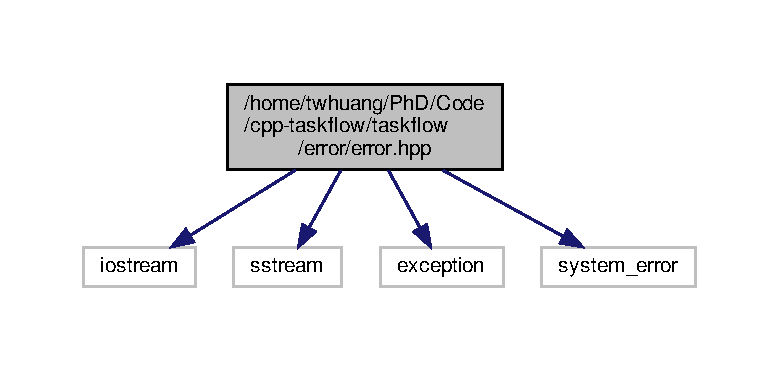
\includegraphics[width=350pt]{error_8hpp__incl}
\end{center}
\end{figure}
This graph shows which files directly or indirectly include this file\+:\nopagebreak
\begin{figure}[H]
\begin{center}
\leavevmode
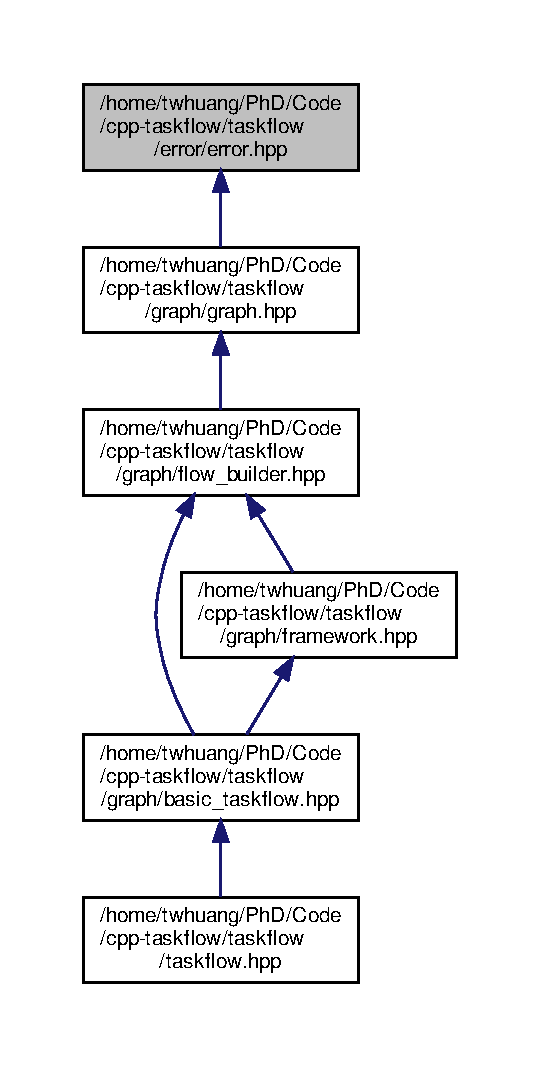
\includegraphics[width=259pt]{error_8hpp__dep__incl}
\end{center}
\end{figure}
\subsection*{Classes}
\begin{DoxyCompactItemize}
\item 
struct \hyperlink{structtf_1_1Error}{tf\+::\+Error}
\item 
struct \hyperlink{structstd_1_1is__error__code__enum_3_01tf_1_1Error_1_1Code_01_4}{std\+::is\+\_\+error\+\_\+code\+\_\+enum$<$ tf\+::\+Error\+::\+Code $>$}
\end{DoxyCompactItemize}
\subsection*{Namespaces}
\begin{DoxyCompactItemize}
\item 
 \hyperlink{namespacetf}{tf}
\item 
 \hyperlink{namespacestd}{std}
\end{DoxyCompactItemize}
\subsection*{Macros}
\begin{DoxyCompactItemize}
\item 
\#define \hyperlink{error_8hpp_aecd66f17d01de60aeb9cae992c9dd4bf}{T\+F\+\_\+\+T\+H\+R\+OW}(...)~\hyperlink{namespacetf_ab9d4e31acc93431725fa1affca09e823}{tf\+::throw\+\_\+se}(\+\_\+\+\_\+\+F\+I\+L\+E\+\_\+\+\_\+, \+\_\+\+\_\+\+L\+I\+N\+E\+\_\+\+\_\+, \+\_\+\+\_\+\+V\+A\+\_\+\+A\+R\+G\+S\+\_\+\+\_\+);
\end{DoxyCompactItemize}
\subsection*{Functions}
\begin{DoxyCompactItemize}
\item 
std\+::error\+\_\+code \hyperlink{namespacetf_aba49ed1abcd24ee88f72374c706c3b87}{tf\+::make\+\_\+error\+\_\+code} (Error\+::\+Code e)
\item 
{\footnotesize template$<$typename... ArgsT$>$ }\\void \hyperlink{namespacetf_ab9d4e31acc93431725fa1affca09e823}{tf\+::throw\+\_\+se} (const char $\ast$fname, const size\+\_\+t line, Error\+::\+Code c, ArgsT \&\&... args)
\end{DoxyCompactItemize}


\subsection{Macro Definition Documentation}
\mbox{\Hypertarget{error_8hpp_aecd66f17d01de60aeb9cae992c9dd4bf}\label{error_8hpp_aecd66f17d01de60aeb9cae992c9dd4bf}} 
\index{error.\+hpp@{error.\+hpp}!T\+F\+\_\+\+T\+H\+R\+OW@{T\+F\+\_\+\+T\+H\+R\+OW}}
\index{T\+F\+\_\+\+T\+H\+R\+OW@{T\+F\+\_\+\+T\+H\+R\+OW}!error.\+hpp@{error.\+hpp}}
\subsubsection{\texorpdfstring{T\+F\+\_\+\+T\+H\+R\+OW}{TF\_THROW}}
{\footnotesize\ttfamily \#define T\+F\+\_\+\+T\+H\+R\+OW(\begin{DoxyParamCaption}\item[{}]{... }\end{DoxyParamCaption})~\hyperlink{namespacetf_ab9d4e31acc93431725fa1affca09e823}{tf\+::throw\+\_\+se}(\+\_\+\+\_\+\+F\+I\+L\+E\+\_\+\+\_\+, \+\_\+\+\_\+\+L\+I\+N\+E\+\_\+\+\_\+, \+\_\+\+\_\+\+V\+A\+\_\+\+A\+R\+G\+S\+\_\+\+\_\+);}


\hypertarget{basic__taskflow_8hpp}{}\section{/home/twhuang/\+Ph\+D/\+Code/cpp-\/taskflow/taskflow/graph/basic\+\_\+taskflow.hpp File Reference}
\label{basic__taskflow_8hpp}\index{/home/twhuang/\+Ph\+D/\+Code/cpp-\/taskflow/taskflow/graph/basic\+\_\+taskflow.\+hpp@{/home/twhuang/\+Ph\+D/\+Code/cpp-\/taskflow/taskflow/graph/basic\+\_\+taskflow.\+hpp}}
{\ttfamily \#include \char`\"{}../threadpool/threadpool.\+hpp\char`\"{}}\newline
{\ttfamily \#include \char`\"{}flow\+\_\+builder.\+hpp\char`\"{}}\newline
{\ttfamily \#include \char`\"{}framework.\+hpp\char`\"{}}\newline
Include dependency graph for basic\+\_\+taskflow.\+hpp\+:\nopagebreak
\begin{figure}[H]
\begin{center}
\leavevmode
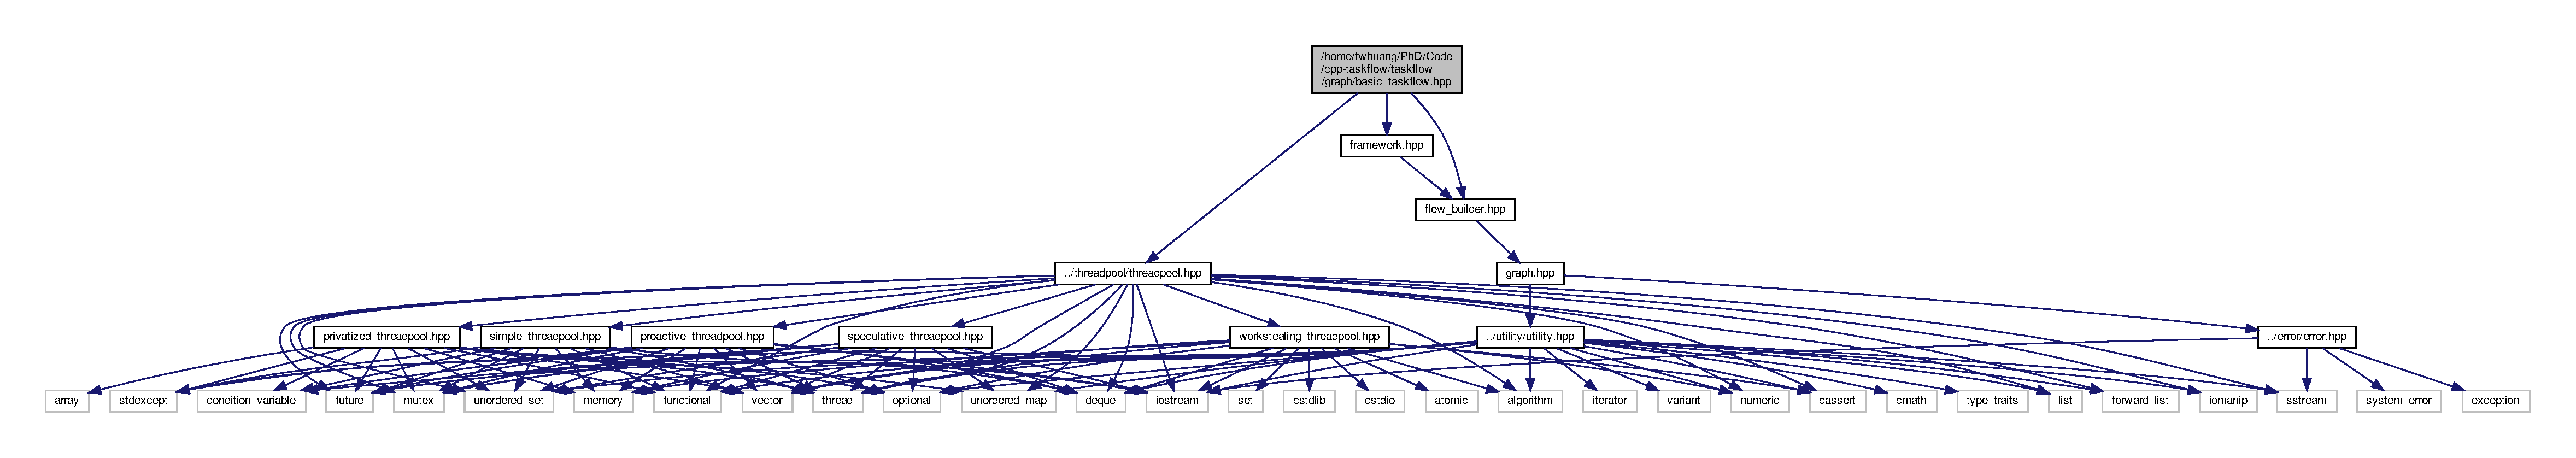
\includegraphics[width=350pt]{basic__taskflow_8hpp__incl}
\end{center}
\end{figure}
This graph shows which files directly or indirectly include this file\+:\nopagebreak
\begin{figure}[H]
\begin{center}
\leavevmode
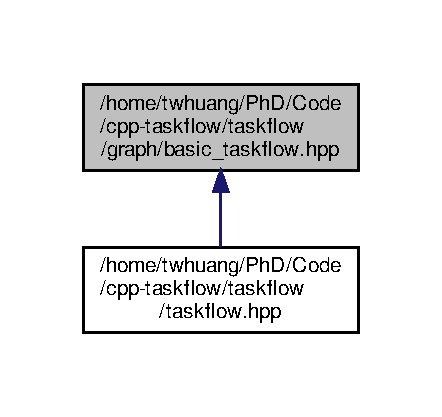
\includegraphics[width=212pt]{basic__taskflow_8hpp__dep__incl}
\end{center}
\end{figure}
\subsection*{Classes}
\begin{DoxyCompactItemize}
\item 
class \hyperlink{classtf_1_1BasicTaskflow}{tf\+::\+Basic\+Taskflow$<$ E $>$}
\end{DoxyCompactItemize}
\subsection*{Namespaces}
\begin{DoxyCompactItemize}
\item 
 \hyperlink{namespacetf}{tf}
\end{DoxyCompactItemize}

\hypertarget{flow__builder_8hpp}{}\section{/home/twhuang/\+Ph\+D/\+Code/cpp-\/taskflow/taskflow/graph/flow\+\_\+builder.hpp File Reference}
\label{flow__builder_8hpp}\index{/home/twhuang/\+Ph\+D/\+Code/cpp-\/taskflow/taskflow/graph/flow\+\_\+builder.\+hpp@{/home/twhuang/\+Ph\+D/\+Code/cpp-\/taskflow/taskflow/graph/flow\+\_\+builder.\+hpp}}
{\ttfamily \#include \char`\"{}graph.\+hpp\char`\"{}}\newline
Include dependency graph for flow\+\_\+builder.\+hpp\+:\nopagebreak
\begin{figure}[H]
\begin{center}
\leavevmode
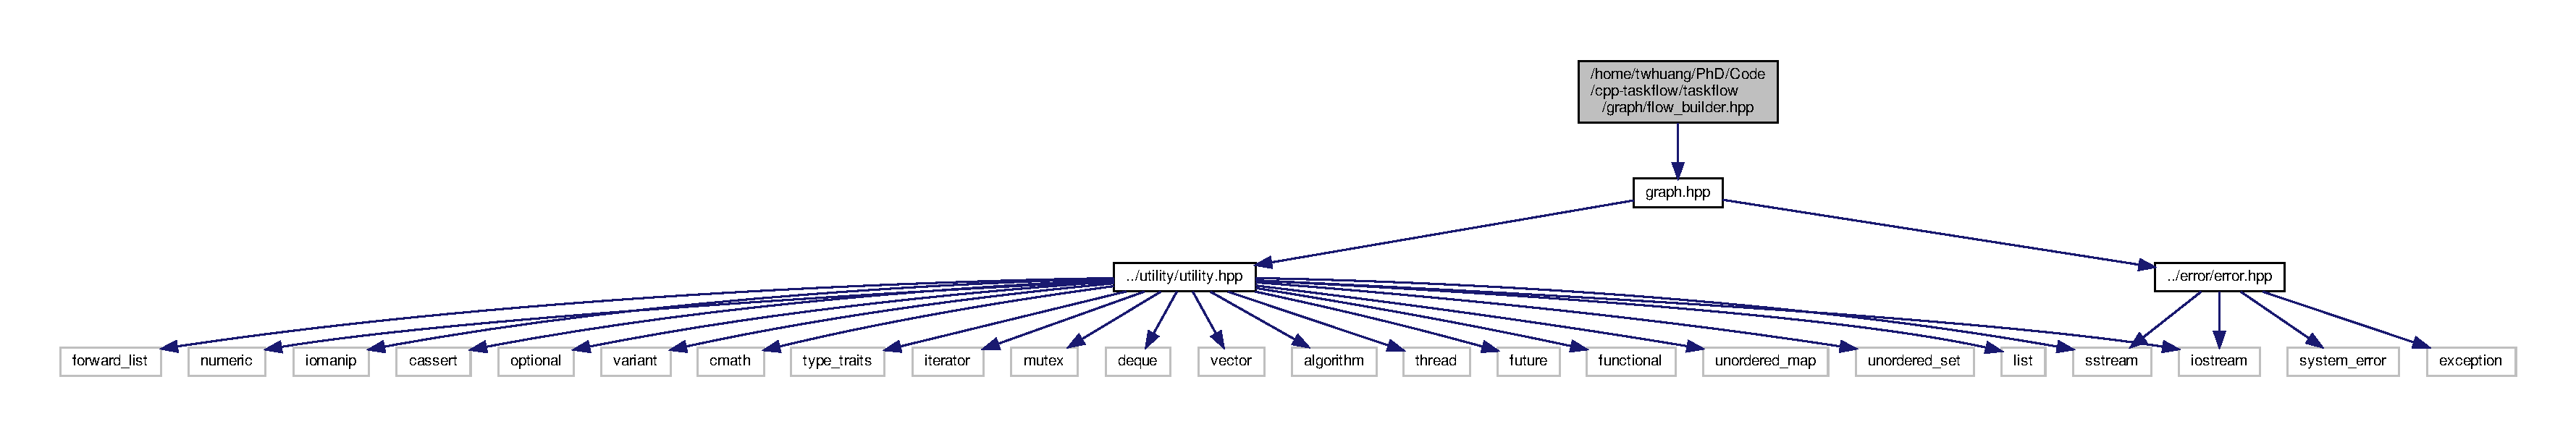
\includegraphics[width=350pt]{flow__builder_8hpp__incl}
\end{center}
\end{figure}
This graph shows which files directly or indirectly include this file\+:\nopagebreak
\begin{figure}[H]
\begin{center}
\leavevmode
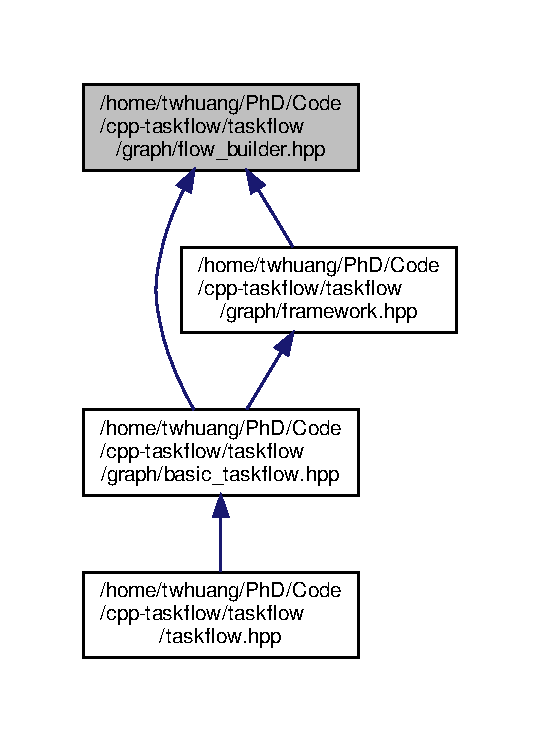
\includegraphics[width=259pt]{flow__builder_8hpp__dep__incl}
\end{center}
\end{figure}
\subsection*{Classes}
\begin{DoxyCompactItemize}
\item 
class \hyperlink{classtf_1_1FlowBuilder}{tf\+::\+Flow\+Builder}
\item 
class \hyperlink{classtf_1_1SubflowBuilder}{tf\+::\+Subflow\+Builder}
\end{DoxyCompactItemize}
\subsection*{Namespaces}
\begin{DoxyCompactItemize}
\item 
 \hyperlink{namespacetf}{tf}
\end{DoxyCompactItemize}

\hypertarget{framework_8hpp}{}\section{/home/twhuang/\+Ph\+D/\+Code/cpp-\/taskflow/taskflow/graph/framework.hpp File Reference}
\label{framework_8hpp}\index{/home/twhuang/\+Ph\+D/\+Code/cpp-\/taskflow/taskflow/graph/framework.\+hpp@{/home/twhuang/\+Ph\+D/\+Code/cpp-\/taskflow/taskflow/graph/framework.\+hpp}}
{\ttfamily \#include \char`\"{}flow\+\_\+builder.\+hpp\char`\"{}}\newline
Include dependency graph for framework.\+hpp\+:\nopagebreak
\begin{figure}[H]
\begin{center}
\leavevmode
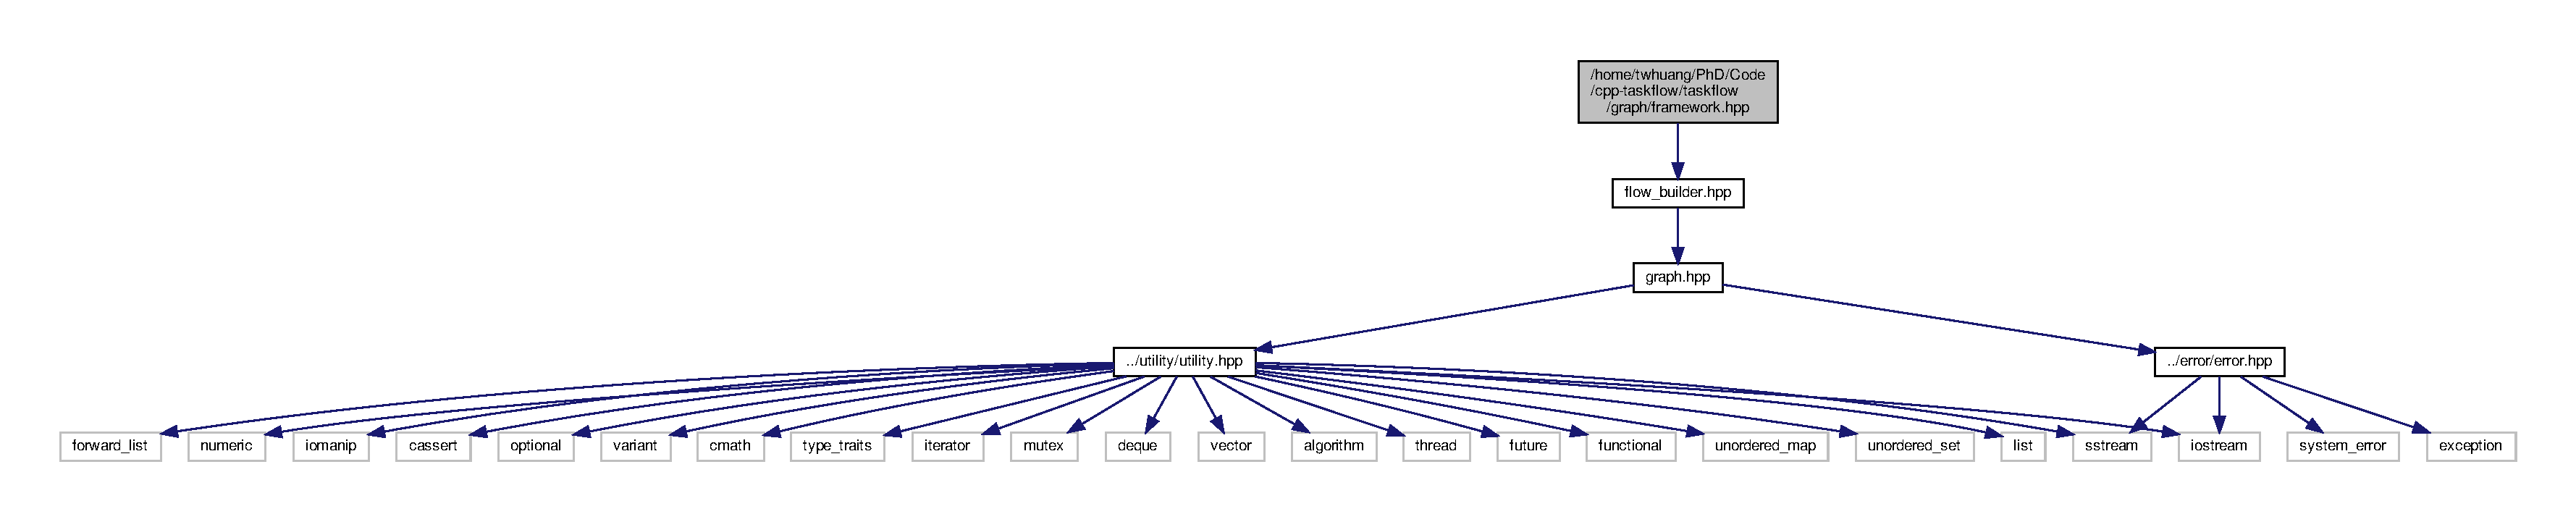
\includegraphics[width=350pt]{framework_8hpp__incl}
\end{center}
\end{figure}
This graph shows which files directly or indirectly include this file\+:\nopagebreak
\begin{figure}[H]
\begin{center}
\leavevmode
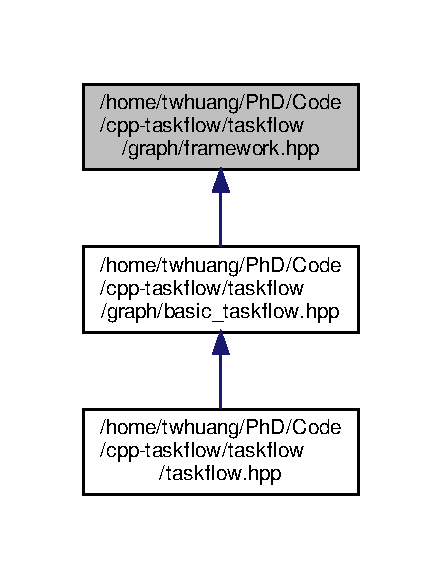
\includegraphics[width=212pt]{framework_8hpp__dep__incl}
\end{center}
\end{figure}
\subsection*{Classes}
\begin{DoxyCompactItemize}
\item 
class \hyperlink{classtf_1_1Framework}{tf\+::\+Framework}
\end{DoxyCompactItemize}
\subsection*{Namespaces}
\begin{DoxyCompactItemize}
\item 
 \hyperlink{namespacetf}{tf}
\end{DoxyCompactItemize}

\hypertarget{graph_8hpp}{}\section{/home/twhuang/\+Ph\+D/\+Code/cpp-\/taskflow/taskflow/graph/graph.hpp File Reference}
\label{graph_8hpp}\index{/home/twhuang/\+Ph\+D/\+Code/cpp-\/taskflow/taskflow/graph/graph.\+hpp@{/home/twhuang/\+Ph\+D/\+Code/cpp-\/taskflow/taskflow/graph/graph.\+hpp}}
{\ttfamily \#include \char`\"{}../error/error.\+hpp\char`\"{}}\newline
{\ttfamily \#include \char`\"{}../utility/utility.\+hpp\char`\"{}}\newline
Include dependency graph for graph.\+hpp\+:\nopagebreak
\begin{figure}[H]
\begin{center}
\leavevmode
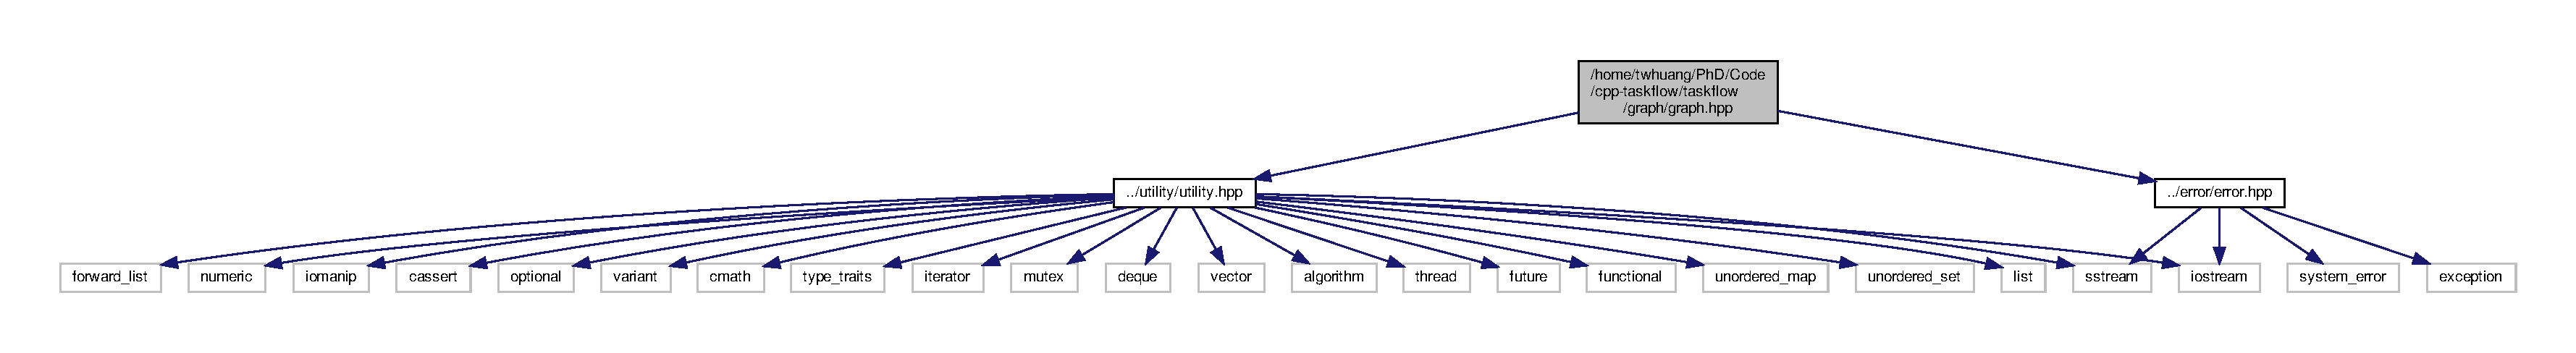
\includegraphics[width=350pt]{graph_8hpp__incl}
\end{center}
\end{figure}
This graph shows which files directly or indirectly include this file\+:\nopagebreak
\begin{figure}[H]
\begin{center}
\leavevmode
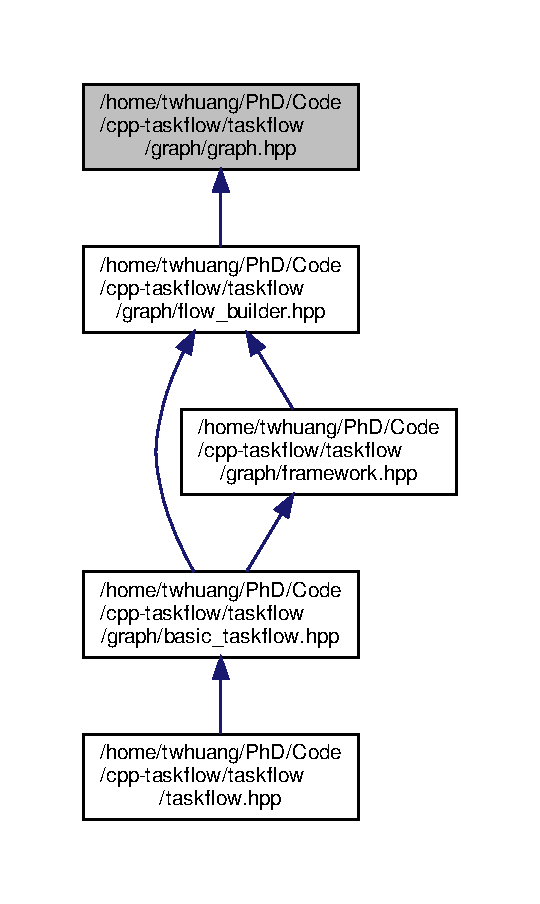
\includegraphics[width=259pt]{graph_8hpp__dep__incl}
\end{center}
\end{figure}
\subsection*{Classes}
\begin{DoxyCompactItemize}
\item 
class \hyperlink{classtf_1_1Node}{tf\+::\+Node}
\item 
class \hyperlink{classtf_1_1Topology}{tf\+::\+Topology}
\item 
class \hyperlink{classtf_1_1Task}{tf\+::\+Task}
\end{DoxyCompactItemize}
\subsection*{Namespaces}
\begin{DoxyCompactItemize}
\item 
 \hyperlink{namespacetf}{tf}
\end{DoxyCompactItemize}
\subsection*{Typedefs}
\begin{DoxyCompactItemize}
\item 
using \hyperlink{namespacetf_a2afa7da139285640eaf8122535136dc9}{tf\+::\+Graph} = std\+::forward\+\_\+list$<$ Node $>$
\end{DoxyCompactItemize}

\hypertarget{taskflow_8hpp}{}\section{/home/twhuang/\+Ph\+D/\+Code/cpp-\/taskflow/taskflow/taskflow.hpp File Reference}
\label{taskflow_8hpp}\index{/home/twhuang/\+Ph\+D/\+Code/cpp-\/taskflow/taskflow/taskflow.\+hpp@{/home/twhuang/\+Ph\+D/\+Code/cpp-\/taskflow/taskflow/taskflow.\+hpp}}
{\ttfamily \#include \char`\"{}graph/basic\+\_\+taskflow.\+hpp\char`\"{}}\newline
Include dependency graph for taskflow.\+hpp\+:\nopagebreak
\begin{figure}[H]
\begin{center}
\leavevmode
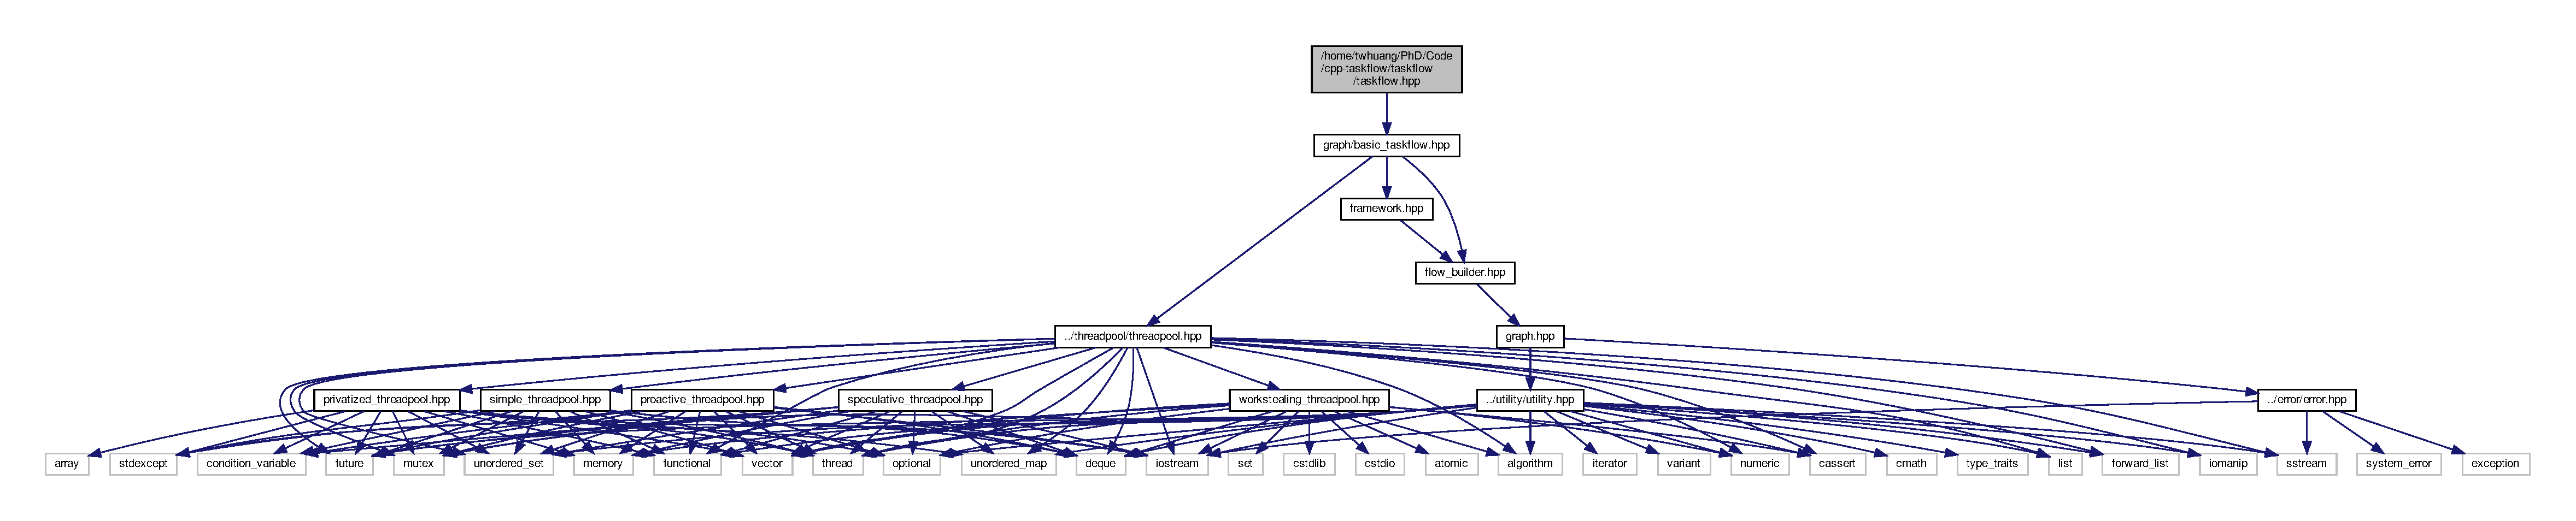
\includegraphics[width=350pt]{taskflow_8hpp__incl}
\end{center}
\end{figure}
\subsection*{Namespaces}
\begin{DoxyCompactItemize}
\item 
 \hyperlink{namespacetf}{tf}
\end{DoxyCompactItemize}
\subsection*{Typedefs}
\begin{DoxyCompactItemize}
\item 
using \hyperlink{namespacetf_aa4b65604639a98fffa65678506be94c9}{tf\+::\+Taskflow} = Basic\+Taskflow$<$ Work\+Stealing\+Threadpool $>$
\end{DoxyCompactItemize}

\hypertarget{privatized__threadpool_8hpp}{}\section{/home/twhuang/\+Ph\+D/\+Code/cpp-\/taskflow/taskflow/threadpool/privatized\+\_\+threadpool.hpp File Reference}
\label{privatized__threadpool_8hpp}\index{/home/twhuang/\+Ph\+D/\+Code/cpp-\/taskflow/taskflow/threadpool/privatized\+\_\+threadpool.\+hpp@{/home/twhuang/\+Ph\+D/\+Code/cpp-\/taskflow/taskflow/threadpool/privatized\+\_\+threadpool.\+hpp}}
{\ttfamily \#include $<$iostream$>$}\newline
{\ttfamily \#include $<$functional$>$}\newline
{\ttfamily \#include $<$vector$>$}\newline
{\ttfamily \#include $<$mutex$>$}\newline
{\ttfamily \#include $<$thread$>$}\newline
{\ttfamily \#include $<$stdexcept$>$}\newline
{\ttfamily \#include $<$condition\+\_\+variable$>$}\newline
{\ttfamily \#include $<$memory$>$}\newline
{\ttfamily \#include $<$future$>$}\newline
{\ttfamily \#include $<$optional$>$}\newline
{\ttfamily \#include $<$unordered\+\_\+set$>$}\newline
{\ttfamily \#include $<$unordered\+\_\+map$>$}\newline
{\ttfamily \#include $<$array$>$}\newline
Include dependency graph for privatized\+\_\+threadpool.\+hpp\+:\nopagebreak
\begin{figure}[H]
\begin{center}
\leavevmode
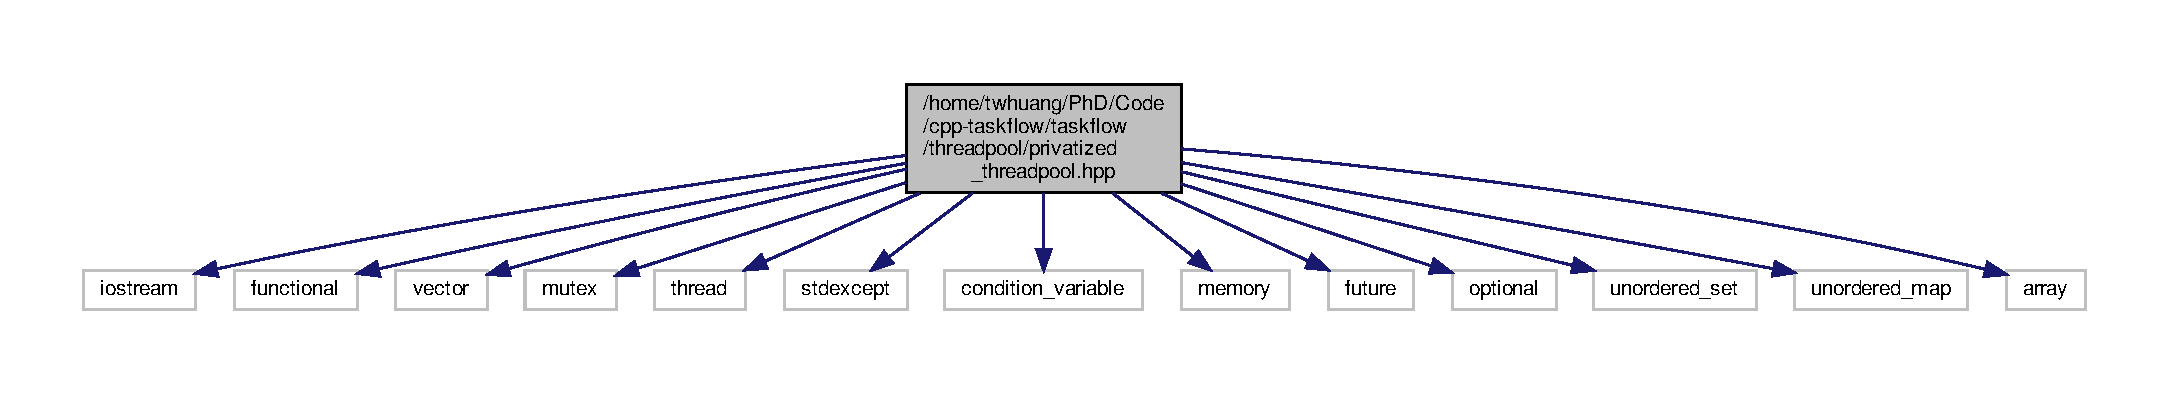
\includegraphics[width=350pt]{privatized__threadpool_8hpp__incl}
\end{center}
\end{figure}
This graph shows which files directly or indirectly include this file\+:\nopagebreak
\begin{figure}[H]
\begin{center}
\leavevmode
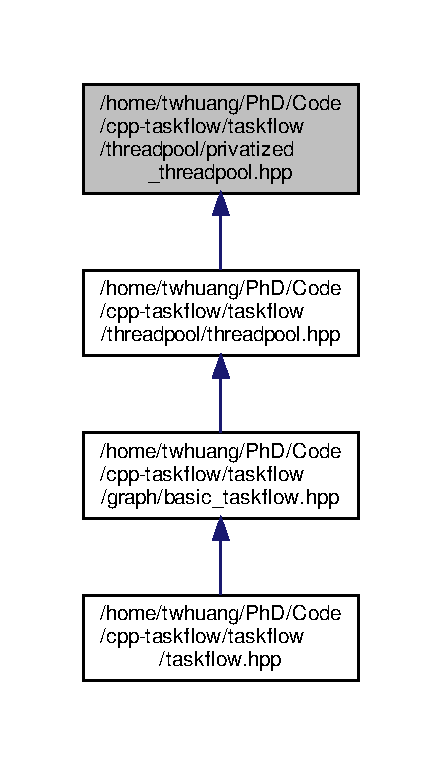
\includegraphics[width=212pt]{privatized__threadpool_8hpp__dep__incl}
\end{center}
\end{figure}
\subsection*{Classes}
\begin{DoxyCompactItemize}
\item 
class \hyperlink{classtf_1_1PrivatizedWorkQueue}{tf\+::\+Privatized\+Work\+Queue$<$ T, C $>$}
\item 
class \hyperlink{classtf_1_1PrivatizedThreadpool}{tf\+::\+Privatized\+Threadpool$<$ Closure $>$}
\end{DoxyCompactItemize}
\subsection*{Namespaces}
\begin{DoxyCompactItemize}
\item 
 \hyperlink{namespacetf}{tf}
\end{DoxyCompactItemize}

\hypertarget{proactive__threadpool_8hpp}{}\section{/home/twhuang/\+Ph\+D/\+Code/cpp-\/taskflow/taskflow/threadpool/proactive\+\_\+threadpool.hpp File Reference}
\label{proactive__threadpool_8hpp}\index{/home/twhuang/\+Ph\+D/\+Code/cpp-\/taskflow/taskflow/threadpool/proactive\+\_\+threadpool.\+hpp@{/home/twhuang/\+Ph\+D/\+Code/cpp-\/taskflow/taskflow/threadpool/proactive\+\_\+threadpool.\+hpp}}
{\ttfamily \#include $<$iostream$>$}\newline
{\ttfamily \#include $<$functional$>$}\newline
{\ttfamily \#include $<$vector$>$}\newline
{\ttfamily \#include $<$mutex$>$}\newline
{\ttfamily \#include $<$deque$>$}\newline
{\ttfamily \#include $<$thread$>$}\newline
{\ttfamily \#include $<$stdexcept$>$}\newline
{\ttfamily \#include $<$condition\+\_\+variable$>$}\newline
{\ttfamily \#include $<$memory$>$}\newline
{\ttfamily \#include $<$future$>$}\newline
{\ttfamily \#include $<$unordered\+\_\+set$>$}\newline
{\ttfamily \#include $<$optional$>$}\newline
Include dependency graph for proactive\+\_\+threadpool.\+hpp\+:\nopagebreak
\begin{figure}[H]
\begin{center}
\leavevmode
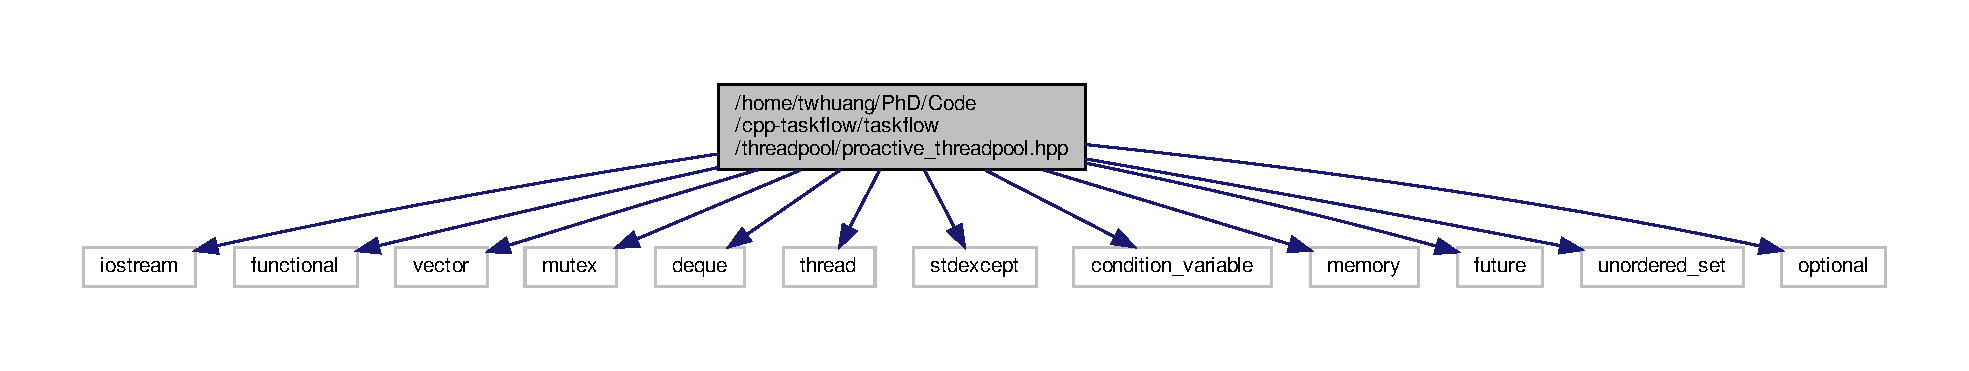
\includegraphics[width=350pt]{proactive__threadpool_8hpp__incl}
\end{center}
\end{figure}
This graph shows which files directly or indirectly include this file\+:\nopagebreak
\begin{figure}[H]
\begin{center}
\leavevmode
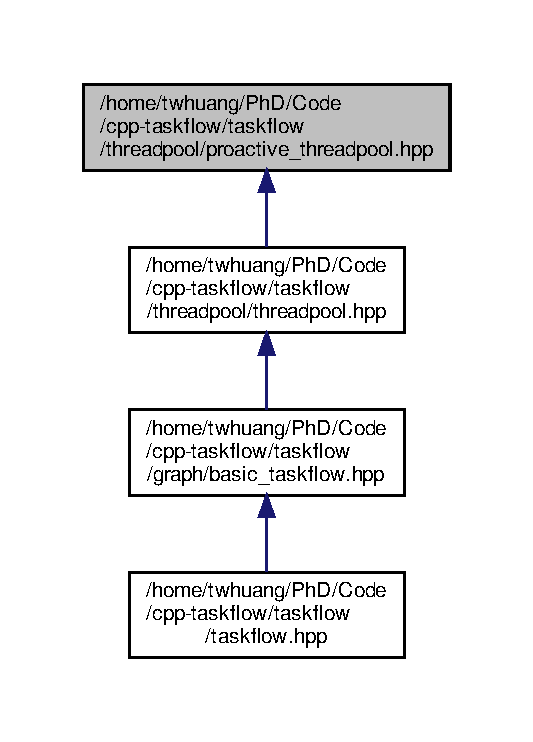
\includegraphics[width=256pt]{proactive__threadpool_8hpp__dep__incl}
\end{center}
\end{figure}
\subsection*{Classes}
\begin{DoxyCompactItemize}
\item 
class \hyperlink{classtf_1_1ProactiveThreadpool}{tf\+::\+Proactive\+Threadpool$<$ Closure $>$}
\end{DoxyCompactItemize}
\subsection*{Namespaces}
\begin{DoxyCompactItemize}
\item 
 \hyperlink{namespacetf}{tf}
\end{DoxyCompactItemize}

\hypertarget{simple__threadpool_8hpp}{}\section{/home/twhuang/\+Ph\+D/\+Code/cpp-\/taskflow/taskflow/threadpool/simple\+\_\+threadpool.hpp File Reference}
\label{simple__threadpool_8hpp}\index{/home/twhuang/\+Ph\+D/\+Code/cpp-\/taskflow/taskflow/threadpool/simple\+\_\+threadpool.\+hpp@{/home/twhuang/\+Ph\+D/\+Code/cpp-\/taskflow/taskflow/threadpool/simple\+\_\+threadpool.\+hpp}}
{\ttfamily \#include $<$iostream$>$}\newline
{\ttfamily \#include $<$functional$>$}\newline
{\ttfamily \#include $<$vector$>$}\newline
{\ttfamily \#include $<$mutex$>$}\newline
{\ttfamily \#include $<$deque$>$}\newline
{\ttfamily \#include $<$thread$>$}\newline
{\ttfamily \#include $<$stdexcept$>$}\newline
{\ttfamily \#include $<$condition\+\_\+variable$>$}\newline
{\ttfamily \#include $<$memory$>$}\newline
{\ttfamily \#include $<$future$>$}\newline
{\ttfamily \#include $<$unordered\+\_\+set$>$}\newline
Include dependency graph for simple\+\_\+threadpool.\+hpp\+:\nopagebreak
\begin{figure}[H]
\begin{center}
\leavevmode
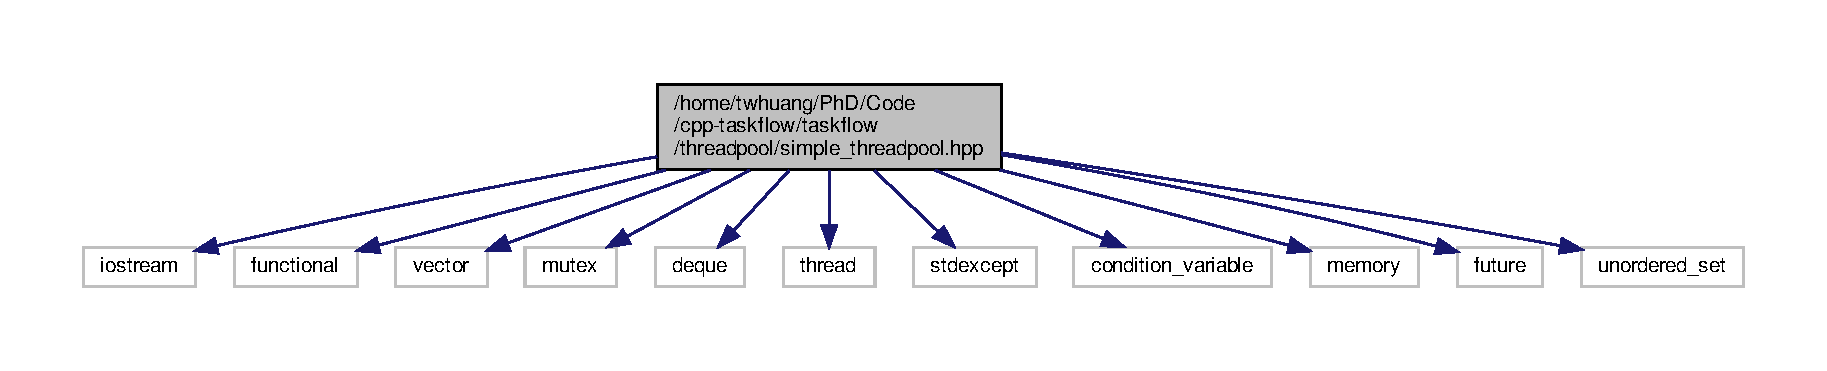
\includegraphics[width=350pt]{simple__threadpool_8hpp__incl}
\end{center}
\end{figure}
This graph shows which files directly or indirectly include this file\+:\nopagebreak
\begin{figure}[H]
\begin{center}
\leavevmode
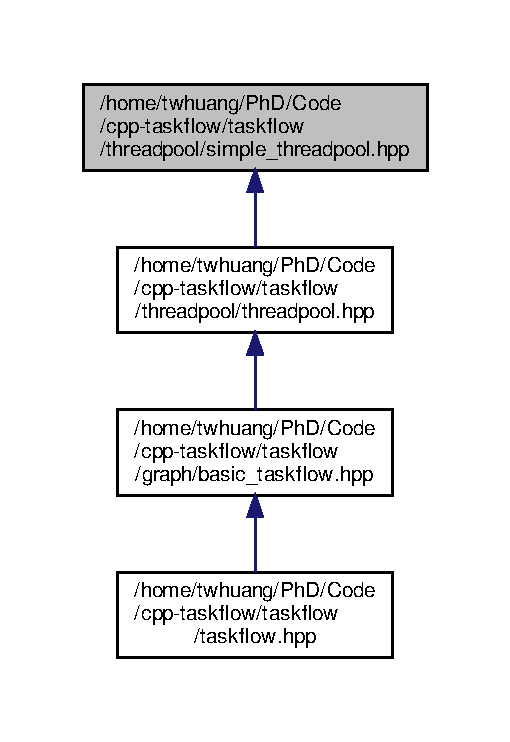
\includegraphics[width=245pt]{simple__threadpool_8hpp__dep__incl}
\end{center}
\end{figure}
\subsection*{Classes}
\begin{DoxyCompactItemize}
\item 
class \hyperlink{classtf_1_1SimpleThreadpool}{tf\+::\+Simple\+Threadpool$<$ Closure $>$}
\end{DoxyCompactItemize}
\subsection*{Namespaces}
\begin{DoxyCompactItemize}
\item 
 \hyperlink{namespacetf}{tf}
\end{DoxyCompactItemize}

\hypertarget{speculative__threadpool_8hpp}{}\section{/home/twhuang/\+Ph\+D/\+Code/cpp-\/taskflow/taskflow/threadpool/speculative\+\_\+threadpool.hpp File Reference}
\label{speculative__threadpool_8hpp}\index{/home/twhuang/\+Ph\+D/\+Code/cpp-\/taskflow/taskflow/threadpool/speculative\+\_\+threadpool.\+hpp@{/home/twhuang/\+Ph\+D/\+Code/cpp-\/taskflow/taskflow/threadpool/speculative\+\_\+threadpool.\+hpp}}
{\ttfamily \#include $<$iostream$>$}\newline
{\ttfamily \#include $<$functional$>$}\newline
{\ttfamily \#include $<$vector$>$}\newline
{\ttfamily \#include $<$mutex$>$}\newline
{\ttfamily \#include $<$deque$>$}\newline
{\ttfamily \#include $<$thread$>$}\newline
{\ttfamily \#include $<$stdexcept$>$}\newline
{\ttfamily \#include $<$condition\+\_\+variable$>$}\newline
{\ttfamily \#include $<$memory$>$}\newline
{\ttfamily \#include $<$future$>$}\newline
{\ttfamily \#include $<$unordered\+\_\+set$>$}\newline
{\ttfamily \#include $<$unordered\+\_\+map$>$}\newline
{\ttfamily \#include $<$optional$>$}\newline
Include dependency graph for speculative\+\_\+threadpool.\+hpp\+:\nopagebreak
\begin{figure}[H]
\begin{center}
\leavevmode
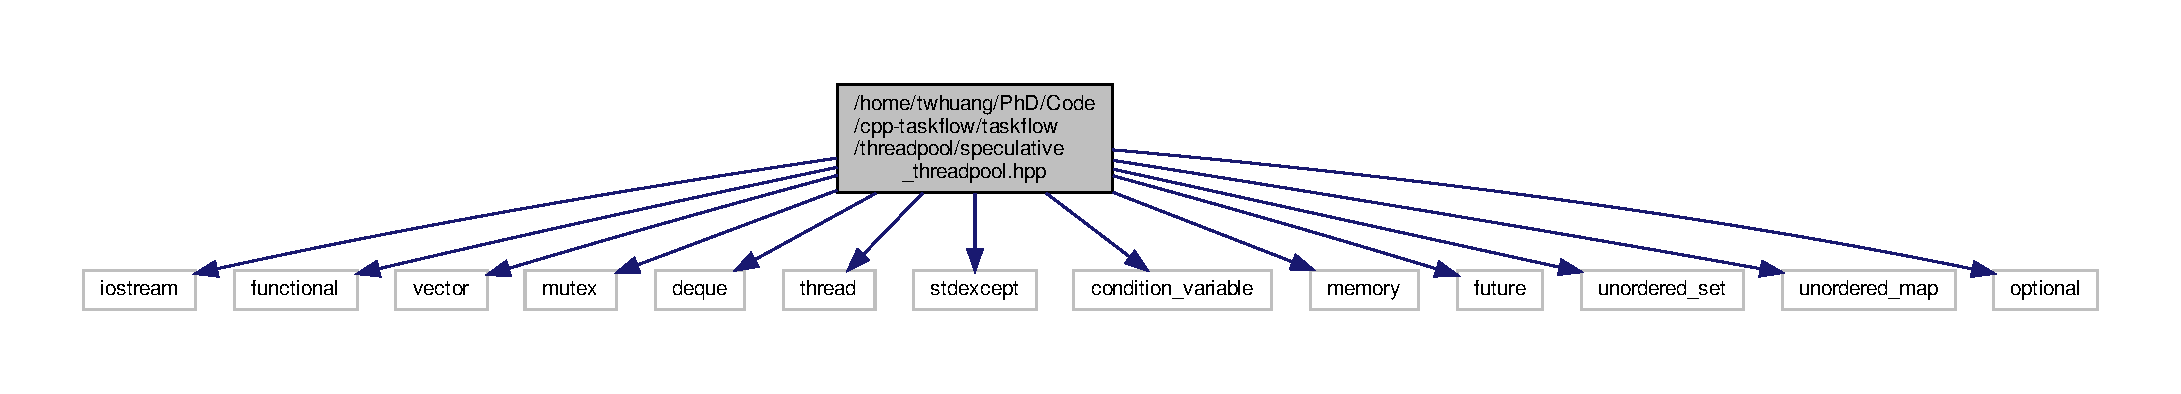
\includegraphics[width=350pt]{speculative__threadpool_8hpp__incl}
\end{center}
\end{figure}
This graph shows which files directly or indirectly include this file\+:\nopagebreak
\begin{figure}[H]
\begin{center}
\leavevmode
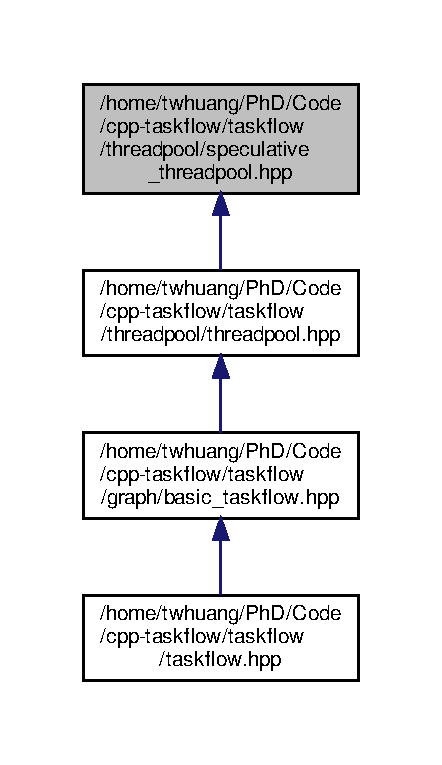
\includegraphics[width=212pt]{speculative__threadpool_8hpp__dep__incl}
\end{center}
\end{figure}
\subsection*{Classes}
\begin{DoxyCompactItemize}
\item 
class \hyperlink{classtf_1_1SpeculativeThreadpool}{tf\+::\+Speculative\+Threadpool$<$ Closure $>$}
\end{DoxyCompactItemize}
\subsection*{Namespaces}
\begin{DoxyCompactItemize}
\item 
 \hyperlink{namespacetf}{tf}
\end{DoxyCompactItemize}

\hypertarget{threadpool_8hpp}{}\section{/home/twhuang/\+Ph\+D/\+Code/cpp-\/taskflow/taskflow/threadpool/threadpool.hpp File Reference}
\label{threadpool_8hpp}\index{/home/twhuang/\+Ph\+D/\+Code/cpp-\/taskflow/taskflow/threadpool/threadpool.\+hpp@{/home/twhuang/\+Ph\+D/\+Code/cpp-\/taskflow/taskflow/threadpool/threadpool.\+hpp}}
{\ttfamily \#include $<$iostream$>$}\newline
{\ttfamily \#include $<$mutex$>$}\newline
{\ttfamily \#include $<$deque$>$}\newline
{\ttfamily \#include $<$vector$>$}\newline
{\ttfamily \#include $<$algorithm$>$}\newline
{\ttfamily \#include $<$thread$>$}\newline
{\ttfamily \#include $<$future$>$}\newline
{\ttfamily \#include $<$functional$>$}\newline
{\ttfamily \#include $<$unordered\+\_\+map$>$}\newline
{\ttfamily \#include $<$unordered\+\_\+set$>$}\newline
{\ttfamily \#include $<$sstream$>$}\newline
{\ttfamily \#include $<$list$>$}\newline
{\ttfamily \#include $<$forward\+\_\+list$>$}\newline
{\ttfamily \#include $<$numeric$>$}\newline
{\ttfamily \#include $<$iomanip$>$}\newline
{\ttfamily \#include $<$cassert$>$}\newline
{\ttfamily \#include \char`\"{}simple\+\_\+threadpool.\+hpp\char`\"{}}\newline
{\ttfamily \#include \char`\"{}proactive\+\_\+threadpool.\+hpp\char`\"{}}\newline
{\ttfamily \#include \char`\"{}speculative\+\_\+threadpool.\+hpp\char`\"{}}\newline
{\ttfamily \#include \char`\"{}privatized\+\_\+threadpool.\+hpp\char`\"{}}\newline
{\ttfamily \#include \char`\"{}workstealing\+\_\+threadpool.\+hpp\char`\"{}}\newline
Include dependency graph for threadpool.\+hpp\+:\nopagebreak
\begin{figure}[H]
\begin{center}
\leavevmode
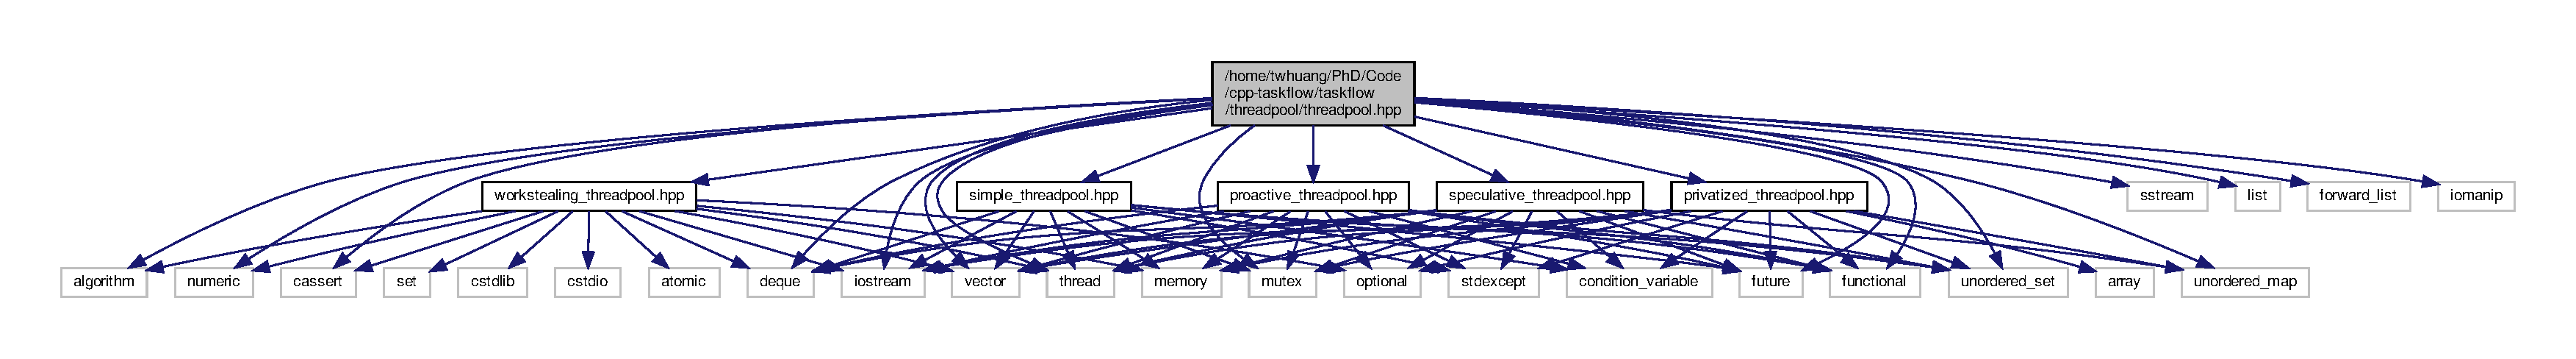
\includegraphics[width=350pt]{threadpool_8hpp__incl}
\end{center}
\end{figure}
This graph shows which files directly or indirectly include this file\+:\nopagebreak
\begin{figure}[H]
\begin{center}
\leavevmode
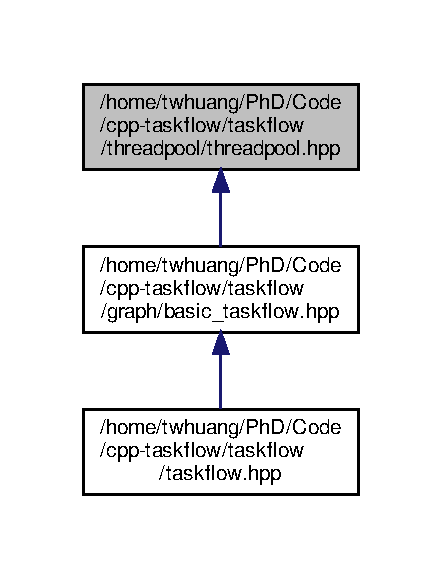
\includegraphics[width=212pt]{threadpool_8hpp__dep__incl}
\end{center}
\end{figure}
\subsection*{Namespaces}
\begin{DoxyCompactItemize}
\item 
 \hyperlink{namespacetf}{tf}
\end{DoxyCompactItemize}

\hypertarget{threadpool__cxx14_8hpp}{}\section{/home/twhuang/\+Ph\+D/\+Code/cpp-\/taskflow/taskflow/threadpool/threadpool\+\_\+cxx14.hpp File Reference}
\label{threadpool__cxx14_8hpp}\index{/home/twhuang/\+Ph\+D/\+Code/cpp-\/taskflow/taskflow/threadpool/threadpool\+\_\+cxx14.\+hpp@{/home/twhuang/\+Ph\+D/\+Code/cpp-\/taskflow/taskflow/threadpool/threadpool\+\_\+cxx14.\+hpp}}
{\ttfamily \#include $<$deque$>$}\newline
{\ttfamily \#include $<$vector$>$}\newline
{\ttfamily \#include $<$thread$>$}\newline
{\ttfamily \#include $<$future$>$}\newline
{\ttfamily \#include $<$unordered\+\_\+set$>$}\newline
{\ttfamily \#include $<$type\+\_\+traits$>$}\newline
{\ttfamily \#include $<$utility$>$}\newline
Include dependency graph for threadpool\+\_\+cxx14.\+hpp\+:\nopagebreak
\begin{figure}[H]
\begin{center}
\leavevmode
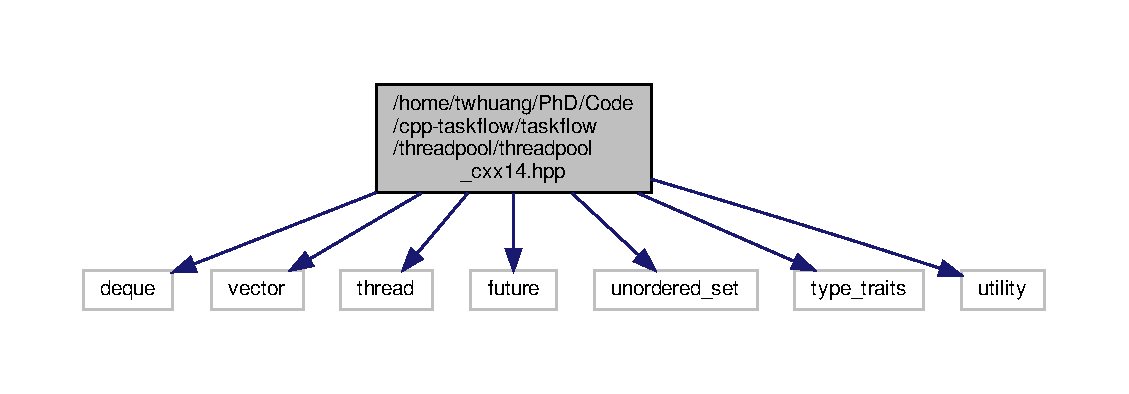
\includegraphics[width=350pt]{threadpool__cxx14_8hpp__incl}
\end{center}
\end{figure}
\subsection*{Classes}
\begin{DoxyCompactItemize}
\item 
struct \hyperlink{structstd_1_1detail_1_1is__reference__wrapper}{std\+::detail\+::is\+\_\+reference\+\_\+wrapper$<$ T $>$}
\item 
struct \hyperlink{structstd_1_1detail_1_1is__reference__wrapper_3_01std_1_1reference__wrapper_3_01U_01_4_01_4}{std\+::detail\+::is\+\_\+reference\+\_\+wrapper$<$ std\+::reference\+\_\+wrapper$<$ U $>$ $>$}
\item 
struct \hyperlink{structstd_1_1detail_1_1invoke__impl}{std\+::detail\+::invoke\+\_\+impl$<$ T $>$}
\item 
struct \hyperlink{structstd_1_1detail_1_1invoke__impl_3_01MT_01B_1_1_5_01_4}{std\+::detail\+::invoke\+\_\+impl$<$ M\+T B\+::$\ast$ $>$}
\item 
struct \hyperlink{structstd_1_1detail_1_1invoke__result}{std\+::detail\+::invoke\+\_\+result$<$ Always\+Void, typename,... $>$}
\item 
struct \hyperlink{structstd_1_1detail_1_1invoke__result_3_01decltype_07void_07detail_1_1INVOKE_07std_1_1declval_3_86a9900dcd4a84f000244f479e0f71a8}{std\+::detail\+::invoke\+\_\+result$<$ decltype(void(detail\+::\+I\+N\+V\+O\+K\+E(std\+::declval$<$ F $>$(), std\+::declval$<$ Args $>$()...))), F, Args... $>$}
\item 
struct \hyperlink{structstd_1_1invoke__result}{std\+::invoke\+\_\+result$<$ F, Arg\+Types $>$}
\item 
struct \hyperlink{structtf_1_1MoC}{tf\+::\+Mo\+C$<$ T $>$}
\item 
class \hyperlink{classtf_1_1Threadpool}{tf\+::\+Threadpool}
\end{DoxyCompactItemize}
\subsection*{Namespaces}
\begin{DoxyCompactItemize}
\item 
 \hyperlink{namespacestd}{std}
\item 
 \hyperlink{namespacestd_1_1detail}{std\+::detail}
\item 
 \hyperlink{namespacetf}{tf}
\end{DoxyCompactItemize}
\subsection*{Typedefs}
\begin{DoxyCompactItemize}
\item 
{\footnotesize template$<$class F , class... Arg\+Types$>$ }\\using \hyperlink{namespacestd_a492e7f3c5595a8b7a7c6e0c9294f5c81}{std\+::invoke\+\_\+result\+\_\+t} = typename invoke\+\_\+result$<$ F, Arg\+Types... $>$\+::type
\end{DoxyCompactItemize}
\subsection*{Functions}
\begin{DoxyCompactItemize}
\item 
{\footnotesize template$<$class F , class... Args, class Fd  = typename std\+::decay$<$\+F$>$\+::type$>$ }\\auto \hyperlink{namespacestd_1_1detail_ac5263dda7d727dde5281b6b1da8ebb79}{std\+::detail\+::\+I\+N\+V\+O\+KE} (F \&\&f, Args \&\&... args) -\/$>$ decltype(invoke\+\_\+impl$<$ Fd $>$\+::call(std\+::forward$<$ F $>$(f), std\+::forward$<$ Args $>$(args)...))
\end{DoxyCompactItemize}

\hypertarget{workstealing__threadpool_8hpp}{}\section{/home/twhuang/\+Ph\+D/\+Code/cpp-\/taskflow/taskflow/threadpool/workstealing\+\_\+threadpool.hpp File Reference}
\label{workstealing__threadpool_8hpp}\index{/home/twhuang/\+Ph\+D/\+Code/cpp-\/taskflow/taskflow/threadpool/workstealing\+\_\+threadpool.\+hpp@{/home/twhuang/\+Ph\+D/\+Code/cpp-\/taskflow/taskflow/threadpool/workstealing\+\_\+threadpool.\+hpp}}
{\ttfamily \#include $<$iostream$>$}\newline
{\ttfamily \#include $<$vector$>$}\newline
{\ttfamily \#include $<$cstdlib$>$}\newline
{\ttfamily \#include $<$cstdio$>$}\newline
{\ttfamily \#include $<$atomic$>$}\newline
{\ttfamily \#include $<$memory$>$}\newline
{\ttfamily \#include $<$cassert$>$}\newline
{\ttfamily \#include $<$deque$>$}\newline
{\ttfamily \#include $<$optional$>$}\newline
{\ttfamily \#include $<$thread$>$}\newline
{\ttfamily \#include $<$algorithm$>$}\newline
{\ttfamily \#include $<$set$>$}\newline
{\ttfamily \#include $<$numeric$>$}\newline
Include dependency graph for workstealing\+\_\+threadpool.\+hpp\+:\nopagebreak
\begin{figure}[H]
\begin{center}
\leavevmode
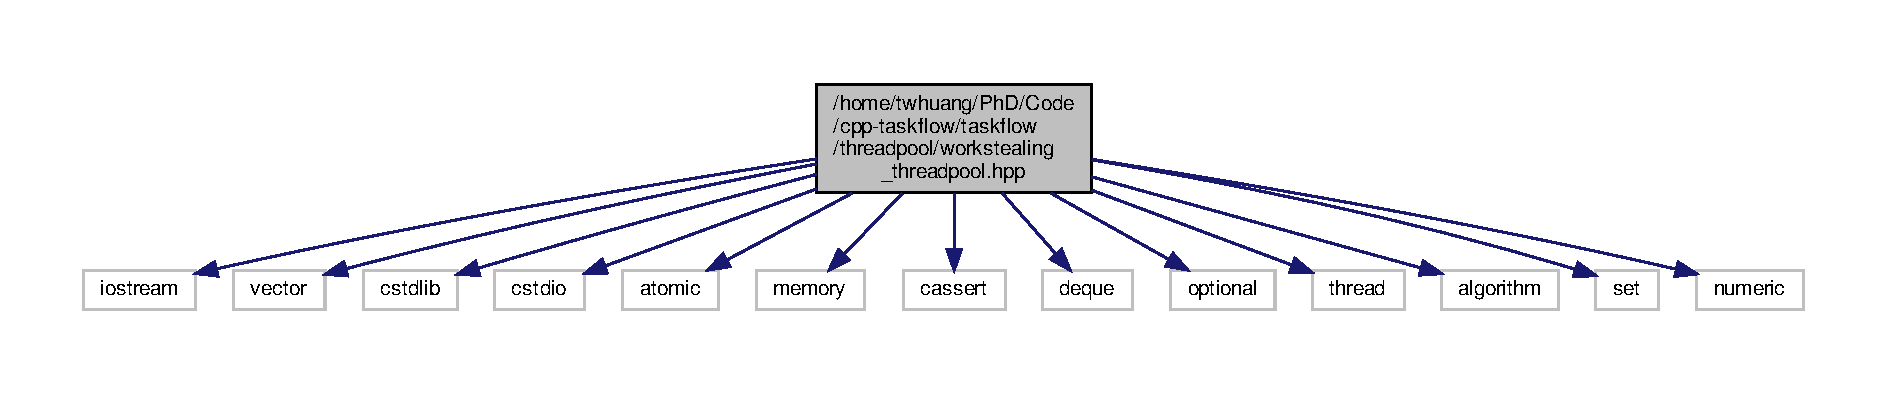
\includegraphics[width=350pt]{workstealing__threadpool_8hpp__incl}
\end{center}
\end{figure}
This graph shows which files directly or indirectly include this file\+:\nopagebreak
\begin{figure}[H]
\begin{center}
\leavevmode
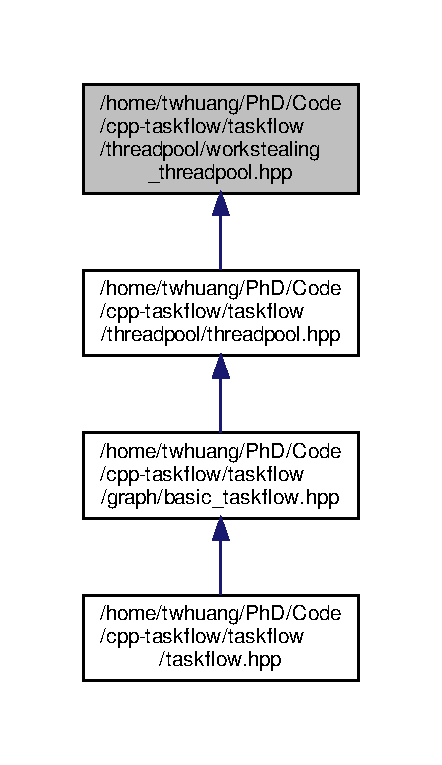
\includegraphics[width=212pt]{workstealing__threadpool_8hpp__dep__incl}
\end{center}
\end{figure}
\subsection*{Classes}
\begin{DoxyCompactItemize}
\item 
class \hyperlink{classtf_1_1WorkStealingQueue}{tf\+::\+Work\+Stealing\+Queue$<$ T $>$}
\item 
class \hyperlink{classtf_1_1WorkStealingThreadpool}{tf\+::\+Work\+Stealing\+Threadpool$<$ Closure $>$}
\end{DoxyCompactItemize}
\subsection*{Namespaces}
\begin{DoxyCompactItemize}
\item 
 \hyperlink{namespacetf}{tf}
\end{DoxyCompactItemize}

\hypertarget{utility_8hpp}{}\section{/home/twhuang/\+Ph\+D/\+Code/cpp-\/taskflow/taskflow/utility/utility.hpp File Reference}
\label{utility_8hpp}\index{/home/twhuang/\+Ph\+D/\+Code/cpp-\/taskflow/taskflow/utility/utility.\+hpp@{/home/twhuang/\+Ph\+D/\+Code/cpp-\/taskflow/taskflow/utility/utility.\+hpp}}
{\ttfamily \#include $<$type\+\_\+traits$>$}\newline
{\ttfamily \#include $<$iterator$>$}\newline
{\ttfamily \#include $<$iostream$>$}\newline
{\ttfamily \#include $<$mutex$>$}\newline
{\ttfamily \#include $<$deque$>$}\newline
{\ttfamily \#include $<$vector$>$}\newline
{\ttfamily \#include $<$algorithm$>$}\newline
{\ttfamily \#include $<$thread$>$}\newline
{\ttfamily \#include $<$future$>$}\newline
{\ttfamily \#include $<$functional$>$}\newline
{\ttfamily \#include $<$unordered\+\_\+map$>$}\newline
{\ttfamily \#include $<$unordered\+\_\+set$>$}\newline
{\ttfamily \#include $<$sstream$>$}\newline
{\ttfamily \#include $<$list$>$}\newline
{\ttfamily \#include $<$forward\+\_\+list$>$}\newline
{\ttfamily \#include $<$numeric$>$}\newline
{\ttfamily \#include $<$iomanip$>$}\newline
{\ttfamily \#include $<$cassert$>$}\newline
{\ttfamily \#include $<$optional$>$}\newline
{\ttfamily \#include $<$variant$>$}\newline
{\ttfamily \#include $<$cmath$>$}\newline
Include dependency graph for utility.\+hpp\+:\nopagebreak
\begin{figure}[H]
\begin{center}
\leavevmode
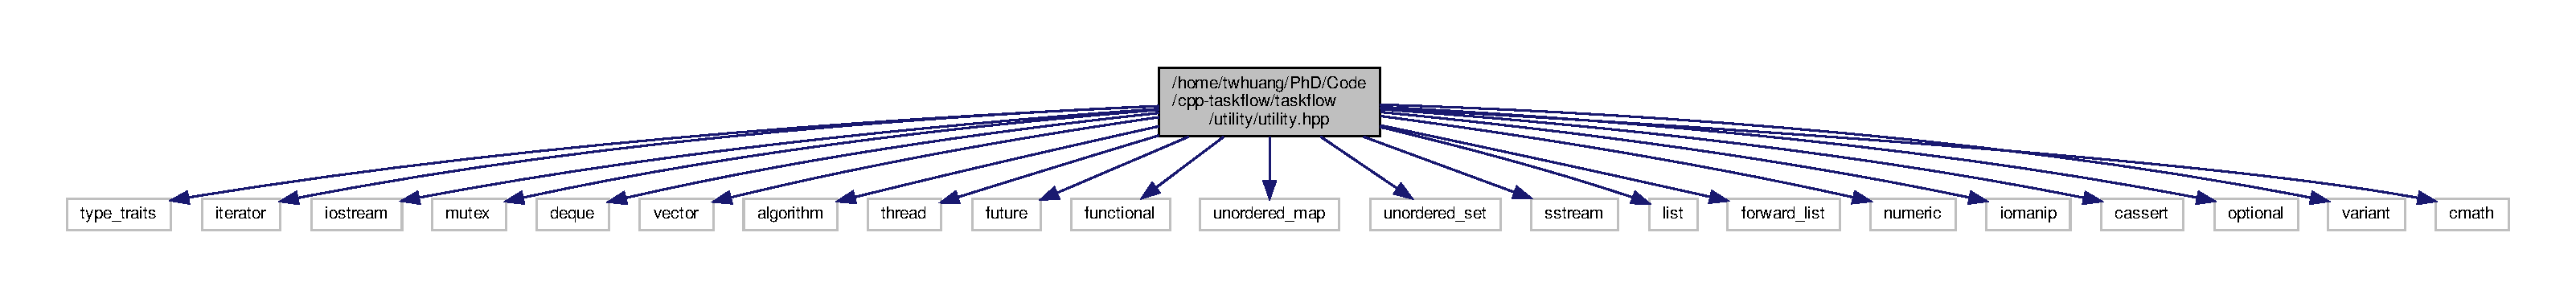
\includegraphics[width=350pt]{utility_8hpp__incl}
\end{center}
\end{figure}
This graph shows which files directly or indirectly include this file\+:\nopagebreak
\begin{figure}[H]
\begin{center}
\leavevmode
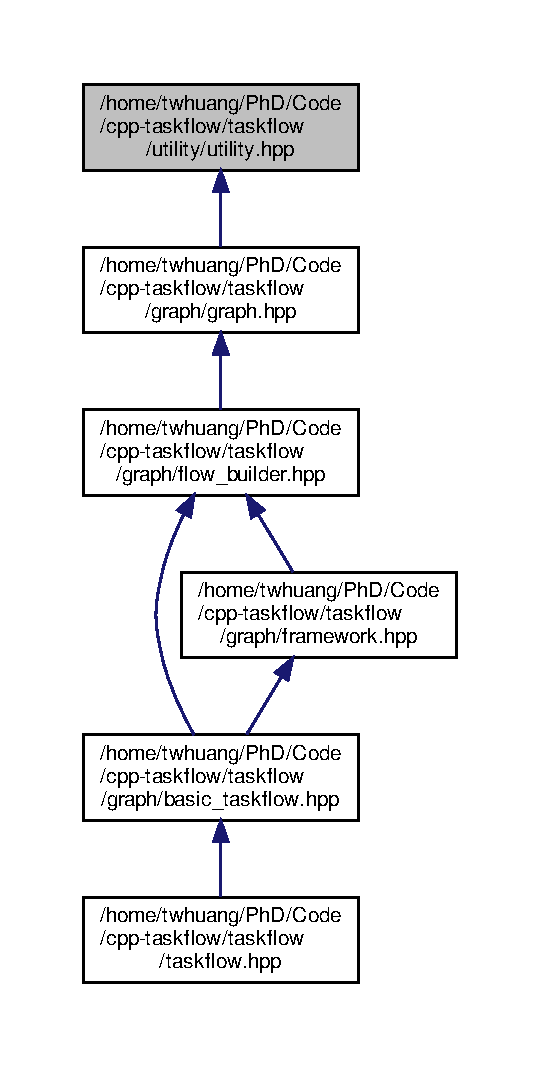
\includegraphics[width=259pt]{utility_8hpp__dep__incl}
\end{center}
\end{figure}
\subsection*{Classes}
\begin{DoxyCompactItemize}
\item 
struct \hyperlink{structtf_1_1dependent__false}{tf\+::dependent\+\_\+false$<$ T $>$}
\item 
struct \hyperlink{structtf_1_1is__iterator}{tf\+::is\+\_\+iterator$<$ T, typename $>$}
\item 
struct \hyperlink{structtf_1_1is__iterator_3_01T_00_01std_1_1enable__if__t_3_9std_1_1is__same__v_3_01typename_01st0a3680c192bddd4961327b11d4422a82}{tf\+::is\+\_\+same\+\_\+v$<$ typename std\+::iterator\+\_\+traits$<$ T $>$\+::value\+\_\+type, void $>$ $>$$>$}
\item 
struct \hyperlink{structtf_1_1is__iterable}{tf\+::is\+\_\+iterable$<$ T, typename $>$}
\item 
struct \hyperlink{structtf_1_1is__iterable_3_01T_00_01std_1_1void__t_3_01decltype_07std_1_1declval_3_01T_01_4_07_0275ba78d7ba399cf74de163921d814a0}{tf\+::is\+\_\+iterable$<$ T, std\+::void\+\_\+t$<$ decltype(std\+::declval$<$ T $>$().\+begin()), decltype(std\+::declval$<$ T $>$().\+end())$>$ $>$}
\item 
struct \hyperlink{structtf_1_1MoC}{tf\+::\+Mo\+C$<$ T $>$}
\end{DoxyCompactItemize}
\subsection*{Namespaces}
\begin{DoxyCompactItemize}
\item 
 \hyperlink{namespacetf}{tf}
\end{DoxyCompactItemize}
\subsection*{Macros}
\begin{DoxyCompactItemize}
\item 
\#define \hyperlink{utility_8hpp_a3ce2e076b272787ae6d66cc806bbbe79}{define\+\_\+has\+\_\+member}(member\+\_\+name)
\item 
\#define \hyperlink{utility_8hpp_aa0342ec76cf9ac1ddcee3e1de7e8d497}{has\+\_\+member}(class\+\_\+,  member\+\_\+name)~has\+\_\+member\+\_\+\#\#member\+\_\+name$<$class\+\_\+$>$\+::value
\end{DoxyCompactItemize}
\subsection*{Variables}
\begin{DoxyCompactItemize}
\item 
{\footnotesize template$<$typename... T$>$ }\\constexpr auto \hyperlink{namespacetf_ac47db20fe8976148fb7523a31a1039ce}{tf\+::dependent\+\_\+false\+\_\+v} = dependent\+\_\+false$<$T...$>$\+::value
\item 
{\footnotesize template$<$typename T $>$ }\\constexpr bool \hyperlink{namespacetf_a7492bd7f91002715d38e477e86ec38c9}{tf\+::is\+\_\+iterator\+\_\+v} = is\+\_\+iterator$<$T$>$\+::value
\item 
{\footnotesize template$<$typename T $>$ }\\constexpr bool \hyperlink{namespacetf_a19ce57208fa48a058ae54864d4b343f3}{tf\+::is\+\_\+iterable\+\_\+v} = is\+\_\+iterable$<$T$>$\+::value
\end{DoxyCompactItemize}


\subsection{Macro Definition Documentation}
\mbox{\Hypertarget{utility_8hpp_a3ce2e076b272787ae6d66cc806bbbe79}\label{utility_8hpp_a3ce2e076b272787ae6d66cc806bbbe79}} 
\index{utility.\+hpp@{utility.\+hpp}!define\+\_\+has\+\_\+member@{define\+\_\+has\+\_\+member}}
\index{define\+\_\+has\+\_\+member@{define\+\_\+has\+\_\+member}!utility.\+hpp@{utility.\+hpp}}
\subsubsection{\texorpdfstring{define\+\_\+has\+\_\+member}{define\_has\_member}}
{\footnotesize\ttfamily \#define define\+\_\+has\+\_\+member(\begin{DoxyParamCaption}\item[{}]{member\+\_\+name }\end{DoxyParamCaption})}

{\bfseries Value\+:}
\begin{DoxyCode}
\textcolor{keyword}{template} <\textcolor{keyword}{typename} T>                                                      \(\backslash\)
class has\_member\_##member\_name                                             \(\backslash\)
\{                                                                          \(\backslash\)
  typedef \textcolor{keywordtype}{char} yes\_type;                                                   \(\backslash\)
  typedef \textcolor{keywordtype}{long} no\_type;                                                    \(\backslash\)
  template <typename U> \textcolor{keyword}{static} yes\_type test(decltype(&U::member\_name));   \(\backslash\)
  template <typename U> \textcolor{keyword}{static} no\_type  test(...);                         \(\backslash\)
  public:                                                                  \(\backslash\)
    static constexpr \textcolor{keywordtype}{bool} value = \textcolor{keyword}{sizeof}(test<T>(0)) == \textcolor{keyword}{sizeof}(yes\_type);  \(\backslash\)
\}
\end{DoxyCode}
\mbox{\Hypertarget{utility_8hpp_aa0342ec76cf9ac1ddcee3e1de7e8d497}\label{utility_8hpp_aa0342ec76cf9ac1ddcee3e1de7e8d497}} 
\index{utility.\+hpp@{utility.\+hpp}!has\+\_\+member@{has\+\_\+member}}
\index{has\+\_\+member@{has\+\_\+member}!utility.\+hpp@{utility.\+hpp}}
\subsubsection{\texorpdfstring{has\+\_\+member}{has\_member}}
{\footnotesize\ttfamily \#define has\+\_\+member(\begin{DoxyParamCaption}\item[{}]{class\+\_\+,  }\item[{}]{member\+\_\+name }\end{DoxyParamCaption})~has\+\_\+member\+\_\+\#\#member\+\_\+name$<$class\+\_\+$>$\+::value}


%--- End generated contents ---

% Index
\backmatter
\newpage
\phantomsection
\clearemptydoublepage
\addcontentsline{toc}{chapter}{Index}
\printindex

\end{document}
